\chapter{Auswertung}
\label{text:auswertung}
Die Auswertung von Aufnahmen wird durch ihre Größe erschwert. In einer Aufnahme-Session wird es ca. \numrange{75000}{100000} Aufnahmen gemacht, die insgesamt ca. 180GB groß sind. Jede Aufnahme muss einzeln und kann von anderen Aufnahmen unabhängig ausgewertet werden. So ist der Auswertungsvorgang leicht parallelisierbar. Benutzt wird die „high-level“ API Bibliothek \textit{dask-image} \cite{dask-library}, die parallelisierte und optimierte Ausführung der eingegebenen Funktionen ohne großen technischen Aufwand zulässt.

\noindent
Das gemitteltes Dunkelbild von \num{10000} aufgenommenen Dunkelbildern wird ermittelt und als einzelnes Bild gespeichert. In dem Bild soll das statistische Rauschen durch die Mittlung über große Aufnahmenzahl eliminiert. So bleibt lediglich der konstante Offset von jedem Pixel in dem Bild, der erwartet groß sein soll. Das gemittelte Bild wird von jeder Aufnahme vor der weiteren Auswertung subtrahiert.

\noindent
Die resultierende Differenz, die in der Abb. \ref{fig:capture_ped_diff}c) abgebildet ist, ist, wie erwartet, extrem klein gegenüber das Rohbild und das gemittelte Dunkelbild, die in der Abb. \ref{fig:capture_ped_diff}a) bzw. \ref{fig:capture_ped_diff}b) zu sehen sind. 
\begin{figure}[H]
    \centering
    %% Creator: Matplotlib, PGF backend
%%
%% To include the figure in your LaTeX document, write
%%   \input{<filename>.pgf}
%%
%% Make sure the required packages are loaded in your preamble
%%   \usepackage{pgf}
%%
%% Also ensure that all the required font packages are loaded; for instance,
%% the lmodern package is sometimes necessary when using math font.
%%   \usepackage{lmodern}
%%
%% Figures using additional raster images can only be included by \input if
%% they are in the same directory as the main LaTeX file. For loading figures
%% from other directories you can use the `import` package
%%   \usepackage{import}
%%
%% and then include the figures with
%%   \import{<path to file>}{<filename>.pgf}
%%
%% Matplotlib used the following preamble
%%   \usepackage{amsmath} \usepackage[utf8]{inputenc} \usepackage[T1]{fontenc} \usepackage[output-decimal-marker={,},print-unity-mantissa=false]{siunitx} \sisetup{per-mode=fraction, separate-uncertainty = true, locale = DE} \usepackage[acronym, toc, section=section, nonumberlist, nopostdot]{glossaries-extra}
%%
\begingroup%
\makeatletter%
\begin{pgfpicture}%
\pgfpathrectangle{\pgfpointorigin}{\pgfqpoint{5.886400in}{2.465419in}}%
\pgfusepath{use as bounding box, clip}%
\begin{pgfscope}%
\pgfsetbuttcap%
\pgfsetmiterjoin%
\pgfsetlinewidth{0.000000pt}%
\definecolor{currentstroke}{rgb}{1.000000,1.000000,1.000000}%
\pgfsetstrokecolor{currentstroke}%
\pgfsetstrokeopacity{0.000000}%
\pgfsetdash{}{0pt}%
\pgfpathmoveto{\pgfqpoint{0.000000in}{0.000000in}}%
\pgfpathlineto{\pgfqpoint{5.886400in}{0.000000in}}%
\pgfpathlineto{\pgfqpoint{5.886400in}{2.465419in}}%
\pgfpathlineto{\pgfqpoint{0.000000in}{2.465419in}}%
\pgfpathlineto{\pgfqpoint{0.000000in}{0.000000in}}%
\pgfpathclose%
\pgfusepath{}%
\end{pgfscope}%
\begin{pgfscope}%
\pgfsetbuttcap%
\pgfsetmiterjoin%
\pgfsetlinewidth{0.000000pt}%
\definecolor{currentstroke}{rgb}{1.000000,1.000000,1.000000}%
\pgfsetstrokecolor{currentstroke}%
\pgfsetstrokeopacity{0.000000}%
\pgfsetdash{}{0pt}%
\pgfpathmoveto{\pgfqpoint{-0.377600in}{-1.556873in}}%
\pgfpathlineto{\pgfqpoint{3.942400in}{-1.556873in}}%
\pgfpathlineto{\pgfqpoint{3.942400in}{3.943127in}}%
\pgfpathlineto{\pgfqpoint{-0.377600in}{3.943127in}}%
\pgfpathlineto{\pgfqpoint{-0.377600in}{-1.556873in}}%
\pgfpathclose%
\pgfusepath{}%
\end{pgfscope}%
\begin{pgfscope}%
\pgfsetbuttcap%
\pgfsetmiterjoin%
\definecolor{currentfill}{rgb}{1.000000,1.000000,1.000000}%
\pgfsetfillcolor{currentfill}%
\pgfsetlinewidth{0.000000pt}%
\definecolor{currentstroke}{rgb}{0.000000,0.000000,0.000000}%
\pgfsetstrokecolor{currentstroke}%
\pgfsetstrokeopacity{0.000000}%
\pgfsetdash{}{0pt}%
\pgfpathmoveto{\pgfqpoint{0.162400in}{0.544877in}}%
\pgfpathlineto{\pgfqpoint{1.786400in}{0.544877in}}%
\pgfpathlineto{\pgfqpoint{1.786400in}{2.168877in}}%
\pgfpathlineto{\pgfqpoint{0.162400in}{2.168877in}}%
\pgfpathlineto{\pgfqpoint{0.162400in}{0.544877in}}%
\pgfpathclose%
\pgfusepath{fill}%
\end{pgfscope}%
\begin{pgfscope}%
\pgfsys@transformshift{0.162000in}{0.545419in}%
\pgftext[left,bottom]{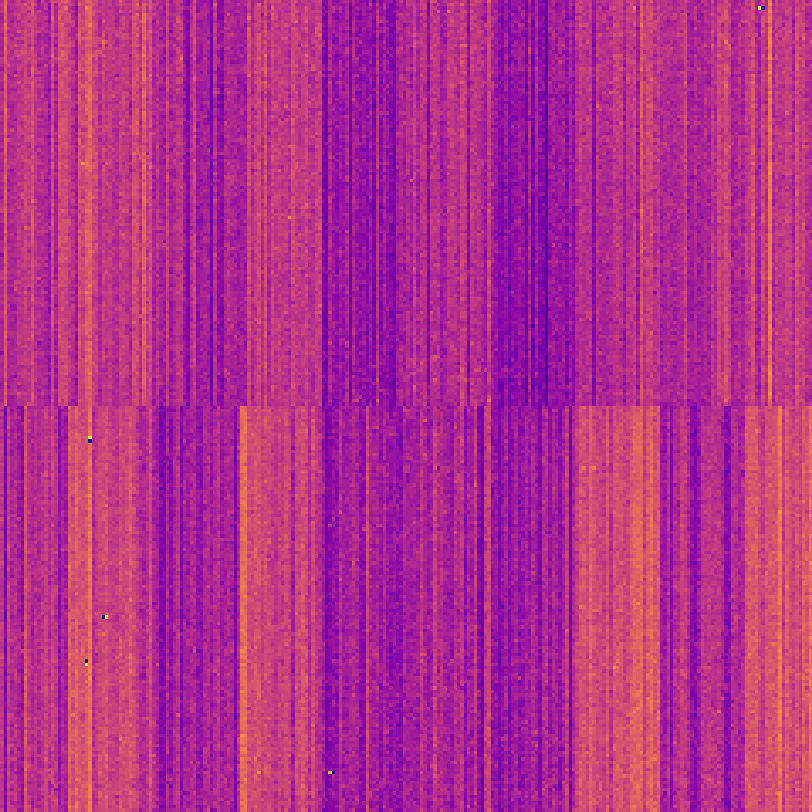
\includegraphics[interpolate=true,width=1.624000in,height=1.624000in]{capture_ped_diff-img0.png}}%
\end{pgfscope}%
\begin{pgfscope}%
\pgfsetrectcap%
\pgfsetmiterjoin%
\pgfsetlinewidth{0.803000pt}%
\definecolor{currentstroke}{rgb}{0.000000,0.000000,0.000000}%
\pgfsetstrokecolor{currentstroke}%
\pgfsetdash{}{0pt}%
\pgfpathmoveto{\pgfqpoint{0.162400in}{0.544877in}}%
\pgfpathlineto{\pgfqpoint{0.162400in}{2.168877in}}%
\pgfusepath{stroke}%
\end{pgfscope}%
\begin{pgfscope}%
\pgfsetrectcap%
\pgfsetmiterjoin%
\pgfsetlinewidth{0.803000pt}%
\definecolor{currentstroke}{rgb}{0.000000,0.000000,0.000000}%
\pgfsetstrokecolor{currentstroke}%
\pgfsetdash{}{0pt}%
\pgfpathmoveto{\pgfqpoint{1.786400in}{0.544877in}}%
\pgfpathlineto{\pgfqpoint{1.786400in}{2.168877in}}%
\pgfusepath{stroke}%
\end{pgfscope}%
\begin{pgfscope}%
\pgfsetrectcap%
\pgfsetmiterjoin%
\pgfsetlinewidth{0.803000pt}%
\definecolor{currentstroke}{rgb}{0.000000,0.000000,0.000000}%
\pgfsetstrokecolor{currentstroke}%
\pgfsetdash{}{0pt}%
\pgfpathmoveto{\pgfqpoint{0.162400in}{0.544877in}}%
\pgfpathlineto{\pgfqpoint{1.786400in}{0.544877in}}%
\pgfusepath{stroke}%
\end{pgfscope}%
\begin{pgfscope}%
\pgfsetrectcap%
\pgfsetmiterjoin%
\pgfsetlinewidth{0.803000pt}%
\definecolor{currentstroke}{rgb}{0.000000,0.000000,0.000000}%
\pgfsetstrokecolor{currentstroke}%
\pgfsetdash{}{0pt}%
\pgfpathmoveto{\pgfqpoint{0.162400in}{2.168877in}}%
\pgfpathlineto{\pgfqpoint{1.786400in}{2.168877in}}%
\pgfusepath{stroke}%
\end{pgfscope}%
\begin{pgfscope}%
\definecolor{textcolor}{rgb}{0.000000,0.000000,0.000000}%
\pgfsetstrokecolor{textcolor}%
\pgfsetfillcolor{textcolor}%
\pgftext[x=0.000000in,y=2.331277in,left,base]{\color{textcolor}\rmfamily\fontsize{10.000000}{12.000000}\selectfont (a)}%
\end{pgfscope}%
\begin{pgfscope}%
\pgfsetbuttcap%
\pgfsetmiterjoin%
\definecolor{currentfill}{rgb}{1.000000,1.000000,1.000000}%
\pgfsetfillcolor{currentfill}%
\pgfsetlinewidth{0.000000pt}%
\definecolor{currentstroke}{rgb}{0.000000,0.000000,0.000000}%
\pgfsetstrokecolor{currentstroke}%
\pgfsetstrokeopacity{0.000000}%
\pgfsetdash{}{0pt}%
\pgfpathmoveto{\pgfqpoint{1.886400in}{0.544877in}}%
\pgfpathlineto{\pgfqpoint{3.510400in}{0.544877in}}%
\pgfpathlineto{\pgfqpoint{3.510400in}{2.168877in}}%
\pgfpathlineto{\pgfqpoint{1.886400in}{2.168877in}}%
\pgfpathlineto{\pgfqpoint{1.886400in}{0.544877in}}%
\pgfpathclose%
\pgfusepath{fill}%
\end{pgfscope}%
\begin{pgfscope}%
\pgfsys@transformshift{1.886000in}{0.545419in}%
\pgftext[left,bottom]{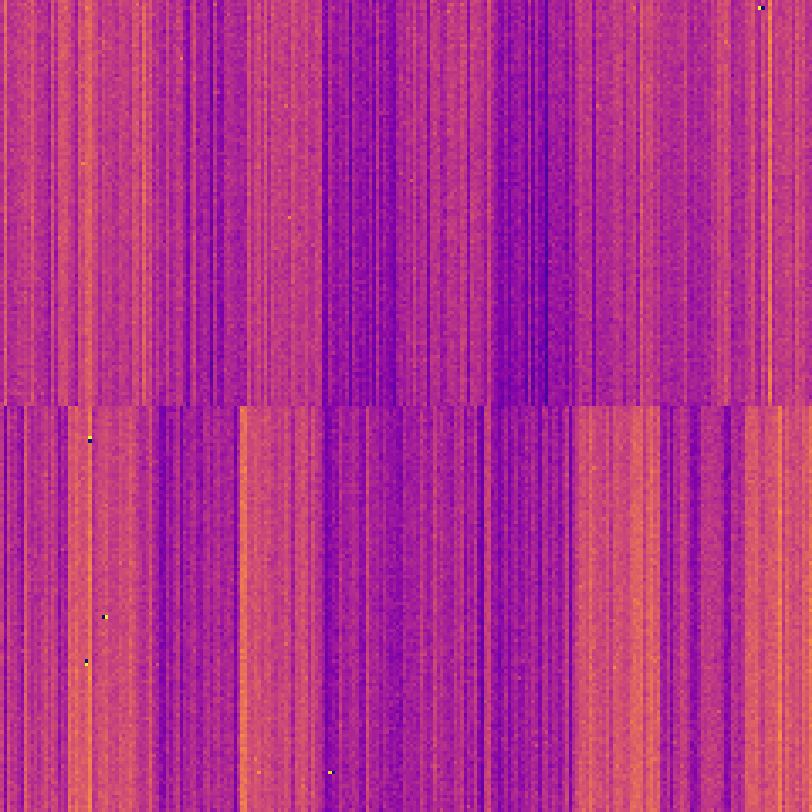
\includegraphics[interpolate=true,width=1.624000in,height=1.624000in]{capture_ped_diff-img1.png}}%
\end{pgfscope}%
\begin{pgfscope}%
\pgfsetrectcap%
\pgfsetmiterjoin%
\pgfsetlinewidth{0.803000pt}%
\definecolor{currentstroke}{rgb}{0.000000,0.000000,0.000000}%
\pgfsetstrokecolor{currentstroke}%
\pgfsetdash{}{0pt}%
\pgfpathmoveto{\pgfqpoint{1.886400in}{0.544877in}}%
\pgfpathlineto{\pgfqpoint{1.886400in}{2.168877in}}%
\pgfusepath{stroke}%
\end{pgfscope}%
\begin{pgfscope}%
\pgfsetrectcap%
\pgfsetmiterjoin%
\pgfsetlinewidth{0.803000pt}%
\definecolor{currentstroke}{rgb}{0.000000,0.000000,0.000000}%
\pgfsetstrokecolor{currentstroke}%
\pgfsetdash{}{0pt}%
\pgfpathmoveto{\pgfqpoint{3.510400in}{0.544877in}}%
\pgfpathlineto{\pgfqpoint{3.510400in}{2.168877in}}%
\pgfusepath{stroke}%
\end{pgfscope}%
\begin{pgfscope}%
\pgfsetrectcap%
\pgfsetmiterjoin%
\pgfsetlinewidth{0.803000pt}%
\definecolor{currentstroke}{rgb}{0.000000,0.000000,0.000000}%
\pgfsetstrokecolor{currentstroke}%
\pgfsetdash{}{0pt}%
\pgfpathmoveto{\pgfqpoint{1.886400in}{0.544877in}}%
\pgfpathlineto{\pgfqpoint{3.510400in}{0.544877in}}%
\pgfusepath{stroke}%
\end{pgfscope}%
\begin{pgfscope}%
\pgfsetrectcap%
\pgfsetmiterjoin%
\pgfsetlinewidth{0.803000pt}%
\definecolor{currentstroke}{rgb}{0.000000,0.000000,0.000000}%
\pgfsetstrokecolor{currentstroke}%
\pgfsetdash{}{0pt}%
\pgfpathmoveto{\pgfqpoint{1.886400in}{2.168877in}}%
\pgfpathlineto{\pgfqpoint{3.510400in}{2.168877in}}%
\pgfusepath{stroke}%
\end{pgfscope}%
\begin{pgfscope}%
\definecolor{textcolor}{rgb}{0.000000,0.000000,0.000000}%
\pgfsetstrokecolor{textcolor}%
\pgfsetfillcolor{textcolor}%
\pgftext[x=1.724000in,y=2.331277in,left,base]{\color{textcolor}\rmfamily\fontsize{10.000000}{12.000000}\selectfont (b)}%
\end{pgfscope}%
\begin{pgfscope}%
\pgfsetbuttcap%
\pgfsetmiterjoin%
\definecolor{currentfill}{rgb}{1.000000,1.000000,1.000000}%
\pgfsetfillcolor{currentfill}%
\pgfsetlinewidth{0.000000pt}%
\definecolor{currentstroke}{rgb}{0.000000,0.000000,0.000000}%
\pgfsetstrokecolor{currentstroke}%
\pgfsetstrokeopacity{0.000000}%
\pgfsetdash{}{0pt}%
\pgfpathmoveto{\pgfqpoint{0.162400in}{0.244877in}}%
\pgfpathlineto{\pgfqpoint{3.510400in}{0.244877in}}%
\pgfpathlineto{\pgfqpoint{3.510400in}{0.344877in}}%
\pgfpathlineto{\pgfqpoint{0.162400in}{0.344877in}}%
\pgfpathlineto{\pgfqpoint{0.162400in}{0.244877in}}%
\pgfpathclose%
\pgfusepath{fill}%
\end{pgfscope}%
\begin{pgfscope}%
\pgfpathrectangle{\pgfqpoint{0.162400in}{0.244877in}}{\pgfqpoint{3.348000in}{0.100000in}}%
\pgfusepath{clip}%
\pgfsetbuttcap%
\pgfsetmiterjoin%
\definecolor{currentfill}{rgb}{1.000000,1.000000,1.000000}%
\pgfsetfillcolor{currentfill}%
\pgfsetlinewidth{0.010037pt}%
\definecolor{currentstroke}{rgb}{1.000000,1.000000,1.000000}%
\pgfsetstrokecolor{currentstroke}%
\pgfsetdash{}{0pt}%
\pgfusepath{stroke,fill}%
\end{pgfscope}%
\begin{pgfscope}%
\pgfpathrectangle{\pgfqpoint{0.162400in}{0.244877in}}{\pgfqpoint{3.348000in}{0.100000in}}%
\pgfusepath{clip}%
\pgfsetbuttcap%
\pgfsetmiterjoin%
\definecolor{currentfill}{rgb}{1.000000,1.000000,1.000000}%
\pgfsetfillcolor{currentfill}%
\pgfsetlinewidth{0.010037pt}%
\definecolor{currentstroke}{rgb}{1.000000,1.000000,1.000000}%
\pgfsetstrokecolor{currentstroke}%
\pgfsetdash{}{0pt}%
\pgfusepath{stroke,fill}%
\end{pgfscope}%
\begin{pgfscope}%
\pgfsys@transformshift{0.162000in}{0.245419in}%
\pgftext[left,bottom]{
\includegraphics[interpolate=true,width=3.348000in,height=0.100000in]{capture_ped_diff-img2.png}}%
\end{pgfscope}%
\begin{pgfscope}%
\pgfsetbuttcap%
\pgfsetroundjoin%
\definecolor{currentfill}{rgb}{0.000000,0.000000,0.000000}%
\pgfsetfillcolor{currentfill}%
\pgfsetlinewidth{0.803000pt}%
\definecolor{currentstroke}{rgb}{0.000000,0.000000,0.000000}%
\pgfsetstrokecolor{currentstroke}%
\pgfsetdash{}{0pt}%
\pgfsys@defobject{currentmarker}{\pgfqpoint{0.000000in}{-0.048611in}}{\pgfqpoint{0.000000in}{0.000000in}}{%
\pgfpathmoveto{\pgfqpoint{0.000000in}{0.000000in}}%
\pgfpathlineto{\pgfqpoint{0.000000in}{-0.048611in}}%
\pgfusepath{stroke,fill}%
}%
\begin{pgfscope}%
\pgfsys@transformshift{0.162400in}{0.244877in}%
\pgfsys@useobject{currentmarker}{}%
\end{pgfscope}%
\end{pgfscope}%
\begin{pgfscope}%
\definecolor{textcolor}{rgb}{0.000000,0.000000,0.000000}%
\pgfsetstrokecolor{textcolor}%
\pgfsetfillcolor{textcolor}%
\pgftext[x=0.162400in,y=0.147655in,,top]{\color{textcolor}\rmfamily\fontsize{10.000000}{12.000000}\selectfont 5000}%
\end{pgfscope}%
\begin{pgfscope}%
\pgfsetbuttcap%
\pgfsetroundjoin%
\definecolor{currentfill}{rgb}{0.000000,0.000000,0.000000}%
\pgfsetfillcolor{currentfill}%
\pgfsetlinewidth{0.803000pt}%
\definecolor{currentstroke}{rgb}{0.000000,0.000000,0.000000}%
\pgfsetstrokecolor{currentstroke}%
\pgfsetdash{}{0pt}%
\pgfsys@defobject{currentmarker}{\pgfqpoint{0.000000in}{-0.048611in}}{\pgfqpoint{0.000000in}{0.000000in}}{%
\pgfpathmoveto{\pgfqpoint{0.000000in}{0.000000in}}%
\pgfpathlineto{\pgfqpoint{0.000000in}{-0.048611in}}%
\pgfusepath{stroke,fill}%
}%
\begin{pgfscope}%
\pgfsys@transformshift{0.832000in}{0.244877in}%
\pgfsys@useobject{currentmarker}{}%
\end{pgfscope}%
\end{pgfscope}%
\begin{pgfscope}%
\definecolor{textcolor}{rgb}{0.000000,0.000000,0.000000}%
\pgfsetstrokecolor{textcolor}%
\pgfsetfillcolor{textcolor}%
\pgftext[x=0.832000in,y=0.147655in,,top]{\color{textcolor}\rmfamily\fontsize{10.000000}{12.000000}\selectfont 5200}%
\end{pgfscope}%
\begin{pgfscope}%
\pgfsetbuttcap%
\pgfsetroundjoin%
\definecolor{currentfill}{rgb}{0.000000,0.000000,0.000000}%
\pgfsetfillcolor{currentfill}%
\pgfsetlinewidth{0.803000pt}%
\definecolor{currentstroke}{rgb}{0.000000,0.000000,0.000000}%
\pgfsetstrokecolor{currentstroke}%
\pgfsetdash{}{0pt}%
\pgfsys@defobject{currentmarker}{\pgfqpoint{0.000000in}{-0.048611in}}{\pgfqpoint{0.000000in}{0.000000in}}{%
\pgfpathmoveto{\pgfqpoint{0.000000in}{0.000000in}}%
\pgfpathlineto{\pgfqpoint{0.000000in}{-0.048611in}}%
\pgfusepath{stroke,fill}%
}%
\begin{pgfscope}%
\pgfsys@transformshift{1.501600in}{0.244877in}%
\pgfsys@useobject{currentmarker}{}%
\end{pgfscope}%
\end{pgfscope}%
\begin{pgfscope}%
\definecolor{textcolor}{rgb}{0.000000,0.000000,0.000000}%
\pgfsetstrokecolor{textcolor}%
\pgfsetfillcolor{textcolor}%
\pgftext[x=1.501600in,y=0.147655in,,top]{\color{textcolor}\rmfamily\fontsize{10.000000}{12.000000}\selectfont 5400}%
\end{pgfscope}%
\begin{pgfscope}%
\pgfsetbuttcap%
\pgfsetroundjoin%
\definecolor{currentfill}{rgb}{0.000000,0.000000,0.000000}%
\pgfsetfillcolor{currentfill}%
\pgfsetlinewidth{0.803000pt}%
\definecolor{currentstroke}{rgb}{0.000000,0.000000,0.000000}%
\pgfsetstrokecolor{currentstroke}%
\pgfsetdash{}{0pt}%
\pgfsys@defobject{currentmarker}{\pgfqpoint{0.000000in}{-0.048611in}}{\pgfqpoint{0.000000in}{0.000000in}}{%
\pgfpathmoveto{\pgfqpoint{0.000000in}{0.000000in}}%
\pgfpathlineto{\pgfqpoint{0.000000in}{-0.048611in}}%
\pgfusepath{stroke,fill}%
}%
\begin{pgfscope}%
\pgfsys@transformshift{2.171200in}{0.244877in}%
\pgfsys@useobject{currentmarker}{}%
\end{pgfscope}%
\end{pgfscope}%
\begin{pgfscope}%
\definecolor{textcolor}{rgb}{0.000000,0.000000,0.000000}%
\pgfsetstrokecolor{textcolor}%
\pgfsetfillcolor{textcolor}%
\pgftext[x=2.171200in,y=0.147655in,,top]{\color{textcolor}\rmfamily\fontsize{10.000000}{12.000000}\selectfont 5600}%
\end{pgfscope}%
\begin{pgfscope}%
\pgfsetbuttcap%
\pgfsetroundjoin%
\definecolor{currentfill}{rgb}{0.000000,0.000000,0.000000}%
\pgfsetfillcolor{currentfill}%
\pgfsetlinewidth{0.803000pt}%
\definecolor{currentstroke}{rgb}{0.000000,0.000000,0.000000}%
\pgfsetstrokecolor{currentstroke}%
\pgfsetdash{}{0pt}%
\pgfsys@defobject{currentmarker}{\pgfqpoint{0.000000in}{-0.048611in}}{\pgfqpoint{0.000000in}{0.000000in}}{%
\pgfpathmoveto{\pgfqpoint{0.000000in}{0.000000in}}%
\pgfpathlineto{\pgfqpoint{0.000000in}{-0.048611in}}%
\pgfusepath{stroke,fill}%
}%
\begin{pgfscope}%
\pgfsys@transformshift{2.840800in}{0.244877in}%
\pgfsys@useobject{currentmarker}{}%
\end{pgfscope}%
\end{pgfscope}%
\begin{pgfscope}%
\definecolor{textcolor}{rgb}{0.000000,0.000000,0.000000}%
\pgfsetstrokecolor{textcolor}%
\pgfsetfillcolor{textcolor}%
\pgftext[x=2.840800in,y=0.147655in,,top]{\color{textcolor}\rmfamily\fontsize{10.000000}{12.000000}\selectfont 5800}%
\end{pgfscope}%
\begin{pgfscope}%
\pgfsetbuttcap%
\pgfsetroundjoin%
\definecolor{currentfill}{rgb}{0.000000,0.000000,0.000000}%
\pgfsetfillcolor{currentfill}%
\pgfsetlinewidth{0.803000pt}%
\definecolor{currentstroke}{rgb}{0.000000,0.000000,0.000000}%
\pgfsetstrokecolor{currentstroke}%
\pgfsetdash{}{0pt}%
\pgfsys@defobject{currentmarker}{\pgfqpoint{0.000000in}{-0.048611in}}{\pgfqpoint{0.000000in}{0.000000in}}{%
\pgfpathmoveto{\pgfqpoint{0.000000in}{0.000000in}}%
\pgfpathlineto{\pgfqpoint{0.000000in}{-0.048611in}}%
\pgfusepath{stroke,fill}%
}%
\begin{pgfscope}%
\pgfsys@transformshift{3.510400in}{0.244877in}%
\pgfsys@useobject{currentmarker}{}%
\end{pgfscope}%
\end{pgfscope}%
\begin{pgfscope}%
\definecolor{textcolor}{rgb}{0.000000,0.000000,0.000000}%
\pgfsetstrokecolor{textcolor}%
\pgfsetfillcolor{textcolor}%
\pgftext[x=3.510400in,y=0.147655in,,top]{\color{textcolor}\rmfamily\fontsize{10.000000}{12.000000}\selectfont 6000}%
\end{pgfscope}%
\begin{pgfscope}%
\pgfsetrectcap%
\pgfsetmiterjoin%
\pgfsetlinewidth{0.803000pt}%
\definecolor{currentstroke}{rgb}{0.000000,0.000000,0.000000}%
\pgfsetstrokecolor{currentstroke}%
\pgfsetdash{}{0pt}%
\pgfpathmoveto{\pgfqpoint{0.162400in}{0.244877in}}%
\pgfpathlineto{\pgfqpoint{0.162400in}{0.294877in}}%
\pgfpathlineto{\pgfqpoint{0.162400in}{0.344877in}}%
\pgfpathlineto{\pgfqpoint{3.510400in}{0.344877in}}%
\pgfpathlineto{\pgfqpoint{3.510400in}{0.294877in}}%
\pgfpathlineto{\pgfqpoint{3.510400in}{0.244877in}}%
\pgfpathlineto{\pgfqpoint{0.162400in}{0.244877in}}%
\pgfpathclose%
\pgfusepath{stroke}%
\end{pgfscope}%
\begin{pgfscope}%
\pgfsetbuttcap%
\pgfsetmiterjoin%
\pgfsetlinewidth{0.000000pt}%
\definecolor{currentstroke}{rgb}{1.000000,1.000000,1.000000}%
\pgfsetstrokecolor{currentstroke}%
\pgfsetstrokeopacity{0.000000}%
\pgfsetdash{}{0pt}%
\pgfpathmoveto{\pgfqpoint{3.942400in}{-1.556873in}}%
\pgfpathlineto{\pgfqpoint{6.102400in}{-1.556873in}}%
\pgfpathlineto{\pgfqpoint{6.102400in}{3.943127in}}%
\pgfpathlineto{\pgfqpoint{3.942400in}{3.943127in}}%
\pgfpathlineto{\pgfqpoint{3.942400in}{-1.556873in}}%
\pgfpathclose%
\pgfusepath{}%
\end{pgfscope}%
\begin{pgfscope}%
\pgfsetbuttcap%
\pgfsetmiterjoin%
\definecolor{currentfill}{rgb}{1.000000,1.000000,1.000000}%
\pgfsetfillcolor{currentfill}%
\pgfsetlinewidth{0.000000pt}%
\definecolor{currentstroke}{rgb}{0.000000,0.000000,0.000000}%
\pgfsetstrokecolor{currentstroke}%
\pgfsetstrokeopacity{0.000000}%
\pgfsetdash{}{0pt}%
\pgfpathmoveto{\pgfqpoint{4.212400in}{0.519877in}}%
\pgfpathlineto{\pgfqpoint{5.886400in}{0.519877in}}%
\pgfpathlineto{\pgfqpoint{5.886400in}{2.193877in}}%
\pgfpathlineto{\pgfqpoint{4.212400in}{2.193877in}}%
\pgfpathlineto{\pgfqpoint{4.212400in}{0.519877in}}%
\pgfpathclose%
\pgfusepath{fill}%
\end{pgfscope}%
\begin{pgfscope}%
\pgfsys@transformshift{4.212000in}{0.521419in}%
\pgftext[left,bottom]{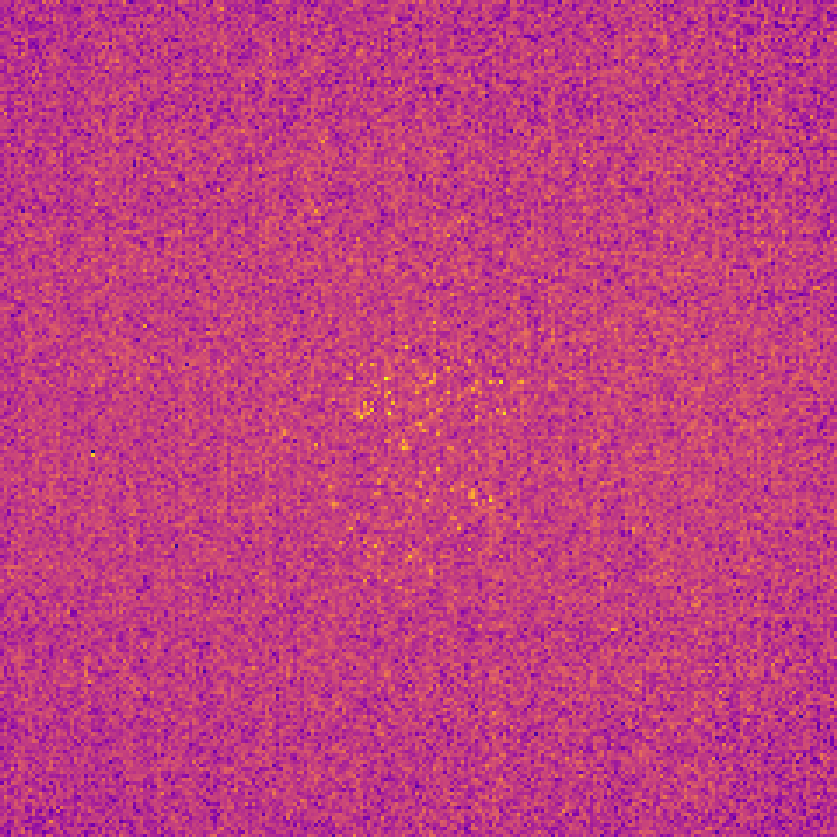
\includegraphics[interpolate=true,width=1.674000in,height=1.674000in]{capture_ped_diff-img3.png}}%
\end{pgfscope}%
\begin{pgfscope}%
\pgfsetrectcap%
\pgfsetmiterjoin%
\pgfsetlinewidth{0.803000pt}%
\definecolor{currentstroke}{rgb}{0.000000,0.000000,0.000000}%
\pgfsetstrokecolor{currentstroke}%
\pgfsetdash{}{0pt}%
\pgfpathmoveto{\pgfqpoint{4.212400in}{0.519877in}}%
\pgfpathlineto{\pgfqpoint{4.212400in}{2.193877in}}%
\pgfusepath{stroke}%
\end{pgfscope}%
\begin{pgfscope}%
\pgfsetrectcap%
\pgfsetmiterjoin%
\pgfsetlinewidth{0.803000pt}%
\definecolor{currentstroke}{rgb}{0.000000,0.000000,0.000000}%
\pgfsetstrokecolor{currentstroke}%
\pgfsetdash{}{0pt}%
\pgfpathmoveto{\pgfqpoint{5.886400in}{0.519877in}}%
\pgfpathlineto{\pgfqpoint{5.886400in}{2.193877in}}%
\pgfusepath{stroke}%
\end{pgfscope}%
\begin{pgfscope}%
\pgfsetrectcap%
\pgfsetmiterjoin%
\pgfsetlinewidth{0.803000pt}%
\definecolor{currentstroke}{rgb}{0.000000,0.000000,0.000000}%
\pgfsetstrokecolor{currentstroke}%
\pgfsetdash{}{0pt}%
\pgfpathmoveto{\pgfqpoint{4.212400in}{0.519877in}}%
\pgfpathlineto{\pgfqpoint{5.886400in}{0.519877in}}%
\pgfusepath{stroke}%
\end{pgfscope}%
\begin{pgfscope}%
\pgfsetrectcap%
\pgfsetmiterjoin%
\pgfsetlinewidth{0.803000pt}%
\definecolor{currentstroke}{rgb}{0.000000,0.000000,0.000000}%
\pgfsetstrokecolor{currentstroke}%
\pgfsetdash{}{0pt}%
\pgfpathmoveto{\pgfqpoint{4.212400in}{2.193877in}}%
\pgfpathlineto{\pgfqpoint{5.886400in}{2.193877in}}%
\pgfusepath{stroke}%
\end{pgfscope}%
\begin{pgfscope}%
\definecolor{textcolor}{rgb}{0.000000,0.000000,0.000000}%
\pgfsetstrokecolor{textcolor}%
\pgfsetfillcolor{textcolor}%
\pgftext[x=4.045000in,y=2.361277in,left,base]{\color{textcolor}\rmfamily\fontsize{10.000000}{12.000000}\selectfont (c)}%
\end{pgfscope}%
\begin{pgfscope}%
\pgfsetbuttcap%
\pgfsetmiterjoin%
\definecolor{currentfill}{rgb}{1.000000,1.000000,1.000000}%
\pgfsetfillcolor{currentfill}%
\pgfsetlinewidth{0.000000pt}%
\definecolor{currentstroke}{rgb}{0.000000,0.000000,0.000000}%
\pgfsetstrokecolor{currentstroke}%
\pgfsetstrokeopacity{0.000000}%
\pgfsetdash{}{0pt}%
\pgfpathmoveto{\pgfqpoint{4.212400in}{0.219877in}}%
\pgfpathlineto{\pgfqpoint{5.886400in}{0.219877in}}%
\pgfpathlineto{\pgfqpoint{5.886400in}{0.319877in}}%
\pgfpathlineto{\pgfqpoint{4.212400in}{0.319877in}}%
\pgfpathlineto{\pgfqpoint{4.212400in}{0.219877in}}%
\pgfpathclose%
\pgfusepath{fill}%
\end{pgfscope}%
\begin{pgfscope}%
\pgfpathrectangle{\pgfqpoint{4.212400in}{0.219877in}}{\pgfqpoint{1.674000in}{0.100000in}}%
\pgfusepath{clip}%
\pgfsetbuttcap%
\pgfsetmiterjoin%
\definecolor{currentfill}{rgb}{1.000000,1.000000,1.000000}%
\pgfsetfillcolor{currentfill}%
\pgfsetlinewidth{0.010037pt}%
\definecolor{currentstroke}{rgb}{1.000000,1.000000,1.000000}%
\pgfsetstrokecolor{currentstroke}%
\pgfsetdash{}{0pt}%
\pgfusepath{stroke,fill}%
\end{pgfscope}%
\begin{pgfscope}%
\pgfsys@transformshift{4.212000in}{0.221419in}%
\pgftext[left,bottom]{
\includegraphics[interpolate=true,width=1.674000in,height=0.100000in]{capture_ped_diff-img4.png}}%
\end{pgfscope}%
\begin{pgfscope}%
\pgfsetbuttcap%
\pgfsetroundjoin%
\definecolor{currentfill}{rgb}{0.000000,0.000000,0.000000}%
\pgfsetfillcolor{currentfill}%
\pgfsetlinewidth{0.803000pt}%
\definecolor{currentstroke}{rgb}{0.000000,0.000000,0.000000}%
\pgfsetstrokecolor{currentstroke}%
\pgfsetdash{}{0pt}%
\pgfsys@defobject{currentmarker}{\pgfqpoint{0.000000in}{-0.048611in}}{\pgfqpoint{0.000000in}{0.000000in}}{%
\pgfpathmoveto{\pgfqpoint{0.000000in}{0.000000in}}%
\pgfpathlineto{\pgfqpoint{0.000000in}{-0.048611in}}%
\pgfusepath{stroke,fill}%
}%
\begin{pgfscope}%
\pgfsys@transformshift{4.507224in}{0.219877in}%
\pgfsys@useobject{currentmarker}{}%
\end{pgfscope}%
\end{pgfscope}%
\begin{pgfscope}%
\definecolor{textcolor}{rgb}{0.000000,0.000000,0.000000}%
\pgfsetstrokecolor{textcolor}%
\pgfsetfillcolor{textcolor}%
\pgftext[x=4.507224in,y=0.122655in,,top]{\color{textcolor}\rmfamily\fontsize{10.000000}{12.000000}\selectfont -100}%
\end{pgfscope}%
\begin{pgfscope}%
\pgfsetbuttcap%
\pgfsetroundjoin%
\definecolor{currentfill}{rgb}{0.000000,0.000000,0.000000}%
\pgfsetfillcolor{currentfill}%
\pgfsetlinewidth{0.803000pt}%
\definecolor{currentstroke}{rgb}{0.000000,0.000000,0.000000}%
\pgfsetstrokecolor{currentstroke}%
\pgfsetdash{}{0pt}%
\pgfsys@defobject{currentmarker}{\pgfqpoint{0.000000in}{-0.048611in}}{\pgfqpoint{0.000000in}{0.000000in}}{%
\pgfpathmoveto{\pgfqpoint{0.000000in}{0.000000in}}%
\pgfpathlineto{\pgfqpoint{0.000000in}{-0.048611in}}%
\pgfusepath{stroke,fill}%
}%
\begin{pgfscope}%
\pgfsys@transformshift{5.006925in}{0.219877in}%
\pgfsys@useobject{currentmarker}{}%
\end{pgfscope}%
\end{pgfscope}%
\begin{pgfscope}%
\definecolor{textcolor}{rgb}{0.000000,0.000000,0.000000}%
\pgfsetstrokecolor{textcolor}%
\pgfsetfillcolor{textcolor}%
\pgftext[x=5.006925in,y=0.122655in,,top]{\color{textcolor}\rmfamily\fontsize{10.000000}{12.000000}\selectfont 0}%
\end{pgfscope}%
\begin{pgfscope}%
\pgfsetbuttcap%
\pgfsetroundjoin%
\definecolor{currentfill}{rgb}{0.000000,0.000000,0.000000}%
\pgfsetfillcolor{currentfill}%
\pgfsetlinewidth{0.803000pt}%
\definecolor{currentstroke}{rgb}{0.000000,0.000000,0.000000}%
\pgfsetstrokecolor{currentstroke}%
\pgfsetdash{}{0pt}%
\pgfsys@defobject{currentmarker}{\pgfqpoint{0.000000in}{-0.048611in}}{\pgfqpoint{0.000000in}{0.000000in}}{%
\pgfpathmoveto{\pgfqpoint{0.000000in}{0.000000in}}%
\pgfpathlineto{\pgfqpoint{0.000000in}{-0.048611in}}%
\pgfusepath{stroke,fill}%
}%
\begin{pgfscope}%
\pgfsys@transformshift{5.506627in}{0.219877in}%
\pgfsys@useobject{currentmarker}{}%
\end{pgfscope}%
\end{pgfscope}%
\begin{pgfscope}%
\definecolor{textcolor}{rgb}{0.000000,0.000000,0.000000}%
\pgfsetstrokecolor{textcolor}%
\pgfsetfillcolor{textcolor}%
\pgftext[x=5.506627in,y=0.122655in,,top]{\color{textcolor}\rmfamily\fontsize{10.000000}{12.000000}\selectfont 100}%
\end{pgfscope}%
\begin{pgfscope}%
\pgfsetrectcap%
\pgfsetmiterjoin%
\pgfsetlinewidth{0.803000pt}%
\definecolor{currentstroke}{rgb}{0.000000,0.000000,0.000000}%
\pgfsetstrokecolor{currentstroke}%
\pgfsetdash{}{0pt}%
\pgfpathmoveto{\pgfqpoint{4.212400in}{0.219877in}}%
\pgfpathlineto{\pgfqpoint{4.212400in}{0.269877in}}%
\pgfpathlineto{\pgfqpoint{4.212400in}{0.319877in}}%
\pgfpathlineto{\pgfqpoint{5.886400in}{0.319877in}}%
\pgfpathlineto{\pgfqpoint{5.886400in}{0.269877in}}%
\pgfpathlineto{\pgfqpoint{5.886400in}{0.219877in}}%
\pgfpathlineto{\pgfqpoint{4.212400in}{0.219877in}}%
\pgfpathclose%
\pgfusepath{stroke}%
\end{pgfscope}%
\end{pgfpicture}%
\makeatother%
\endgroup%

    \caption{(a) eine Einzelaufnahme der gestreuten Photonen, (b) ein gemitteltes Bild über \num{10000} Dunkelbilder und (c) die resultierende Differenz von ersten zwei Bildern.}
    \label{fig:capture_ped_diff}
\end{figure}

\noindent
Bei jedem Auswertungsvorgang werden die beiden Algorithmen (Abschnitte \ref{text:threshold_algorithm} und \ref{text:clustering_algorithm}) eingesetzt und die Auswertungsergebnisse werden miteinander verglichen.
\section{Hintergrundrauschen Auswertung der Streubilder}
\label{text:streuung_counting}
Die Messdaten wurden zuerst mit dem Schwellenwert-Algorithmus verarbeitet, wobei diverse Werte aus dem Intervall \SIrange{150}{600}{\adu} dem Schwellenwert $s_V$ zugewiesen werden. Die Zahl der detektierten Photonen mit dem variablen Schwellenwert lässt quantitativ anschauen, wie stark der erwartete \gls{adu}-Wert eines Photons $W_\text{Gd, M5} =  \SI{180(1)}{\adu}$ (s. Gl. (\ref{eq:auselesewerte_fe_gd})).

\noindent
In der Abb. \ref{fig:th_150_170_180} es ist 
\begin{figure}[H]
    \centering
    %% Creator: Matplotlib, PGF backend
%%
%% To include the figure in your LaTeX document, write
%%   \input{<filename>.pgf}
%%
%% Make sure the required packages are loaded in your preamble
%%   \usepackage{pgf}
%%
%% Also ensure that all the required font packages are loaded; for instance,
%% the lmodern package is sometimes necessary when using math font.
%%   \usepackage{lmodern}
%%
%% Figures using additional raster images can only be included by \input if
%% they are in the same directory as the main LaTeX file. For loading figures
%% from other directories you can use the `import` package
%%   \usepackage{import}
%%
%% and then include the figures with
%%   \import{<path to file>}{<filename>.pgf}
%%
%% Matplotlib used the following preamble
%%   \usepackage[utf8]{inputenc} \usepackage[T1]{fontenc} \usepackage[ngerman]{babel} \usepackage{hyperref} \usepackage[sorting=none]{biblatex} \usepackage{amsmath} \usepackage[output-decimal-marker={,}]{siunitx} \sisetup{per-mode=fraction, separate-uncertainty = true, locale = DE} \usepackage[acronym, toc, section=section, nonumberlist, nopostdot]{glossaries-extra} \usepackage{lmodern}
%%
\begingroup%
\makeatletter%
\begin{pgfpicture}%
\pgfpathrectangle{\pgfpointorigin}{\pgfqpoint{6.180778in}{2.415757in}}%
\pgfusepath{use as bounding box, clip}%
\begin{pgfscope}%
\pgfsetbuttcap%
\pgfsetmiterjoin%
\pgfsetlinewidth{0.000000pt}%
\definecolor{currentstroke}{rgb}{1.000000,1.000000,1.000000}%
\pgfsetstrokecolor{currentstroke}%
\pgfsetstrokeopacity{0.000000}%
\pgfsetdash{}{0pt}%
\pgfpathmoveto{\pgfqpoint{0.000000in}{0.000000in}}%
\pgfpathlineto{\pgfqpoint{6.180778in}{0.000000in}}%
\pgfpathlineto{\pgfqpoint{6.180778in}{2.415757in}}%
\pgfpathlineto{\pgfqpoint{0.000000in}{2.415757in}}%
\pgfpathlineto{\pgfqpoint{0.000000in}{0.000000in}}%
\pgfpathclose%
\pgfusepath{}%
\end{pgfscope}%
\begin{pgfscope}%
\pgfsetbuttcap%
\pgfsetmiterjoin%
\definecolor{currentfill}{rgb}{1.000000,1.000000,1.000000}%
\pgfsetfillcolor{currentfill}%
\pgfsetlinewidth{0.000000pt}%
\definecolor{currentstroke}{rgb}{0.000000,0.000000,0.000000}%
\pgfsetstrokecolor{currentstroke}%
\pgfsetstrokeopacity{0.000000}%
\pgfsetdash{}{0pt}%
\pgfpathmoveto{\pgfqpoint{0.048611in}{0.061342in}}%
\pgfpathlineto{\pgfqpoint{1.848810in}{0.061342in}}%
\pgfpathlineto{\pgfqpoint{1.848810in}{1.861541in}}%
\pgfpathlineto{\pgfqpoint{0.048611in}{1.861541in}}%
\pgfpathlineto{\pgfqpoint{0.048611in}{0.061342in}}%
\pgfpathclose%
\pgfusepath{fill}%
\end{pgfscope}%
\begin{pgfscope}%
\pgfsys@transformshift{0.048000in}{0.063757in}%
\pgftext[left,bottom]{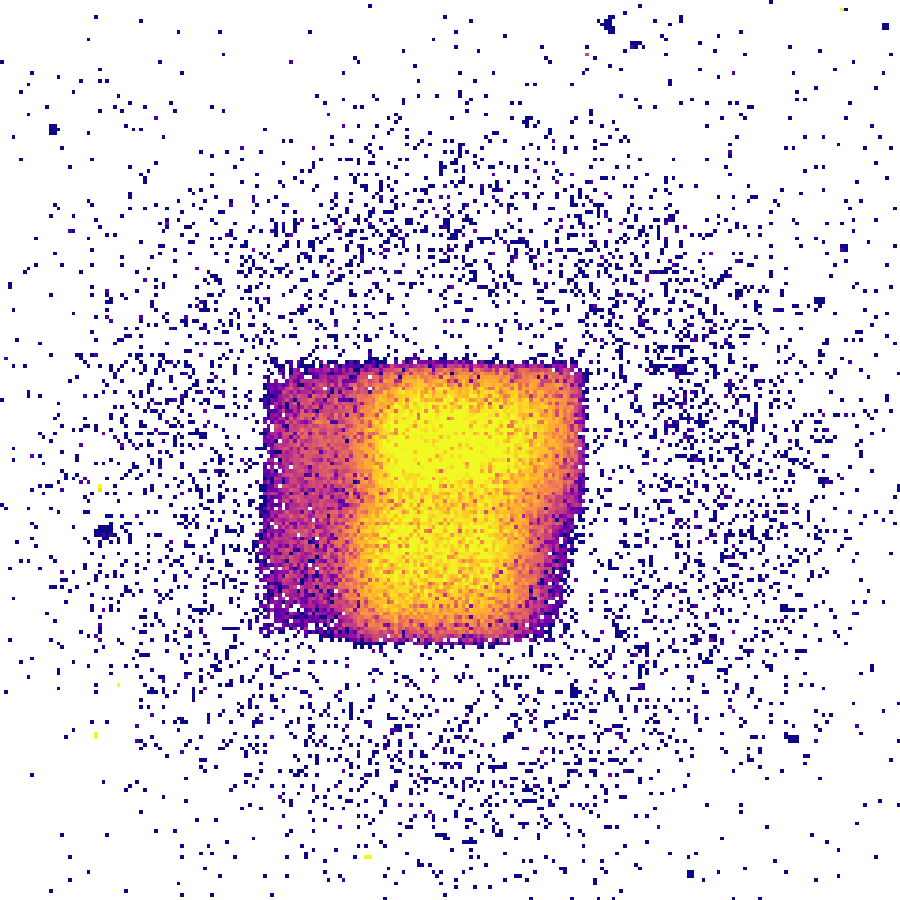
\includegraphics[interpolate=true,width=1.800000in,height=1.800000in]{th_150_170_180-img0.png}}%
\end{pgfscope}%
\begin{pgfscope}%
\pgfsetrectcap%
\pgfsetmiterjoin%
\pgfsetlinewidth{0.803000pt}%
\definecolor{currentstroke}{rgb}{0.000000,0.000000,0.000000}%
\pgfsetstrokecolor{currentstroke}%
\pgfsetdash{}{0pt}%
\pgfpathmoveto{\pgfqpoint{0.048611in}{0.061342in}}%
\pgfpathlineto{\pgfqpoint{0.048611in}{1.861541in}}%
\pgfusepath{stroke}%
\end{pgfscope}%
\begin{pgfscope}%
\pgfsetrectcap%
\pgfsetmiterjoin%
\pgfsetlinewidth{0.803000pt}%
\definecolor{currentstroke}{rgb}{0.000000,0.000000,0.000000}%
\pgfsetstrokecolor{currentstroke}%
\pgfsetdash{}{0pt}%
\pgfpathmoveto{\pgfqpoint{1.848810in}{0.061342in}}%
\pgfpathlineto{\pgfqpoint{1.848810in}{1.861541in}}%
\pgfusepath{stroke}%
\end{pgfscope}%
\begin{pgfscope}%
\pgfsetrectcap%
\pgfsetmiterjoin%
\pgfsetlinewidth{0.803000pt}%
\definecolor{currentstroke}{rgb}{0.000000,0.000000,0.000000}%
\pgfsetstrokecolor{currentstroke}%
\pgfsetdash{}{0pt}%
\pgfpathmoveto{\pgfqpoint{0.048611in}{0.061342in}}%
\pgfpathlineto{\pgfqpoint{1.848810in}{0.061342in}}%
\pgfusepath{stroke}%
\end{pgfscope}%
\begin{pgfscope}%
\pgfsetrectcap%
\pgfsetmiterjoin%
\pgfsetlinewidth{0.803000pt}%
\definecolor{currentstroke}{rgb}{0.000000,0.000000,0.000000}%
\pgfsetstrokecolor{currentstroke}%
\pgfsetdash{}{0pt}%
\pgfpathmoveto{\pgfqpoint{0.048611in}{1.861541in}}%
\pgfpathlineto{\pgfqpoint{1.848810in}{1.861541in}}%
\pgfusepath{stroke}%
\end{pgfscope}%
\begin{pgfscope}%
\definecolor{textcolor}{rgb}{0.000000,0.000000,0.000000}%
\pgfsetstrokecolor{textcolor}%
\pgfsetfillcolor{textcolor}%
\pgftext[x=0.048611in,y=2.311591in,left,base]{\color{textcolor}\rmfamily\fontsize{10.000000}{12.000000}\selectfont (a)}%
\end{pgfscope}%
\begin{pgfscope}%
\pgfsetbuttcap%
\pgfsetmiterjoin%
\definecolor{currentfill}{rgb}{1.000000,1.000000,1.000000}%
\pgfsetfillcolor{currentfill}%
\pgfsetlinewidth{0.000000pt}%
\definecolor{currentstroke}{rgb}{0.000000,0.000000,0.000000}%
\pgfsetstrokecolor{currentstroke}%
\pgfsetstrokeopacity{0.000000}%
\pgfsetdash{}{0pt}%
\pgfpathmoveto{\pgfqpoint{1.948810in}{0.061342in}}%
\pgfpathlineto{\pgfqpoint{3.749010in}{0.061342in}}%
\pgfpathlineto{\pgfqpoint{3.749010in}{1.861541in}}%
\pgfpathlineto{\pgfqpoint{1.948810in}{1.861541in}}%
\pgfpathlineto{\pgfqpoint{1.948810in}{0.061342in}}%
\pgfpathclose%
\pgfusepath{fill}%
\end{pgfscope}%
\begin{pgfscope}%
\pgfsys@transformshift{1.948000in}{0.063757in}%
\pgftext[left,bottom]{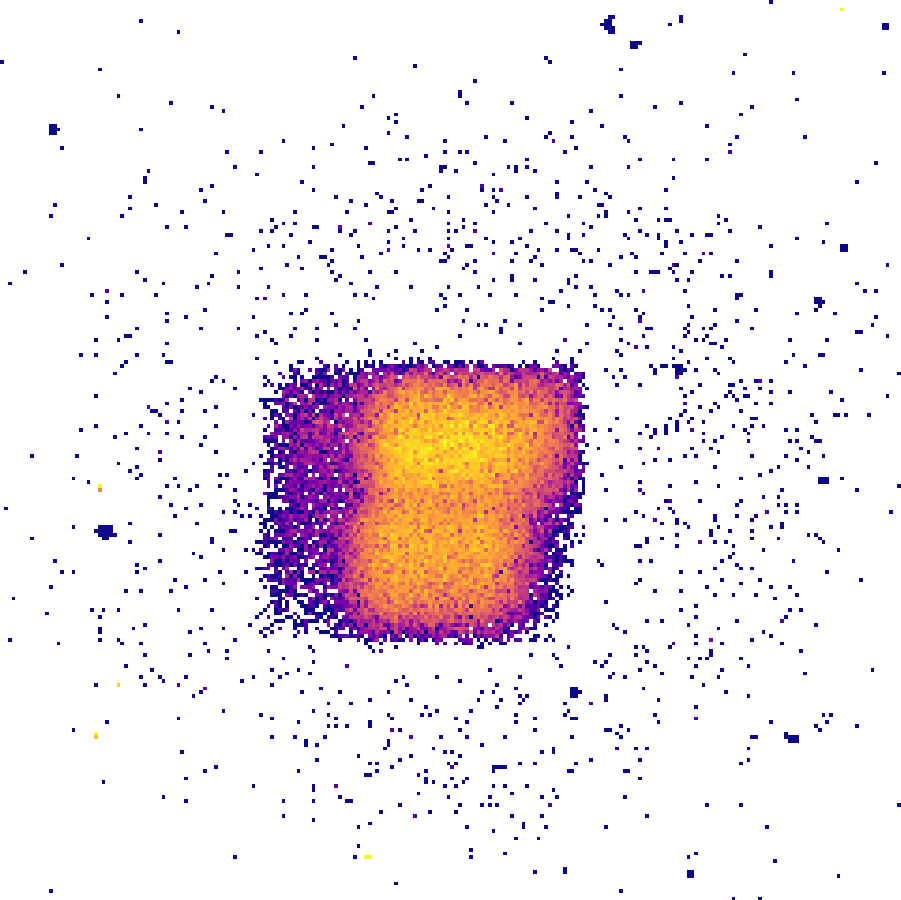
\includegraphics[interpolate=true,width=1.802000in,height=1.800000in]{th_150_170_180-img1.png}}%
\end{pgfscope}%
\begin{pgfscope}%
\pgfsetrectcap%
\pgfsetmiterjoin%
\pgfsetlinewidth{0.803000pt}%
\definecolor{currentstroke}{rgb}{0.000000,0.000000,0.000000}%
\pgfsetstrokecolor{currentstroke}%
\pgfsetdash{}{0pt}%
\pgfpathmoveto{\pgfqpoint{1.948810in}{0.061342in}}%
\pgfpathlineto{\pgfqpoint{1.948810in}{1.861541in}}%
\pgfusepath{stroke}%
\end{pgfscope}%
\begin{pgfscope}%
\pgfsetrectcap%
\pgfsetmiterjoin%
\pgfsetlinewidth{0.803000pt}%
\definecolor{currentstroke}{rgb}{0.000000,0.000000,0.000000}%
\pgfsetstrokecolor{currentstroke}%
\pgfsetdash{}{0pt}%
\pgfpathmoveto{\pgfqpoint{3.749010in}{0.061342in}}%
\pgfpathlineto{\pgfqpoint{3.749010in}{1.861541in}}%
\pgfusepath{stroke}%
\end{pgfscope}%
\begin{pgfscope}%
\pgfsetrectcap%
\pgfsetmiterjoin%
\pgfsetlinewidth{0.803000pt}%
\definecolor{currentstroke}{rgb}{0.000000,0.000000,0.000000}%
\pgfsetstrokecolor{currentstroke}%
\pgfsetdash{}{0pt}%
\pgfpathmoveto{\pgfqpoint{1.948810in}{0.061342in}}%
\pgfpathlineto{\pgfqpoint{3.749010in}{0.061342in}}%
\pgfusepath{stroke}%
\end{pgfscope}%
\begin{pgfscope}%
\pgfsetrectcap%
\pgfsetmiterjoin%
\pgfsetlinewidth{0.803000pt}%
\definecolor{currentstroke}{rgb}{0.000000,0.000000,0.000000}%
\pgfsetstrokecolor{currentstroke}%
\pgfsetdash{}{0pt}%
\pgfpathmoveto{\pgfqpoint{1.948810in}{1.861541in}}%
\pgfpathlineto{\pgfqpoint{3.749010in}{1.861541in}}%
\pgfusepath{stroke}%
\end{pgfscope}%
\begin{pgfscope}%
\definecolor{textcolor}{rgb}{0.000000,0.000000,0.000000}%
\pgfsetstrokecolor{textcolor}%
\pgfsetfillcolor{textcolor}%
\pgftext[x=1.948810in,y=2.311591in,left,base]{\color{textcolor}\rmfamily\fontsize{10.000000}{12.000000}\selectfont (b)}%
\end{pgfscope}%
\begin{pgfscope}%
\pgfsetbuttcap%
\pgfsetmiterjoin%
\definecolor{currentfill}{rgb}{1.000000,1.000000,1.000000}%
\pgfsetfillcolor{currentfill}%
\pgfsetlinewidth{0.000000pt}%
\definecolor{currentstroke}{rgb}{0.000000,0.000000,0.000000}%
\pgfsetstrokecolor{currentstroke}%
\pgfsetstrokeopacity{0.000000}%
\pgfsetdash{}{0pt}%
\pgfpathmoveto{\pgfqpoint{3.849010in}{0.061342in}}%
\pgfpathlineto{\pgfqpoint{5.649209in}{0.061342in}}%
\pgfpathlineto{\pgfqpoint{5.649209in}{1.861541in}}%
\pgfpathlineto{\pgfqpoint{3.849010in}{1.861541in}}%
\pgfpathlineto{\pgfqpoint{3.849010in}{0.061342in}}%
\pgfpathclose%
\pgfusepath{fill}%
\end{pgfscope}%
\begin{pgfscope}%
\pgfsys@transformshift{3.946000in}{0.063757in}%
\pgftext[left,bottom]{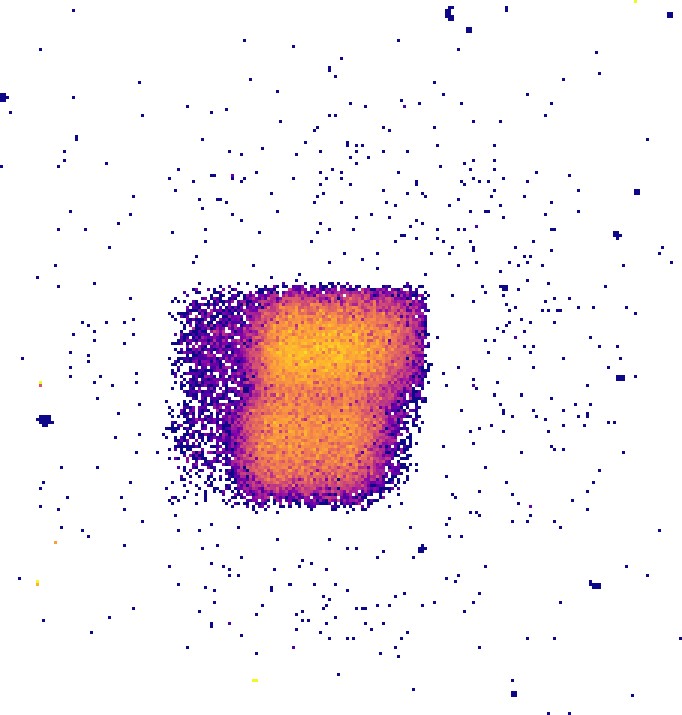
\includegraphics[interpolate=true,width=1.704000in,height=1.784000in]{th_150_170_180-img2.png}}%
\end{pgfscope}%
\begin{pgfscope}%
\pgfsetrectcap%
\pgfsetmiterjoin%
\pgfsetlinewidth{0.803000pt}%
\definecolor{currentstroke}{rgb}{0.000000,0.000000,0.000000}%
\pgfsetstrokecolor{currentstroke}%
\pgfsetdash{}{0pt}%
\pgfpathmoveto{\pgfqpoint{3.849010in}{0.061342in}}%
\pgfpathlineto{\pgfqpoint{3.849010in}{1.861541in}}%
\pgfusepath{stroke}%
\end{pgfscope}%
\begin{pgfscope}%
\pgfsetrectcap%
\pgfsetmiterjoin%
\pgfsetlinewidth{0.803000pt}%
\definecolor{currentstroke}{rgb}{0.000000,0.000000,0.000000}%
\pgfsetstrokecolor{currentstroke}%
\pgfsetdash{}{0pt}%
\pgfpathmoveto{\pgfqpoint{5.649209in}{0.061342in}}%
\pgfpathlineto{\pgfqpoint{5.649209in}{1.861541in}}%
\pgfusepath{stroke}%
\end{pgfscope}%
\begin{pgfscope}%
\pgfsetrectcap%
\pgfsetmiterjoin%
\pgfsetlinewidth{0.803000pt}%
\definecolor{currentstroke}{rgb}{0.000000,0.000000,0.000000}%
\pgfsetstrokecolor{currentstroke}%
\pgfsetdash{}{0pt}%
\pgfpathmoveto{\pgfqpoint{3.849010in}{0.061342in}}%
\pgfpathlineto{\pgfqpoint{5.649209in}{0.061342in}}%
\pgfusepath{stroke}%
\end{pgfscope}%
\begin{pgfscope}%
\pgfsetrectcap%
\pgfsetmiterjoin%
\pgfsetlinewidth{0.803000pt}%
\definecolor{currentstroke}{rgb}{0.000000,0.000000,0.000000}%
\pgfsetstrokecolor{currentstroke}%
\pgfsetdash{}{0pt}%
\pgfpathmoveto{\pgfqpoint{3.849010in}{1.861541in}}%
\pgfpathlineto{\pgfqpoint{5.649209in}{1.861541in}}%
\pgfusepath{stroke}%
\end{pgfscope}%
\begin{pgfscope}%
\definecolor{textcolor}{rgb}{0.000000,0.000000,0.000000}%
\pgfsetstrokecolor{textcolor}%
\pgfsetfillcolor{textcolor}%
\pgftext[x=3.849010in,y=2.311591in,left,base]{\color{textcolor}\rmfamily\fontsize{10.000000}{12.000000}\selectfont (c)}%
\end{pgfscope}%
\begin{pgfscope}%
\pgfsetbuttcap%
\pgfsetmiterjoin%
\definecolor{currentfill}{rgb}{1.000000,1.000000,1.000000}%
\pgfsetfillcolor{currentfill}%
\pgfsetlinewidth{0.000000pt}%
\definecolor{currentstroke}{rgb}{0.000000,0.000000,0.000000}%
\pgfsetstrokecolor{currentstroke}%
\pgfsetstrokeopacity{0.000000}%
\pgfsetdash{}{0pt}%
\pgfpathmoveto{\pgfqpoint{5.749209in}{0.061342in}}%
\pgfpathlineto{\pgfqpoint{5.875223in}{0.061342in}}%
\pgfpathlineto{\pgfqpoint{5.875223in}{1.861541in}}%
\pgfpathlineto{\pgfqpoint{5.749209in}{1.861541in}}%
\pgfpathlineto{\pgfqpoint{5.749209in}{0.061342in}}%
\pgfpathclose%
\pgfusepath{fill}%
\end{pgfscope}%
\begin{pgfscope}%
\pgfpathrectangle{\pgfqpoint{5.749209in}{0.061342in}}{\pgfqpoint{0.126014in}{1.800199in}}%
\pgfusepath{clip}%
\pgfsetbuttcap%
\pgfsetmiterjoin%
\definecolor{currentfill}{rgb}{1.000000,1.000000,1.000000}%
\pgfsetfillcolor{currentfill}%
\pgfsetlinewidth{0.010037pt}%
\definecolor{currentstroke}{rgb}{1.000000,1.000000,1.000000}%
\pgfsetstrokecolor{currentstroke}%
\pgfsetdash{}{0pt}%
\pgfusepath{stroke,fill}%
\end{pgfscope}%
\begin{pgfscope}%
\pgfsys@transformshift{5.750000in}{0.063757in}%
\pgftext[left,bottom]{
\includegraphics[interpolate=true,width=0.126000in,height=1.800000in]{th_150_170_180-img3.png}}%
\end{pgfscope}%
\begin{pgfscope}%
\pgfsetbuttcap%
\pgfsetroundjoin%
\definecolor{currentfill}{rgb}{0.000000,0.000000,0.000000}%
\pgfsetfillcolor{currentfill}%
\pgfsetlinewidth{0.803000pt}%
\definecolor{currentstroke}{rgb}{0.000000,0.000000,0.000000}%
\pgfsetstrokecolor{currentstroke}%
\pgfsetdash{}{0pt}%
\pgfsys@defobject{currentmarker}{\pgfqpoint{0.000000in}{0.000000in}}{\pgfqpoint{0.048611in}{0.000000in}}{%
\pgfpathmoveto{\pgfqpoint{0.000000in}{0.000000in}}%
\pgfpathlineto{\pgfqpoint{0.048611in}{0.000000in}}%
\pgfusepath{stroke,fill}%
}%
\begin{pgfscope}%
\pgfsys@transformshift{5.875223in}{0.061342in}%
\pgfsys@useobject{currentmarker}{}%
\end{pgfscope}%
\end{pgfscope}%
\begin{pgfscope}%
\definecolor{textcolor}{rgb}{0.000000,0.000000,0.000000}%
\pgfsetstrokecolor{textcolor}%
\pgfsetfillcolor{textcolor}%
\pgftext[x=5.972445in,y=0.061342in,left,]{\color{textcolor}\rmfamily\fontsize{10.000000}{12.000000}\selectfont 1}%
\end{pgfscope}%
\begin{pgfscope}%
\pgfsetbuttcap%
\pgfsetroundjoin%
\definecolor{currentfill}{rgb}{0.000000,0.000000,0.000000}%
\pgfsetfillcolor{currentfill}%
\pgfsetlinewidth{0.803000pt}%
\definecolor{currentstroke}{rgb}{0.000000,0.000000,0.000000}%
\pgfsetstrokecolor{currentstroke}%
\pgfsetdash{}{0pt}%
\pgfsys@defobject{currentmarker}{\pgfqpoint{0.000000in}{0.000000in}}{\pgfqpoint{0.048611in}{0.000000in}}{%
\pgfpathmoveto{\pgfqpoint{0.000000in}{0.000000in}}%
\pgfpathlineto{\pgfqpoint{0.048611in}{0.000000in}}%
\pgfusepath{stroke,fill}%
}%
\begin{pgfscope}%
\pgfsys@transformshift{5.875223in}{0.812069in}%
\pgfsys@useobject{currentmarker}{}%
\end{pgfscope}%
\end{pgfscope}%
\begin{pgfscope}%
\definecolor{textcolor}{rgb}{0.000000,0.000000,0.000000}%
\pgfsetstrokecolor{textcolor}%
\pgfsetfillcolor{textcolor}%
\pgftext[x=5.972445in,y=0.812069in,left,]{\color{textcolor}\rmfamily\fontsize{10.000000}{12.000000}\selectfont 10}%
\end{pgfscope}%
\begin{pgfscope}%
\pgfsetbuttcap%
\pgfsetroundjoin%
\definecolor{currentfill}{rgb}{0.000000,0.000000,0.000000}%
\pgfsetfillcolor{currentfill}%
\pgfsetlinewidth{0.803000pt}%
\definecolor{currentstroke}{rgb}{0.000000,0.000000,0.000000}%
\pgfsetstrokecolor{currentstroke}%
\pgfsetdash{}{0pt}%
\pgfsys@defobject{currentmarker}{\pgfqpoint{0.000000in}{0.000000in}}{\pgfqpoint{0.048611in}{0.000000in}}{%
\pgfpathmoveto{\pgfqpoint{0.000000in}{0.000000in}}%
\pgfpathlineto{\pgfqpoint{0.048611in}{0.000000in}}%
\pgfusepath{stroke,fill}%
}%
\begin{pgfscope}%
\pgfsys@transformshift{5.875223in}{1.562796in}%
\pgfsys@useobject{currentmarker}{}%
\end{pgfscope}%
\end{pgfscope}%
\begin{pgfscope}%
\definecolor{textcolor}{rgb}{0.000000,0.000000,0.000000}%
\pgfsetstrokecolor{textcolor}%
\pgfsetfillcolor{textcolor}%
\pgftext[x=5.972445in,y=1.562796in,left,]{\color{textcolor}\rmfamily\fontsize{10.000000}{12.000000}\selectfont 100}%
\end{pgfscope}%
\begin{pgfscope}%
\pgfsetbuttcap%
\pgfsetroundjoin%
\definecolor{currentfill}{rgb}{0.000000,0.000000,0.000000}%
\pgfsetfillcolor{currentfill}%
\pgfsetlinewidth{0.602250pt}%
\definecolor{currentstroke}{rgb}{0.000000,0.000000,0.000000}%
\pgfsetstrokecolor{currentstroke}%
\pgfsetdash{}{0pt}%
\pgfsys@defobject{currentmarker}{\pgfqpoint{0.000000in}{0.000000in}}{\pgfqpoint{0.027778in}{0.000000in}}{%
\pgfpathmoveto{\pgfqpoint{0.000000in}{0.000000in}}%
\pgfpathlineto{\pgfqpoint{0.027778in}{0.000000in}}%
\pgfusepath{stroke,fill}%
}%
\begin{pgfscope}%
\pgfsys@transformshift{5.875223in}{0.287333in}%
\pgfsys@useobject{currentmarker}{}%
\end{pgfscope}%
\end{pgfscope}%
\begin{pgfscope}%
\pgfsetbuttcap%
\pgfsetroundjoin%
\definecolor{currentfill}{rgb}{0.000000,0.000000,0.000000}%
\pgfsetfillcolor{currentfill}%
\pgfsetlinewidth{0.602250pt}%
\definecolor{currentstroke}{rgb}{0.000000,0.000000,0.000000}%
\pgfsetstrokecolor{currentstroke}%
\pgfsetdash{}{0pt}%
\pgfsys@defobject{currentmarker}{\pgfqpoint{0.000000in}{0.000000in}}{\pgfqpoint{0.027778in}{0.000000in}}{%
\pgfpathmoveto{\pgfqpoint{0.000000in}{0.000000in}}%
\pgfpathlineto{\pgfqpoint{0.027778in}{0.000000in}}%
\pgfusepath{stroke,fill}%
}%
\begin{pgfscope}%
\pgfsys@transformshift{5.875223in}{0.419530in}%
\pgfsys@useobject{currentmarker}{}%
\end{pgfscope}%
\end{pgfscope}%
\begin{pgfscope}%
\pgfsetbuttcap%
\pgfsetroundjoin%
\definecolor{currentfill}{rgb}{0.000000,0.000000,0.000000}%
\pgfsetfillcolor{currentfill}%
\pgfsetlinewidth{0.602250pt}%
\definecolor{currentstroke}{rgb}{0.000000,0.000000,0.000000}%
\pgfsetstrokecolor{currentstroke}%
\pgfsetdash{}{0pt}%
\pgfsys@defobject{currentmarker}{\pgfqpoint{0.000000in}{0.000000in}}{\pgfqpoint{0.027778in}{0.000000in}}{%
\pgfpathmoveto{\pgfqpoint{0.000000in}{0.000000in}}%
\pgfpathlineto{\pgfqpoint{0.027778in}{0.000000in}}%
\pgfusepath{stroke,fill}%
}%
\begin{pgfscope}%
\pgfsys@transformshift{5.875223in}{0.513324in}%
\pgfsys@useobject{currentmarker}{}%
\end{pgfscope}%
\end{pgfscope}%
\begin{pgfscope}%
\pgfsetbuttcap%
\pgfsetroundjoin%
\definecolor{currentfill}{rgb}{0.000000,0.000000,0.000000}%
\pgfsetfillcolor{currentfill}%
\pgfsetlinewidth{0.602250pt}%
\definecolor{currentstroke}{rgb}{0.000000,0.000000,0.000000}%
\pgfsetstrokecolor{currentstroke}%
\pgfsetdash{}{0pt}%
\pgfsys@defobject{currentmarker}{\pgfqpoint{0.000000in}{0.000000in}}{\pgfqpoint{0.027778in}{0.000000in}}{%
\pgfpathmoveto{\pgfqpoint{0.000000in}{0.000000in}}%
\pgfpathlineto{\pgfqpoint{0.027778in}{0.000000in}}%
\pgfusepath{stroke,fill}%
}%
\begin{pgfscope}%
\pgfsys@transformshift{5.875223in}{0.586077in}%
\pgfsys@useobject{currentmarker}{}%
\end{pgfscope}%
\end{pgfscope}%
\begin{pgfscope}%
\pgfsetbuttcap%
\pgfsetroundjoin%
\definecolor{currentfill}{rgb}{0.000000,0.000000,0.000000}%
\pgfsetfillcolor{currentfill}%
\pgfsetlinewidth{0.602250pt}%
\definecolor{currentstroke}{rgb}{0.000000,0.000000,0.000000}%
\pgfsetstrokecolor{currentstroke}%
\pgfsetdash{}{0pt}%
\pgfsys@defobject{currentmarker}{\pgfqpoint{0.000000in}{0.000000in}}{\pgfqpoint{0.027778in}{0.000000in}}{%
\pgfpathmoveto{\pgfqpoint{0.000000in}{0.000000in}}%
\pgfpathlineto{\pgfqpoint{0.027778in}{0.000000in}}%
\pgfusepath{stroke,fill}%
}%
\begin{pgfscope}%
\pgfsys@transformshift{5.875223in}{0.645521in}%
\pgfsys@useobject{currentmarker}{}%
\end{pgfscope}%
\end{pgfscope}%
\begin{pgfscope}%
\pgfsetbuttcap%
\pgfsetroundjoin%
\definecolor{currentfill}{rgb}{0.000000,0.000000,0.000000}%
\pgfsetfillcolor{currentfill}%
\pgfsetlinewidth{0.602250pt}%
\definecolor{currentstroke}{rgb}{0.000000,0.000000,0.000000}%
\pgfsetstrokecolor{currentstroke}%
\pgfsetdash{}{0pt}%
\pgfsys@defobject{currentmarker}{\pgfqpoint{0.000000in}{0.000000in}}{\pgfqpoint{0.027778in}{0.000000in}}{%
\pgfpathmoveto{\pgfqpoint{0.000000in}{0.000000in}}%
\pgfpathlineto{\pgfqpoint{0.027778in}{0.000000in}}%
\pgfusepath{stroke,fill}%
}%
\begin{pgfscope}%
\pgfsys@transformshift{5.875223in}{0.695780in}%
\pgfsys@useobject{currentmarker}{}%
\end{pgfscope}%
\end{pgfscope}%
\begin{pgfscope}%
\pgfsetbuttcap%
\pgfsetroundjoin%
\definecolor{currentfill}{rgb}{0.000000,0.000000,0.000000}%
\pgfsetfillcolor{currentfill}%
\pgfsetlinewidth{0.602250pt}%
\definecolor{currentstroke}{rgb}{0.000000,0.000000,0.000000}%
\pgfsetstrokecolor{currentstroke}%
\pgfsetdash{}{0pt}%
\pgfsys@defobject{currentmarker}{\pgfqpoint{0.000000in}{0.000000in}}{\pgfqpoint{0.027778in}{0.000000in}}{%
\pgfpathmoveto{\pgfqpoint{0.000000in}{0.000000in}}%
\pgfpathlineto{\pgfqpoint{0.027778in}{0.000000in}}%
\pgfusepath{stroke,fill}%
}%
\begin{pgfscope}%
\pgfsys@transformshift{5.875223in}{0.739316in}%
\pgfsys@useobject{currentmarker}{}%
\end{pgfscope}%
\end{pgfscope}%
\begin{pgfscope}%
\pgfsetbuttcap%
\pgfsetroundjoin%
\definecolor{currentfill}{rgb}{0.000000,0.000000,0.000000}%
\pgfsetfillcolor{currentfill}%
\pgfsetlinewidth{0.602250pt}%
\definecolor{currentstroke}{rgb}{0.000000,0.000000,0.000000}%
\pgfsetstrokecolor{currentstroke}%
\pgfsetdash{}{0pt}%
\pgfsys@defobject{currentmarker}{\pgfqpoint{0.000000in}{0.000000in}}{\pgfqpoint{0.027778in}{0.000000in}}{%
\pgfpathmoveto{\pgfqpoint{0.000000in}{0.000000in}}%
\pgfpathlineto{\pgfqpoint{0.027778in}{0.000000in}}%
\pgfusepath{stroke,fill}%
}%
\begin{pgfscope}%
\pgfsys@transformshift{5.875223in}{0.777718in}%
\pgfsys@useobject{currentmarker}{}%
\end{pgfscope}%
\end{pgfscope}%
\begin{pgfscope}%
\pgfsetbuttcap%
\pgfsetroundjoin%
\definecolor{currentfill}{rgb}{0.000000,0.000000,0.000000}%
\pgfsetfillcolor{currentfill}%
\pgfsetlinewidth{0.602250pt}%
\definecolor{currentstroke}{rgb}{0.000000,0.000000,0.000000}%
\pgfsetstrokecolor{currentstroke}%
\pgfsetdash{}{0pt}%
\pgfsys@defobject{currentmarker}{\pgfqpoint{0.000000in}{0.000000in}}{\pgfqpoint{0.027778in}{0.000000in}}{%
\pgfpathmoveto{\pgfqpoint{0.000000in}{0.000000in}}%
\pgfpathlineto{\pgfqpoint{0.027778in}{0.000000in}}%
\pgfusepath{stroke,fill}%
}%
\begin{pgfscope}%
\pgfsys@transformshift{5.875223in}{1.038060in}%
\pgfsys@useobject{currentmarker}{}%
\end{pgfscope}%
\end{pgfscope}%
\begin{pgfscope}%
\pgfsetbuttcap%
\pgfsetroundjoin%
\definecolor{currentfill}{rgb}{0.000000,0.000000,0.000000}%
\pgfsetfillcolor{currentfill}%
\pgfsetlinewidth{0.602250pt}%
\definecolor{currentstroke}{rgb}{0.000000,0.000000,0.000000}%
\pgfsetstrokecolor{currentstroke}%
\pgfsetdash{}{0pt}%
\pgfsys@defobject{currentmarker}{\pgfqpoint{0.000000in}{0.000000in}}{\pgfqpoint{0.027778in}{0.000000in}}{%
\pgfpathmoveto{\pgfqpoint{0.000000in}{0.000000in}}%
\pgfpathlineto{\pgfqpoint{0.027778in}{0.000000in}}%
\pgfusepath{stroke,fill}%
}%
\begin{pgfscope}%
\pgfsys@transformshift{5.875223in}{1.170257in}%
\pgfsys@useobject{currentmarker}{}%
\end{pgfscope}%
\end{pgfscope}%
\begin{pgfscope}%
\pgfsetbuttcap%
\pgfsetroundjoin%
\definecolor{currentfill}{rgb}{0.000000,0.000000,0.000000}%
\pgfsetfillcolor{currentfill}%
\pgfsetlinewidth{0.602250pt}%
\definecolor{currentstroke}{rgb}{0.000000,0.000000,0.000000}%
\pgfsetstrokecolor{currentstroke}%
\pgfsetdash{}{0pt}%
\pgfsys@defobject{currentmarker}{\pgfqpoint{0.000000in}{0.000000in}}{\pgfqpoint{0.027778in}{0.000000in}}{%
\pgfpathmoveto{\pgfqpoint{0.000000in}{0.000000in}}%
\pgfpathlineto{\pgfqpoint{0.027778in}{0.000000in}}%
\pgfusepath{stroke,fill}%
}%
\begin{pgfscope}%
\pgfsys@transformshift{5.875223in}{1.264052in}%
\pgfsys@useobject{currentmarker}{}%
\end{pgfscope}%
\end{pgfscope}%
\begin{pgfscope}%
\pgfsetbuttcap%
\pgfsetroundjoin%
\definecolor{currentfill}{rgb}{0.000000,0.000000,0.000000}%
\pgfsetfillcolor{currentfill}%
\pgfsetlinewidth{0.602250pt}%
\definecolor{currentstroke}{rgb}{0.000000,0.000000,0.000000}%
\pgfsetstrokecolor{currentstroke}%
\pgfsetdash{}{0pt}%
\pgfsys@defobject{currentmarker}{\pgfqpoint{0.000000in}{0.000000in}}{\pgfqpoint{0.027778in}{0.000000in}}{%
\pgfpathmoveto{\pgfqpoint{0.000000in}{0.000000in}}%
\pgfpathlineto{\pgfqpoint{0.027778in}{0.000000in}}%
\pgfusepath{stroke,fill}%
}%
\begin{pgfscope}%
\pgfsys@transformshift{5.875223in}{1.336805in}%
\pgfsys@useobject{currentmarker}{}%
\end{pgfscope}%
\end{pgfscope}%
\begin{pgfscope}%
\pgfsetbuttcap%
\pgfsetroundjoin%
\definecolor{currentfill}{rgb}{0.000000,0.000000,0.000000}%
\pgfsetfillcolor{currentfill}%
\pgfsetlinewidth{0.602250pt}%
\definecolor{currentstroke}{rgb}{0.000000,0.000000,0.000000}%
\pgfsetstrokecolor{currentstroke}%
\pgfsetdash{}{0pt}%
\pgfsys@defobject{currentmarker}{\pgfqpoint{0.000000in}{0.000000in}}{\pgfqpoint{0.027778in}{0.000000in}}{%
\pgfpathmoveto{\pgfqpoint{0.000000in}{0.000000in}}%
\pgfpathlineto{\pgfqpoint{0.027778in}{0.000000in}}%
\pgfusepath{stroke,fill}%
}%
\begin{pgfscope}%
\pgfsys@transformshift{5.875223in}{1.396248in}%
\pgfsys@useobject{currentmarker}{}%
\end{pgfscope}%
\end{pgfscope}%
\begin{pgfscope}%
\pgfsetbuttcap%
\pgfsetroundjoin%
\definecolor{currentfill}{rgb}{0.000000,0.000000,0.000000}%
\pgfsetfillcolor{currentfill}%
\pgfsetlinewidth{0.602250pt}%
\definecolor{currentstroke}{rgb}{0.000000,0.000000,0.000000}%
\pgfsetstrokecolor{currentstroke}%
\pgfsetdash{}{0pt}%
\pgfsys@defobject{currentmarker}{\pgfqpoint{0.000000in}{0.000000in}}{\pgfqpoint{0.027778in}{0.000000in}}{%
\pgfpathmoveto{\pgfqpoint{0.000000in}{0.000000in}}%
\pgfpathlineto{\pgfqpoint{0.027778in}{0.000000in}}%
\pgfusepath{stroke,fill}%
}%
\begin{pgfscope}%
\pgfsys@transformshift{5.875223in}{1.446507in}%
\pgfsys@useobject{currentmarker}{}%
\end{pgfscope}%
\end{pgfscope}%
\begin{pgfscope}%
\pgfsetbuttcap%
\pgfsetroundjoin%
\definecolor{currentfill}{rgb}{0.000000,0.000000,0.000000}%
\pgfsetfillcolor{currentfill}%
\pgfsetlinewidth{0.602250pt}%
\definecolor{currentstroke}{rgb}{0.000000,0.000000,0.000000}%
\pgfsetstrokecolor{currentstroke}%
\pgfsetdash{}{0pt}%
\pgfsys@defobject{currentmarker}{\pgfqpoint{0.000000in}{0.000000in}}{\pgfqpoint{0.027778in}{0.000000in}}{%
\pgfpathmoveto{\pgfqpoint{0.000000in}{0.000000in}}%
\pgfpathlineto{\pgfqpoint{0.027778in}{0.000000in}}%
\pgfusepath{stroke,fill}%
}%
\begin{pgfscope}%
\pgfsys@transformshift{5.875223in}{1.490043in}%
\pgfsys@useobject{currentmarker}{}%
\end{pgfscope}%
\end{pgfscope}%
\begin{pgfscope}%
\pgfsetbuttcap%
\pgfsetroundjoin%
\definecolor{currentfill}{rgb}{0.000000,0.000000,0.000000}%
\pgfsetfillcolor{currentfill}%
\pgfsetlinewidth{0.602250pt}%
\definecolor{currentstroke}{rgb}{0.000000,0.000000,0.000000}%
\pgfsetstrokecolor{currentstroke}%
\pgfsetdash{}{0pt}%
\pgfsys@defobject{currentmarker}{\pgfqpoint{0.000000in}{0.000000in}}{\pgfqpoint{0.027778in}{0.000000in}}{%
\pgfpathmoveto{\pgfqpoint{0.000000in}{0.000000in}}%
\pgfpathlineto{\pgfqpoint{0.027778in}{0.000000in}}%
\pgfusepath{stroke,fill}%
}%
\begin{pgfscope}%
\pgfsys@transformshift{5.875223in}{1.528445in}%
\pgfsys@useobject{currentmarker}{}%
\end{pgfscope}%
\end{pgfscope}%
\begin{pgfscope}%
\pgfsetbuttcap%
\pgfsetroundjoin%
\definecolor{currentfill}{rgb}{0.000000,0.000000,0.000000}%
\pgfsetfillcolor{currentfill}%
\pgfsetlinewidth{0.602250pt}%
\definecolor{currentstroke}{rgb}{0.000000,0.000000,0.000000}%
\pgfsetstrokecolor{currentstroke}%
\pgfsetdash{}{0pt}%
\pgfsys@defobject{currentmarker}{\pgfqpoint{0.000000in}{0.000000in}}{\pgfqpoint{0.027778in}{0.000000in}}{%
\pgfpathmoveto{\pgfqpoint{0.000000in}{0.000000in}}%
\pgfpathlineto{\pgfqpoint{0.027778in}{0.000000in}}%
\pgfusepath{stroke,fill}%
}%
\begin{pgfscope}%
\pgfsys@transformshift{5.875223in}{1.788788in}%
\pgfsys@useobject{currentmarker}{}%
\end{pgfscope}%
\end{pgfscope}%
\begin{pgfscope}%
\pgfsetrectcap%
\pgfsetmiterjoin%
\pgfsetlinewidth{0.803000pt}%
\definecolor{currentstroke}{rgb}{0.000000,0.000000,0.000000}%
\pgfsetstrokecolor{currentstroke}%
\pgfsetdash{}{0pt}%
\pgfpathmoveto{\pgfqpoint{5.749209in}{0.061342in}}%
\pgfpathlineto{\pgfqpoint{5.812216in}{0.061342in}}%
\pgfpathlineto{\pgfqpoint{5.875223in}{0.061342in}}%
\pgfpathlineto{\pgfqpoint{5.875223in}{1.861541in}}%
\pgfpathlineto{\pgfqpoint{5.812216in}{1.861541in}}%
\pgfpathlineto{\pgfqpoint{5.749209in}{1.861541in}}%
\pgfpathlineto{\pgfqpoint{5.749209in}{0.061342in}}%
\pgfpathclose%
\pgfusepath{stroke}%
\end{pgfscope}%
\end{pgfpicture}%
\makeatother%
\endgroup%

    \caption{Anzahl von den detektierten Photonen mithilfe des Schwellenwert-Algorithmuses mit dem Schwellenwert (a) \SI{150}{\adu}, (b) \SI{170}{\adu} und (c) \SI{180}{\adu}. Aufsummiert werden \num{50000} Aufnahmen.}
    \label{fig:th_150_170_180}
\end{figure}
\begin{figure}[H]
    \centering
    %% Creator: Matplotlib, PGF backend
%%
%% To include the figure in your LaTeX document, write
%%   \input{<filename>.pgf}
%%
%% Make sure the required packages are loaded in your preamble
%%   \usepackage{pgf}
%%
%% Also ensure that all the required font packages are loaded; for instance,
%% the lmodern package is sometimes necessary when using math font.
%%   \usepackage{lmodern}
%%
%% Figures using additional raster images can only be included by \input if
%% they are in the same directory as the main LaTeX file. For loading figures
%% from other directories you can use the `import` package
%%   \usepackage{import}
%%
%% and then include the figures with
%%   \import{<path to file>}{<filename>.pgf}
%%
%% Matplotlib used the following preamble
%%   \usepackage{amsmath} \usepackage[utf8]{inputenc} \usepackage[T1]{fontenc} \usepackage[output-decimal-marker={,},print-unity-mantissa=false]{siunitx} \sisetup{per-mode=fraction, separate-uncertainty = true, locale = DE} \usepackage[acronym, toc, section=section, nonumberlist, nopostdot]{glossaries-extra}
%%
\begingroup%
\makeatletter%
\begin{pgfpicture}%
\pgfpathrectangle{\pgfpointorigin}{\pgfqpoint{6.196555in}{1.838795in}}%
\pgfusepath{use as bounding box, clip}%
\begin{pgfscope}%
\pgfsetbuttcap%
\pgfsetmiterjoin%
\pgfsetlinewidth{0.000000pt}%
\definecolor{currentstroke}{rgb}{1.000000,1.000000,1.000000}%
\pgfsetstrokecolor{currentstroke}%
\pgfsetstrokeopacity{0.000000}%
\pgfsetdash{}{0pt}%
\pgfpathmoveto{\pgfqpoint{0.000000in}{0.000000in}}%
\pgfpathlineto{\pgfqpoint{6.196555in}{0.000000in}}%
\pgfpathlineto{\pgfqpoint{6.196555in}{1.838795in}}%
\pgfpathlineto{\pgfqpoint{0.000000in}{1.838795in}}%
\pgfpathlineto{\pgfqpoint{0.000000in}{0.000000in}}%
\pgfpathclose%
\pgfusepath{}%
\end{pgfscope}%
\begin{pgfscope}%
\pgfsetbuttcap%
\pgfsetmiterjoin%
\definecolor{currentfill}{rgb}{1.000000,1.000000,1.000000}%
\pgfsetfillcolor{currentfill}%
\pgfsetlinewidth{0.000000pt}%
\definecolor{currentstroke}{rgb}{0.000000,0.000000,0.000000}%
\pgfsetstrokecolor{currentstroke}%
\pgfsetstrokeopacity{0.000000}%
\pgfsetdash{}{0pt}%
\pgfpathmoveto{\pgfqpoint{0.159098in}{0.074827in}}%
\pgfpathlineto{\pgfqpoint{1.750080in}{0.074827in}}%
\pgfpathlineto{\pgfqpoint{1.750080in}{1.583761in}}%
\pgfpathlineto{\pgfqpoint{0.159098in}{1.583761in}}%
\pgfpathlineto{\pgfqpoint{0.159098in}{0.074827in}}%
\pgfpathclose%
\pgfusepath{fill}%
\end{pgfscope}%
\begin{pgfscope}%
\pgfsys@transformshift{0.240000in}{0.074795in}%
\pgftext[left,bottom]{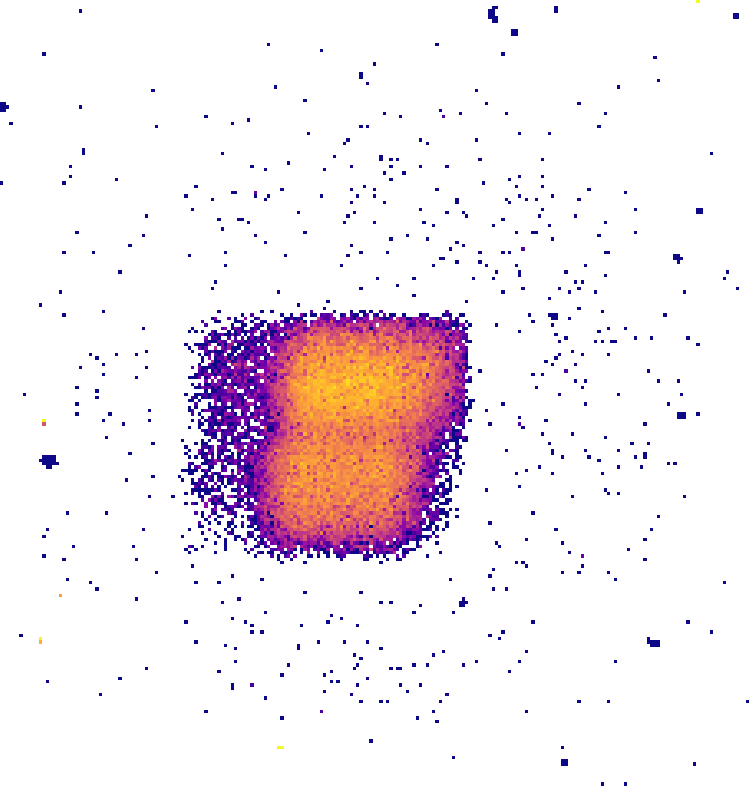
\includegraphics[interpolate=true,width=1.428000in,height=1.498000in]{th_180_450_600-img0.png}}%
\end{pgfscope}%
\begin{pgfscope}%
\pgfpathrectangle{\pgfqpoint{0.159098in}{0.074827in}}{\pgfqpoint{1.590982in}{1.508933in}}%
\pgfusepath{clip}%
\pgfsetbuttcap%
\pgfsetmiterjoin%
\pgfsetlinewidth{1.003750pt}%
\definecolor{currentstroke}{rgb}{0.000000,0.501961,0.000000}%
\pgfsetstrokecolor{currentstroke}%
\pgfsetdash{}{0pt}%
\pgfpathmoveto{\pgfqpoint{0.335140in}{0.659539in}}%
\pgfpathcurveto{\pgfqpoint{0.343477in}{0.659539in}}{\pgfqpoint{0.351474in}{0.662851in}}{\pgfqpoint{0.357369in}{0.668746in}}%
\pgfpathcurveto{\pgfqpoint{0.363264in}{0.674642in}}{\pgfqpoint{0.366577in}{0.682638in}}{\pgfqpoint{0.366577in}{0.690975in}}%
\pgfpathcurveto{\pgfqpoint{0.366577in}{0.699312in}}{\pgfqpoint{0.363264in}{0.707309in}}{\pgfqpoint{0.357369in}{0.713204in}}%
\pgfpathcurveto{\pgfqpoint{0.351474in}{0.719099in}}{\pgfqpoint{0.343477in}{0.722411in}}{\pgfqpoint{0.335140in}{0.722411in}}%
\pgfpathcurveto{\pgfqpoint{0.326803in}{0.722411in}}{\pgfqpoint{0.318807in}{0.719099in}}{\pgfqpoint{0.312912in}{0.713204in}}%
\pgfpathcurveto{\pgfqpoint{0.307017in}{0.707309in}}{\pgfqpoint{0.303704in}{0.699312in}}{\pgfqpoint{0.303704in}{0.690975in}}%
\pgfpathcurveto{\pgfqpoint{0.303704in}{0.682638in}}{\pgfqpoint{0.307017in}{0.674642in}}{\pgfqpoint{0.312912in}{0.668746in}}%
\pgfpathcurveto{\pgfqpoint{0.318807in}{0.662851in}}{\pgfqpoint{0.326803in}{0.659539in}}{\pgfqpoint{0.335140in}{0.659539in}}%
\pgfpathlineto{\pgfqpoint{0.335140in}{0.659539in}}%
\pgfpathclose%
\pgfusepath{stroke}%
\end{pgfscope}%
\begin{pgfscope}%
\pgfpathrectangle{\pgfqpoint{0.159098in}{0.074827in}}{\pgfqpoint{1.590982in}{1.508933in}}%
\pgfusepath{clip}%
\pgfsetbuttcap%
\pgfsetmiterjoin%
\pgfsetlinewidth{1.003750pt}%
\definecolor{currentstroke}{rgb}{0.000000,0.501961,0.000000}%
\pgfsetstrokecolor{currentstroke}%
\pgfsetdash{}{0pt}%
\pgfpathmoveto{\pgfqpoint{1.177628in}{1.508314in}}%
\pgfpathcurveto{\pgfqpoint{1.185965in}{1.508314in}}{\pgfqpoint{1.193962in}{1.511626in}}{\pgfqpoint{1.199857in}{1.517522in}}%
\pgfpathcurveto{\pgfqpoint{1.205752in}{1.523417in}}{\pgfqpoint{1.209064in}{1.531413in}}{\pgfqpoint{1.209064in}{1.539750in}}%
\pgfpathcurveto{\pgfqpoint{1.209064in}{1.548087in}}{\pgfqpoint{1.205752in}{1.556084in}}{\pgfqpoint{1.199857in}{1.561979in}}%
\pgfpathcurveto{\pgfqpoint{1.193962in}{1.567874in}}{\pgfqpoint{1.185965in}{1.571186in}}{\pgfqpoint{1.177628in}{1.571186in}}%
\pgfpathcurveto{\pgfqpoint{1.169291in}{1.571186in}}{\pgfqpoint{1.161295in}{1.567874in}}{\pgfqpoint{1.155400in}{1.561979in}}%
\pgfpathcurveto{\pgfqpoint{1.149504in}{1.556084in}}{\pgfqpoint{1.146192in}{1.548087in}}{\pgfqpoint{1.146192in}{1.539750in}}%
\pgfpathcurveto{\pgfqpoint{1.146192in}{1.531413in}}{\pgfqpoint{1.149504in}{1.523417in}}{\pgfqpoint{1.155400in}{1.517522in}}%
\pgfpathcurveto{\pgfqpoint{1.161295in}{1.511626in}}{\pgfqpoint{1.169291in}{1.508314in}}{\pgfqpoint{1.177628in}{1.508314in}}%
\pgfpathlineto{\pgfqpoint{1.177628in}{1.508314in}}%
\pgfpathclose%
\pgfusepath{stroke}%
\end{pgfscope}%
\begin{pgfscope}%
\pgfpathrectangle{\pgfqpoint{0.159098in}{0.074827in}}{\pgfqpoint{1.590982in}{1.508933in}}%
\pgfusepath{clip}%
\pgfsetbuttcap%
\pgfsetmiterjoin%
\pgfsetlinewidth{1.003750pt}%
\definecolor{currentstroke}{rgb}{0.000000,0.501961,0.000000}%
\pgfsetstrokecolor{currentstroke}%
\pgfsetdash{}{0pt}%
\pgfpathmoveto{\pgfqpoint{1.529713in}{1.043060in}}%
\pgfpathcurveto{\pgfqpoint{1.538050in}{1.043060in}}{\pgfqpoint{1.546046in}{1.046372in}}{\pgfqpoint{1.551941in}{1.052267in}}%
\pgfpathcurveto{\pgfqpoint{1.557836in}{1.058162in}}{\pgfqpoint{1.561149in}{1.066159in}}{\pgfqpoint{1.561149in}{1.074496in}}%
\pgfpathcurveto{\pgfqpoint{1.561149in}{1.082833in}}{\pgfqpoint{1.557836in}{1.090829in}}{\pgfqpoint{1.551941in}{1.096724in}}%
\pgfpathcurveto{\pgfqpoint{1.546046in}{1.102620in}}{\pgfqpoint{1.538050in}{1.105932in}}{\pgfqpoint{1.529713in}{1.105932in}}%
\pgfpathcurveto{\pgfqpoint{1.521376in}{1.105932in}}{\pgfqpoint{1.513379in}{1.102620in}}{\pgfqpoint{1.507484in}{1.096724in}}%
\pgfpathcurveto{\pgfqpoint{1.501589in}{1.090829in}}{\pgfqpoint{1.498277in}{1.082833in}}{\pgfqpoint{1.498277in}{1.074496in}}%
\pgfpathcurveto{\pgfqpoint{1.498277in}{1.066159in}}{\pgfqpoint{1.501589in}{1.058162in}}{\pgfqpoint{1.507484in}{1.052267in}}%
\pgfpathcurveto{\pgfqpoint{1.513379in}{1.046372in}}{\pgfqpoint{1.521376in}{1.043060in}}{\pgfqpoint{1.529713in}{1.043060in}}%
\pgfpathlineto{\pgfqpoint{1.529713in}{1.043060in}}%
\pgfpathclose%
\pgfusepath{stroke}%
\end{pgfscope}%
\begin{pgfscope}%
\pgfpathrectangle{\pgfqpoint{0.159098in}{0.074827in}}{\pgfqpoint{1.590982in}{1.508933in}}%
\pgfusepath{clip}%
\pgfsetbuttcap%
\pgfsetmiterjoin%
\pgfsetlinewidth{1.003750pt}%
\definecolor{currentstroke}{rgb}{0.000000,0.501961,0.000000}%
\pgfsetstrokecolor{currentstroke}%
\pgfsetdash{}{0pt}%
\pgfpathmoveto{\pgfqpoint{1.309660in}{0.087402in}}%
\pgfpathcurveto{\pgfqpoint{1.317997in}{0.087402in}}{\pgfqpoint{1.325993in}{0.090714in}}{\pgfqpoint{1.331889in}{0.096609in}}%
\pgfpathcurveto{\pgfqpoint{1.337784in}{0.102504in}}{\pgfqpoint{1.341096in}{0.110501in}}{\pgfqpoint{1.341096in}{0.118838in}}%
\pgfpathcurveto{\pgfqpoint{1.341096in}{0.127175in}}{\pgfqpoint{1.337784in}{0.135171in}}{\pgfqpoint{1.331889in}{0.141067in}}%
\pgfpathcurveto{\pgfqpoint{1.325993in}{0.146962in}}{\pgfqpoint{1.317997in}{0.150274in}}{\pgfqpoint{1.309660in}{0.150274in}}%
\pgfpathcurveto{\pgfqpoint{1.301323in}{0.150274in}}{\pgfqpoint{1.293326in}{0.146962in}}{\pgfqpoint{1.287431in}{0.141067in}}%
\pgfpathcurveto{\pgfqpoint{1.281536in}{0.135171in}}{\pgfqpoint{1.278224in}{0.127175in}}{\pgfqpoint{1.278224in}{0.118838in}}%
\pgfpathcurveto{\pgfqpoint{1.278224in}{0.110501in}}{\pgfqpoint{1.281536in}{0.102504in}}{\pgfqpoint{1.287431in}{0.096609in}}%
\pgfpathcurveto{\pgfqpoint{1.293326in}{0.090714in}}{\pgfqpoint{1.301323in}{0.087402in}}{\pgfqpoint{1.309660in}{0.087402in}}%
\pgfpathlineto{\pgfqpoint{1.309660in}{0.087402in}}%
\pgfpathclose%
\pgfusepath{stroke}%
\end{pgfscope}%
\begin{pgfscope}%
\pgfpathrectangle{\pgfqpoint{0.159098in}{0.074827in}}{\pgfqpoint{1.590982in}{1.508933in}}%
\pgfusepath{clip}%
\pgfsetbuttcap%
\pgfsetmiterjoin%
\pgfsetlinewidth{1.003750pt}%
\definecolor{currentstroke}{rgb}{0.000000,0.501961,0.000000}%
\pgfsetstrokecolor{currentstroke}%
\pgfsetdash{}{0pt}%
\pgfpathmoveto{\pgfqpoint{1.297085in}{0.936177in}}%
\pgfpathcurveto{\pgfqpoint{1.305422in}{0.936177in}}{\pgfqpoint{1.313419in}{0.939489in}}{\pgfqpoint{1.319314in}{0.945384in}}%
\pgfpathcurveto{\pgfqpoint{1.325209in}{0.951279in}}{\pgfqpoint{1.328522in}{0.959276in}}{\pgfqpoint{1.328522in}{0.967613in}}%
\pgfpathcurveto{\pgfqpoint{1.328522in}{0.975950in}}{\pgfqpoint{1.325209in}{0.983947in}}{\pgfqpoint{1.319314in}{0.989842in}}%
\pgfpathcurveto{\pgfqpoint{1.313419in}{0.995737in}}{\pgfqpoint{1.305422in}{0.999049in}}{\pgfqpoint{1.297085in}{0.999049in}}%
\pgfpathcurveto{\pgfqpoint{1.288748in}{0.999049in}}{\pgfqpoint{1.280752in}{0.995737in}}{\pgfqpoint{1.274857in}{0.989842in}}%
\pgfpathcurveto{\pgfqpoint{1.268962in}{0.983947in}}{\pgfqpoint{1.265649in}{0.975950in}}{\pgfqpoint{1.265649in}{0.967613in}}%
\pgfpathcurveto{\pgfqpoint{1.265649in}{0.959276in}}{\pgfqpoint{1.268962in}{0.951279in}}{\pgfqpoint{1.274857in}{0.945384in}}%
\pgfpathcurveto{\pgfqpoint{1.280752in}{0.939489in}}{\pgfqpoint{1.288748in}{0.936177in}}{\pgfqpoint{1.297085in}{0.936177in}}%
\pgfpathlineto{\pgfqpoint{1.297085in}{0.936177in}}%
\pgfpathclose%
\pgfusepath{stroke}%
\end{pgfscope}%
\begin{pgfscope}%
\pgfpathrectangle{\pgfqpoint{0.159098in}{0.074827in}}{\pgfqpoint{1.590982in}{1.508933in}}%
\pgfusepath{clip}%
\pgfsetbuttcap%
\pgfsetmiterjoin%
\pgfsetlinewidth{1.003750pt}%
\definecolor{currentstroke}{rgb}{0.000000,0.501961,0.000000}%
\pgfsetstrokecolor{currentstroke}%
\pgfsetdash{}{0pt}%
\pgfpathmoveto{\pgfqpoint{1.542287in}{0.753847in}}%
\pgfpathcurveto{\pgfqpoint{1.550624in}{0.753847in}}{\pgfqpoint{1.558621in}{0.757160in}}{\pgfqpoint{1.564516in}{0.763055in}}%
\pgfpathcurveto{\pgfqpoint{1.570411in}{0.768950in}}{\pgfqpoint{1.573723in}{0.776947in}}{\pgfqpoint{1.573723in}{0.785284in}}%
\pgfpathcurveto{\pgfqpoint{1.573723in}{0.793620in}}{\pgfqpoint{1.570411in}{0.801617in}}{\pgfqpoint{1.564516in}{0.807512in}}%
\pgfpathcurveto{\pgfqpoint{1.558621in}{0.813407in}}{\pgfqpoint{1.550624in}{0.816720in}}{\pgfqpoint{1.542287in}{0.816720in}}%
\pgfpathcurveto{\pgfqpoint{1.533950in}{0.816720in}}{\pgfqpoint{1.525954in}{0.813407in}}{\pgfqpoint{1.520058in}{0.807512in}}%
\pgfpathcurveto{\pgfqpoint{1.514163in}{0.801617in}}{\pgfqpoint{1.510851in}{0.793620in}}{\pgfqpoint{1.510851in}{0.785284in}}%
\pgfpathcurveto{\pgfqpoint{1.510851in}{0.776947in}}{\pgfqpoint{1.514163in}{0.768950in}}{\pgfqpoint{1.520058in}{0.763055in}}%
\pgfpathcurveto{\pgfqpoint{1.525954in}{0.757160in}}{\pgfqpoint{1.533950in}{0.753847in}}{\pgfqpoint{1.542287in}{0.753847in}}%
\pgfpathlineto{\pgfqpoint{1.542287in}{0.753847in}}%
\pgfpathclose%
\pgfusepath{stroke}%
\end{pgfscope}%
\begin{pgfscope}%
\pgfpathrectangle{\pgfqpoint{0.159098in}{0.074827in}}{\pgfqpoint{1.590982in}{1.508933in}}%
\pgfusepath{clip}%
\pgfsetbuttcap%
\pgfsetmiterjoin%
\pgfsetlinewidth{1.003750pt}%
\definecolor{currentstroke}{rgb}{0.000000,0.501961,0.000000}%
\pgfsetstrokecolor{currentstroke}%
\pgfsetdash{}{0pt}%
\pgfpathmoveto{\pgfqpoint{1.479415in}{0.313742in}}%
\pgfpathcurveto{\pgfqpoint{1.487752in}{0.313742in}}{\pgfqpoint{1.495748in}{0.317054in}}{\pgfqpoint{1.501644in}{0.322949in}}%
\pgfpathcurveto{\pgfqpoint{1.507539in}{0.328844in}}{\pgfqpoint{1.510851in}{0.336841in}}{\pgfqpoint{1.510851in}{0.345178in}}%
\pgfpathcurveto{\pgfqpoint{1.510851in}{0.353515in}}{\pgfqpoint{1.507539in}{0.361512in}}{\pgfqpoint{1.501644in}{0.367407in}}%
\pgfpathcurveto{\pgfqpoint{1.495748in}{0.373302in}}{\pgfqpoint{1.487752in}{0.376614in}}{\pgfqpoint{1.479415in}{0.376614in}}%
\pgfpathcurveto{\pgfqpoint{1.471078in}{0.376614in}}{\pgfqpoint{1.463081in}{0.373302in}}{\pgfqpoint{1.457186in}{0.367407in}}%
\pgfpathcurveto{\pgfqpoint{1.451291in}{0.361512in}}{\pgfqpoint{1.447979in}{0.353515in}}{\pgfqpoint{1.447979in}{0.345178in}}%
\pgfpathcurveto{\pgfqpoint{1.447979in}{0.336841in}}{\pgfqpoint{1.451291in}{0.328844in}}{\pgfqpoint{1.457186in}{0.322949in}}%
\pgfpathcurveto{\pgfqpoint{1.463081in}{0.317054in}}{\pgfqpoint{1.471078in}{0.313742in}}{\pgfqpoint{1.479415in}{0.313742in}}%
\pgfpathlineto{\pgfqpoint{1.479415in}{0.313742in}}%
\pgfpathclose%
\pgfusepath{stroke}%
\end{pgfscope}%
\begin{pgfscope}%
\pgfpathrectangle{\pgfqpoint{0.159098in}{0.074827in}}{\pgfqpoint{1.590982in}{1.508933in}}%
\pgfusepath{clip}%
\pgfsetbuttcap%
\pgfsetmiterjoin%
\pgfsetlinewidth{1.003750pt}%
\definecolor{currentstroke}{rgb}{0.000000,0.501961,0.000000}%
\pgfsetstrokecolor{currentstroke}%
\pgfsetdash{}{0pt}%
\pgfpathmoveto{\pgfqpoint{0.240832in}{1.338559in}}%
\pgfpathcurveto{\pgfqpoint{0.249169in}{1.338559in}}{\pgfqpoint{0.257166in}{1.341871in}}{\pgfqpoint{0.263061in}{1.347767in}}%
\pgfpathcurveto{\pgfqpoint{0.268956in}{1.353662in}}{\pgfqpoint{0.272268in}{1.361658in}}{\pgfqpoint{0.272268in}{1.369995in}}%
\pgfpathcurveto{\pgfqpoint{0.272268in}{1.378332in}}{\pgfqpoint{0.268956in}{1.386329in}}{\pgfqpoint{0.263061in}{1.392224in}}%
\pgfpathcurveto{\pgfqpoint{0.257166in}{1.398119in}}{\pgfqpoint{0.249169in}{1.401431in}}{\pgfqpoint{0.240832in}{1.401431in}}%
\pgfpathcurveto{\pgfqpoint{0.232495in}{1.401431in}}{\pgfqpoint{0.224498in}{1.398119in}}{\pgfqpoint{0.218603in}{1.392224in}}%
\pgfpathcurveto{\pgfqpoint{0.212708in}{1.386329in}}{\pgfqpoint{0.209396in}{1.378332in}}{\pgfqpoint{0.209396in}{1.369995in}}%
\pgfpathcurveto{\pgfqpoint{0.209396in}{1.361658in}}{\pgfqpoint{0.212708in}{1.353662in}}{\pgfqpoint{0.218603in}{1.347767in}}%
\pgfpathcurveto{\pgfqpoint{0.224498in}{1.341871in}}{\pgfqpoint{0.232495in}{1.338559in}}{\pgfqpoint{0.240832in}{1.338559in}}%
\pgfpathlineto{\pgfqpoint{0.240832in}{1.338559in}}%
\pgfpathclose%
\pgfusepath{stroke}%
\end{pgfscope}%
\begin{pgfscope}%
\pgfpathrectangle{\pgfqpoint{0.159098in}{0.074827in}}{\pgfqpoint{1.590982in}{1.508933in}}%
\pgfusepath{clip}%
\pgfsetbuttcap%
\pgfsetmiterjoin%
\pgfsetlinewidth{1.003750pt}%
\definecolor{currentstroke}{rgb}{0.000000,0.501961,0.000000}%
\pgfsetstrokecolor{currentstroke}%
\pgfsetdash{}{0pt}%
\pgfpathmoveto{\pgfqpoint{1.114756in}{0.389188in}}%
\pgfpathcurveto{\pgfqpoint{1.123093in}{0.389188in}}{\pgfqpoint{1.131090in}{0.392501in}}{\pgfqpoint{1.136985in}{0.398396in}}%
\pgfpathcurveto{\pgfqpoint{1.142880in}{0.404291in}}{\pgfqpoint{1.146192in}{0.412288in}}{\pgfqpoint{1.146192in}{0.420625in}}%
\pgfpathcurveto{\pgfqpoint{1.146192in}{0.428962in}}{\pgfqpoint{1.142880in}{0.436958in}}{\pgfqpoint{1.136985in}{0.442853in}}%
\pgfpathcurveto{\pgfqpoint{1.131090in}{0.448748in}}{\pgfqpoint{1.123093in}{0.452061in}}{\pgfqpoint{1.114756in}{0.452061in}}%
\pgfpathcurveto{\pgfqpoint{1.106419in}{0.452061in}}{\pgfqpoint{1.098422in}{0.448748in}}{\pgfqpoint{1.092527in}{0.442853in}}%
\pgfpathcurveto{\pgfqpoint{1.086632in}{0.436958in}}{\pgfqpoint{1.083320in}{0.428962in}}{\pgfqpoint{1.083320in}{0.420625in}}%
\pgfpathcurveto{\pgfqpoint{1.083320in}{0.412288in}}{\pgfqpoint{1.086632in}{0.404291in}}{\pgfqpoint{1.092527in}{0.398396in}}%
\pgfpathcurveto{\pgfqpoint{1.098422in}{0.392501in}}{\pgfqpoint{1.106419in}{0.389188in}}{\pgfqpoint{1.114756in}{0.389188in}}%
\pgfpathlineto{\pgfqpoint{1.114756in}{0.389188in}}%
\pgfpathclose%
\pgfusepath{stroke}%
\end{pgfscope}%
\begin{pgfscope}%
\pgfpathrectangle{\pgfqpoint{0.159098in}{0.074827in}}{\pgfqpoint{1.590982in}{1.508933in}}%
\pgfusepath{clip}%
\pgfsetbuttcap%
\pgfsetmiterjoin%
\pgfsetlinewidth{1.003750pt}%
\definecolor{currentstroke}{rgb}{0.000000,0.501961,0.000000}%
\pgfsetstrokecolor{currentstroke}%
\pgfsetdash{}{0pt}%
\pgfpathmoveto{\pgfqpoint{1.642883in}{1.502027in}}%
\pgfpathcurveto{\pgfqpoint{1.651220in}{1.502027in}}{\pgfqpoint{1.659216in}{1.505339in}}{\pgfqpoint{1.665111in}{1.511234in}}%
\pgfpathcurveto{\pgfqpoint{1.671006in}{1.517129in}}{\pgfqpoint{1.674319in}{1.525126in}}{\pgfqpoint{1.674319in}{1.533463in}}%
\pgfpathcurveto{\pgfqpoint{1.674319in}{1.541800in}}{\pgfqpoint{1.671006in}{1.549797in}}{\pgfqpoint{1.665111in}{1.555692in}}%
\pgfpathcurveto{\pgfqpoint{1.659216in}{1.561587in}}{\pgfqpoint{1.651220in}{1.564899in}}{\pgfqpoint{1.642883in}{1.564899in}}%
\pgfpathcurveto{\pgfqpoint{1.634546in}{1.564899in}}{\pgfqpoint{1.626549in}{1.561587in}}{\pgfqpoint{1.620654in}{1.555692in}}%
\pgfpathcurveto{\pgfqpoint{1.614759in}{1.549797in}}{\pgfqpoint{1.611447in}{1.541800in}}{\pgfqpoint{1.611447in}{1.533463in}}%
\pgfpathcurveto{\pgfqpoint{1.611447in}{1.525126in}}{\pgfqpoint{1.614759in}{1.517129in}}{\pgfqpoint{1.620654in}{1.511234in}}%
\pgfpathcurveto{\pgfqpoint{1.626549in}{1.505339in}}{\pgfqpoint{1.634546in}{1.502027in}}{\pgfqpoint{1.642883in}{1.502027in}}%
\pgfpathlineto{\pgfqpoint{1.642883in}{1.502027in}}%
\pgfpathclose%
\pgfusepath{stroke}%
\end{pgfscope}%
\begin{pgfscope}%
\pgfpathrectangle{\pgfqpoint{0.159098in}{0.074827in}}{\pgfqpoint{1.590982in}{1.508933in}}%
\pgfusepath{clip}%
\pgfsetbuttcap%
\pgfsetmiterjoin%
\pgfsetlinewidth{1.003750pt}%
\definecolor{currentstroke}{rgb}{0.000000,0.501961,0.000000}%
\pgfsetstrokecolor{currentstroke}%
\pgfsetdash{}{0pt}%
\pgfpathmoveto{\pgfqpoint{1.573723in}{1.137368in}}%
\pgfpathcurveto{\pgfqpoint{1.582060in}{1.137368in}}{\pgfqpoint{1.590057in}{1.140680in}}{\pgfqpoint{1.595952in}{1.146575in}}%
\pgfpathcurveto{\pgfqpoint{1.601847in}{1.152471in}}{\pgfqpoint{1.605159in}{1.160467in}}{\pgfqpoint{1.605159in}{1.168804in}}%
\pgfpathcurveto{\pgfqpoint{1.605159in}{1.177141in}}{\pgfqpoint{1.601847in}{1.185138in}}{\pgfqpoint{1.595952in}{1.191033in}}%
\pgfpathcurveto{\pgfqpoint{1.590057in}{1.196928in}}{\pgfqpoint{1.582060in}{1.200240in}}{\pgfqpoint{1.573723in}{1.200240in}}%
\pgfpathcurveto{\pgfqpoint{1.565386in}{1.200240in}}{\pgfqpoint{1.557390in}{1.196928in}}{\pgfqpoint{1.551495in}{1.191033in}}%
\pgfpathcurveto{\pgfqpoint{1.545599in}{1.185138in}}{\pgfqpoint{1.542287in}{1.177141in}}{\pgfqpoint{1.542287in}{1.168804in}}%
\pgfpathcurveto{\pgfqpoint{1.542287in}{1.160467in}}{\pgfqpoint{1.545599in}{1.152471in}}{\pgfqpoint{1.551495in}{1.146575in}}%
\pgfpathcurveto{\pgfqpoint{1.557390in}{1.140680in}}{\pgfqpoint{1.565386in}{1.137368in}}{\pgfqpoint{1.573723in}{1.137368in}}%
\pgfpathlineto{\pgfqpoint{1.573723in}{1.137368in}}%
\pgfpathclose%
\pgfusepath{stroke}%
\end{pgfscope}%
\begin{pgfscope}%
\pgfsetrectcap%
\pgfsetmiterjoin%
\pgfsetlinewidth{0.803000pt}%
\definecolor{currentstroke}{rgb}{0.000000,0.000000,0.000000}%
\pgfsetstrokecolor{currentstroke}%
\pgfsetdash{}{0pt}%
\pgfpathmoveto{\pgfqpoint{0.159098in}{0.074827in}}%
\pgfpathlineto{\pgfqpoint{0.159098in}{1.583761in}}%
\pgfusepath{stroke}%
\end{pgfscope}%
\begin{pgfscope}%
\pgfsetrectcap%
\pgfsetmiterjoin%
\pgfsetlinewidth{0.803000pt}%
\definecolor{currentstroke}{rgb}{0.000000,0.000000,0.000000}%
\pgfsetstrokecolor{currentstroke}%
\pgfsetdash{}{0pt}%
\pgfpathmoveto{\pgfqpoint{1.750080in}{0.074827in}}%
\pgfpathlineto{\pgfqpoint{1.750080in}{1.583761in}}%
\pgfusepath{stroke}%
\end{pgfscope}%
\begin{pgfscope}%
\pgfsetrectcap%
\pgfsetmiterjoin%
\pgfsetlinewidth{0.803000pt}%
\definecolor{currentstroke}{rgb}{0.000000,0.000000,0.000000}%
\pgfsetstrokecolor{currentstroke}%
\pgfsetdash{}{0pt}%
\pgfpathmoveto{\pgfqpoint{0.159098in}{0.074827in}}%
\pgfpathlineto{\pgfqpoint{1.750080in}{0.074827in}}%
\pgfusepath{stroke}%
\end{pgfscope}%
\begin{pgfscope}%
\pgfsetrectcap%
\pgfsetmiterjoin%
\pgfsetlinewidth{0.803000pt}%
\definecolor{currentstroke}{rgb}{0.000000,0.000000,0.000000}%
\pgfsetstrokecolor{currentstroke}%
\pgfsetdash{}{0pt}%
\pgfpathmoveto{\pgfqpoint{0.159098in}{1.583761in}}%
\pgfpathlineto{\pgfqpoint{1.750080in}{1.583761in}}%
\pgfusepath{stroke}%
\end{pgfscope}%
\begin{pgfscope}%
\definecolor{textcolor}{rgb}{0.000000,0.000000,0.000000}%
\pgfsetstrokecolor{textcolor}%
\pgfsetfillcolor{textcolor}%
\pgftext[x=-0.000000in,y=1.734654in,left,base]{\color{textcolor}\rmfamily\fontsize{10.000000}{12.000000}\selectfont (a)}%
\end{pgfscope}%
\begin{pgfscope}%
\pgfsetbuttcap%
\pgfsetmiterjoin%
\definecolor{currentfill}{rgb}{1.000000,1.000000,1.000000}%
\pgfsetfillcolor{currentfill}%
\pgfsetlinewidth{0.000000pt}%
\definecolor{currentstroke}{rgb}{0.000000,0.000000,0.000000}%
\pgfsetstrokecolor{currentstroke}%
\pgfsetstrokeopacity{0.000000}%
\pgfsetdash{}{0pt}%
\pgfpathmoveto{\pgfqpoint{1.950080in}{0.074827in}}%
\pgfpathlineto{\pgfqpoint{3.541061in}{0.074827in}}%
\pgfpathlineto{\pgfqpoint{3.541061in}{1.583761in}}%
\pgfpathlineto{\pgfqpoint{1.950080in}{1.583761in}}%
\pgfpathlineto{\pgfqpoint{1.950080in}{0.074827in}}%
\pgfpathclose%
\pgfusepath{fill}%
\end{pgfscope}%
\begin{pgfscope}%
\pgfsys@transformshift{2.032000in}{0.112795in}%
\pgftext[left,bottom]{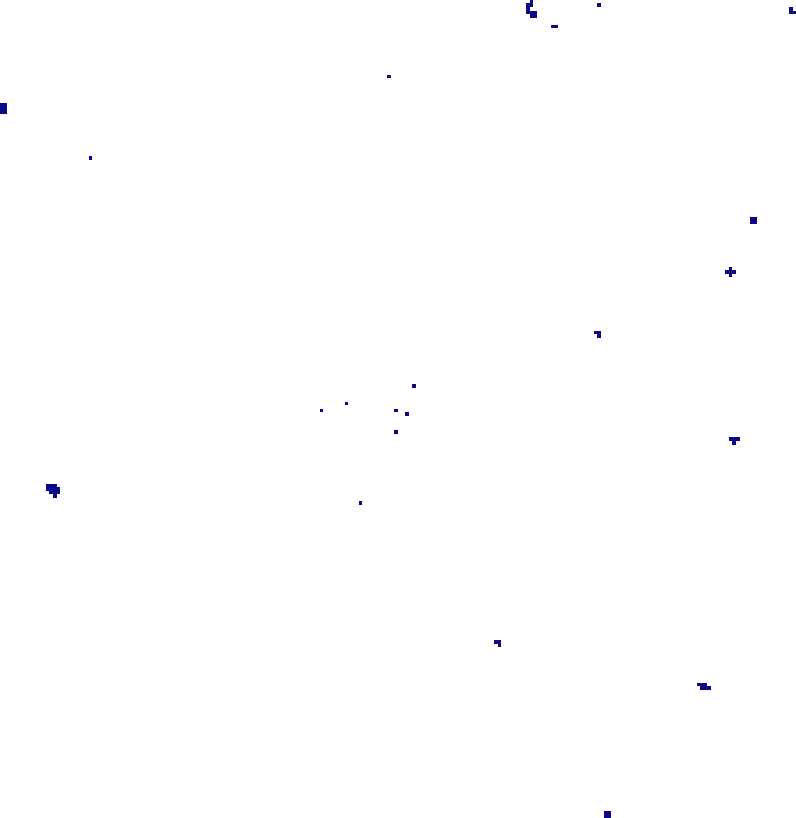
\includegraphics[interpolate=true,width=1.408000in,height=1.446000in]{th_180_450_600-img1.png}}%
\end{pgfscope}%
\begin{pgfscope}%
\pgfpathrectangle{\pgfqpoint{1.950080in}{0.074827in}}{\pgfqpoint{1.590982in}{1.508933in}}%
\pgfusepath{clip}%
\pgfsetbuttcap%
\pgfsetmiterjoin%
\pgfsetlinewidth{1.003750pt}%
\definecolor{currentstroke}{rgb}{0.000000,0.501961,0.000000}%
\pgfsetstrokecolor{currentstroke}%
\pgfsetdash{}{0pt}%
\pgfpathmoveto{\pgfqpoint{2.126122in}{0.659539in}}%
\pgfpathcurveto{\pgfqpoint{2.134459in}{0.659539in}}{\pgfqpoint{2.142456in}{0.662851in}}{\pgfqpoint{2.148351in}{0.668746in}}%
\pgfpathcurveto{\pgfqpoint{2.154246in}{0.674642in}}{\pgfqpoint{2.157558in}{0.682638in}}{\pgfqpoint{2.157558in}{0.690975in}}%
\pgfpathcurveto{\pgfqpoint{2.157558in}{0.699312in}}{\pgfqpoint{2.154246in}{0.707309in}}{\pgfqpoint{2.148351in}{0.713204in}}%
\pgfpathcurveto{\pgfqpoint{2.142456in}{0.719099in}}{\pgfqpoint{2.134459in}{0.722411in}}{\pgfqpoint{2.126122in}{0.722411in}}%
\pgfpathcurveto{\pgfqpoint{2.117785in}{0.722411in}}{\pgfqpoint{2.109788in}{0.719099in}}{\pgfqpoint{2.103893in}{0.713204in}}%
\pgfpathcurveto{\pgfqpoint{2.097998in}{0.707309in}}{\pgfqpoint{2.094686in}{0.699312in}}{\pgfqpoint{2.094686in}{0.690975in}}%
\pgfpathcurveto{\pgfqpoint{2.094686in}{0.682638in}}{\pgfqpoint{2.097998in}{0.674642in}}{\pgfqpoint{2.103893in}{0.668746in}}%
\pgfpathcurveto{\pgfqpoint{2.109788in}{0.662851in}}{\pgfqpoint{2.117785in}{0.659539in}}{\pgfqpoint{2.126122in}{0.659539in}}%
\pgfpathlineto{\pgfqpoint{2.126122in}{0.659539in}}%
\pgfpathclose%
\pgfusepath{stroke}%
\end{pgfscope}%
\begin{pgfscope}%
\pgfpathrectangle{\pgfqpoint{1.950080in}{0.074827in}}{\pgfqpoint{1.590982in}{1.508933in}}%
\pgfusepath{clip}%
\pgfsetbuttcap%
\pgfsetmiterjoin%
\pgfsetlinewidth{1.003750pt}%
\definecolor{currentstroke}{rgb}{0.000000,0.501961,0.000000}%
\pgfsetstrokecolor{currentstroke}%
\pgfsetdash{}{0pt}%
\pgfpathmoveto{\pgfqpoint{2.968610in}{1.508314in}}%
\pgfpathcurveto{\pgfqpoint{2.976947in}{1.508314in}}{\pgfqpoint{2.984943in}{1.511626in}}{\pgfqpoint{2.990839in}{1.517522in}}%
\pgfpathcurveto{\pgfqpoint{2.996734in}{1.523417in}}{\pgfqpoint{3.000046in}{1.531413in}}{\pgfqpoint{3.000046in}{1.539750in}}%
\pgfpathcurveto{\pgfqpoint{3.000046in}{1.548087in}}{\pgfqpoint{2.996734in}{1.556084in}}{\pgfqpoint{2.990839in}{1.561979in}}%
\pgfpathcurveto{\pgfqpoint{2.984943in}{1.567874in}}{\pgfqpoint{2.976947in}{1.571186in}}{\pgfqpoint{2.968610in}{1.571186in}}%
\pgfpathcurveto{\pgfqpoint{2.960273in}{1.571186in}}{\pgfqpoint{2.952276in}{1.567874in}}{\pgfqpoint{2.946381in}{1.561979in}}%
\pgfpathcurveto{\pgfqpoint{2.940486in}{1.556084in}}{\pgfqpoint{2.937174in}{1.548087in}}{\pgfqpoint{2.937174in}{1.539750in}}%
\pgfpathcurveto{\pgfqpoint{2.937174in}{1.531413in}}{\pgfqpoint{2.940486in}{1.523417in}}{\pgfqpoint{2.946381in}{1.517522in}}%
\pgfpathcurveto{\pgfqpoint{2.952276in}{1.511626in}}{\pgfqpoint{2.960273in}{1.508314in}}{\pgfqpoint{2.968610in}{1.508314in}}%
\pgfpathlineto{\pgfqpoint{2.968610in}{1.508314in}}%
\pgfpathclose%
\pgfusepath{stroke}%
\end{pgfscope}%
\begin{pgfscope}%
\pgfpathrectangle{\pgfqpoint{1.950080in}{0.074827in}}{\pgfqpoint{1.590982in}{1.508933in}}%
\pgfusepath{clip}%
\pgfsetbuttcap%
\pgfsetmiterjoin%
\pgfsetlinewidth{1.003750pt}%
\definecolor{currentstroke}{rgb}{0.000000,0.501961,0.000000}%
\pgfsetstrokecolor{currentstroke}%
\pgfsetdash{}{0pt}%
\pgfpathmoveto{\pgfqpoint{3.320694in}{1.043060in}}%
\pgfpathcurveto{\pgfqpoint{3.329031in}{1.043060in}}{\pgfqpoint{3.337028in}{1.046372in}}{\pgfqpoint{3.342923in}{1.052267in}}%
\pgfpathcurveto{\pgfqpoint{3.348818in}{1.058162in}}{\pgfqpoint{3.352130in}{1.066159in}}{\pgfqpoint{3.352130in}{1.074496in}}%
\pgfpathcurveto{\pgfqpoint{3.352130in}{1.082833in}}{\pgfqpoint{3.348818in}{1.090829in}}{\pgfqpoint{3.342923in}{1.096724in}}%
\pgfpathcurveto{\pgfqpoint{3.337028in}{1.102620in}}{\pgfqpoint{3.329031in}{1.105932in}}{\pgfqpoint{3.320694in}{1.105932in}}%
\pgfpathcurveto{\pgfqpoint{3.312357in}{1.105932in}}{\pgfqpoint{3.304361in}{1.102620in}}{\pgfqpoint{3.298466in}{1.096724in}}%
\pgfpathcurveto{\pgfqpoint{3.292571in}{1.090829in}}{\pgfqpoint{3.289258in}{1.082833in}}{\pgfqpoint{3.289258in}{1.074496in}}%
\pgfpathcurveto{\pgfqpoint{3.289258in}{1.066159in}}{\pgfqpoint{3.292571in}{1.058162in}}{\pgfqpoint{3.298466in}{1.052267in}}%
\pgfpathcurveto{\pgfqpoint{3.304361in}{1.046372in}}{\pgfqpoint{3.312357in}{1.043060in}}{\pgfqpoint{3.320694in}{1.043060in}}%
\pgfpathlineto{\pgfqpoint{3.320694in}{1.043060in}}%
\pgfpathclose%
\pgfusepath{stroke}%
\end{pgfscope}%
\begin{pgfscope}%
\pgfpathrectangle{\pgfqpoint{1.950080in}{0.074827in}}{\pgfqpoint{1.590982in}{1.508933in}}%
\pgfusepath{clip}%
\pgfsetbuttcap%
\pgfsetmiterjoin%
\pgfsetlinewidth{1.003750pt}%
\definecolor{currentstroke}{rgb}{0.000000,0.501961,0.000000}%
\pgfsetstrokecolor{currentstroke}%
\pgfsetdash{}{0pt}%
\pgfpathmoveto{\pgfqpoint{3.100642in}{0.087402in}}%
\pgfpathcurveto{\pgfqpoint{3.108979in}{0.087402in}}{\pgfqpoint{3.116975in}{0.090714in}}{\pgfqpoint{3.122870in}{0.096609in}}%
\pgfpathcurveto{\pgfqpoint{3.128765in}{0.102504in}}{\pgfqpoint{3.132078in}{0.110501in}}{\pgfqpoint{3.132078in}{0.118838in}}%
\pgfpathcurveto{\pgfqpoint{3.132078in}{0.127175in}}{\pgfqpoint{3.128765in}{0.135171in}}{\pgfqpoint{3.122870in}{0.141067in}}%
\pgfpathcurveto{\pgfqpoint{3.116975in}{0.146962in}}{\pgfqpoint{3.108979in}{0.150274in}}{\pgfqpoint{3.100642in}{0.150274in}}%
\pgfpathcurveto{\pgfqpoint{3.092305in}{0.150274in}}{\pgfqpoint{3.084308in}{0.146962in}}{\pgfqpoint{3.078413in}{0.141067in}}%
\pgfpathcurveto{\pgfqpoint{3.072518in}{0.135171in}}{\pgfqpoint{3.069205in}{0.127175in}}{\pgfqpoint{3.069205in}{0.118838in}}%
\pgfpathcurveto{\pgfqpoint{3.069205in}{0.110501in}}{\pgfqpoint{3.072518in}{0.102504in}}{\pgfqpoint{3.078413in}{0.096609in}}%
\pgfpathcurveto{\pgfqpoint{3.084308in}{0.090714in}}{\pgfqpoint{3.092305in}{0.087402in}}{\pgfqpoint{3.100642in}{0.087402in}}%
\pgfpathlineto{\pgfqpoint{3.100642in}{0.087402in}}%
\pgfpathclose%
\pgfusepath{stroke}%
\end{pgfscope}%
\begin{pgfscope}%
\pgfpathrectangle{\pgfqpoint{1.950080in}{0.074827in}}{\pgfqpoint{1.590982in}{1.508933in}}%
\pgfusepath{clip}%
\pgfsetbuttcap%
\pgfsetmiterjoin%
\pgfsetlinewidth{1.003750pt}%
\definecolor{currentstroke}{rgb}{0.000000,0.501961,0.000000}%
\pgfsetstrokecolor{currentstroke}%
\pgfsetdash{}{0pt}%
\pgfpathmoveto{\pgfqpoint{3.088067in}{0.936177in}}%
\pgfpathcurveto{\pgfqpoint{3.096404in}{0.936177in}}{\pgfqpoint{3.104401in}{0.939489in}}{\pgfqpoint{3.110296in}{0.945384in}}%
\pgfpathcurveto{\pgfqpoint{3.116191in}{0.951279in}}{\pgfqpoint{3.119503in}{0.959276in}}{\pgfqpoint{3.119503in}{0.967613in}}%
\pgfpathcurveto{\pgfqpoint{3.119503in}{0.975950in}}{\pgfqpoint{3.116191in}{0.983947in}}{\pgfqpoint{3.110296in}{0.989842in}}%
\pgfpathcurveto{\pgfqpoint{3.104401in}{0.995737in}}{\pgfqpoint{3.096404in}{0.999049in}}{\pgfqpoint{3.088067in}{0.999049in}}%
\pgfpathcurveto{\pgfqpoint{3.079730in}{0.999049in}}{\pgfqpoint{3.071734in}{0.995737in}}{\pgfqpoint{3.065838in}{0.989842in}}%
\pgfpathcurveto{\pgfqpoint{3.059943in}{0.983947in}}{\pgfqpoint{3.056631in}{0.975950in}}{\pgfqpoint{3.056631in}{0.967613in}}%
\pgfpathcurveto{\pgfqpoint{3.056631in}{0.959276in}}{\pgfqpoint{3.059943in}{0.951279in}}{\pgfqpoint{3.065838in}{0.945384in}}%
\pgfpathcurveto{\pgfqpoint{3.071734in}{0.939489in}}{\pgfqpoint{3.079730in}{0.936177in}}{\pgfqpoint{3.088067in}{0.936177in}}%
\pgfpathlineto{\pgfqpoint{3.088067in}{0.936177in}}%
\pgfpathclose%
\pgfusepath{stroke}%
\end{pgfscope}%
\begin{pgfscope}%
\pgfpathrectangle{\pgfqpoint{1.950080in}{0.074827in}}{\pgfqpoint{1.590982in}{1.508933in}}%
\pgfusepath{clip}%
\pgfsetbuttcap%
\pgfsetmiterjoin%
\pgfsetlinewidth{1.003750pt}%
\definecolor{currentstroke}{rgb}{0.000000,0.501961,0.000000}%
\pgfsetstrokecolor{currentstroke}%
\pgfsetdash{}{0pt}%
\pgfpathmoveto{\pgfqpoint{3.333269in}{0.753847in}}%
\pgfpathcurveto{\pgfqpoint{3.341606in}{0.753847in}}{\pgfqpoint{3.349602in}{0.757160in}}{\pgfqpoint{3.355497in}{0.763055in}}%
\pgfpathcurveto{\pgfqpoint{3.361393in}{0.768950in}}{\pgfqpoint{3.364705in}{0.776947in}}{\pgfqpoint{3.364705in}{0.785284in}}%
\pgfpathcurveto{\pgfqpoint{3.364705in}{0.793620in}}{\pgfqpoint{3.361393in}{0.801617in}}{\pgfqpoint{3.355497in}{0.807512in}}%
\pgfpathcurveto{\pgfqpoint{3.349602in}{0.813407in}}{\pgfqpoint{3.341606in}{0.816720in}}{\pgfqpoint{3.333269in}{0.816720in}}%
\pgfpathcurveto{\pgfqpoint{3.324932in}{0.816720in}}{\pgfqpoint{3.316935in}{0.813407in}}{\pgfqpoint{3.311040in}{0.807512in}}%
\pgfpathcurveto{\pgfqpoint{3.305145in}{0.801617in}}{\pgfqpoint{3.301833in}{0.793620in}}{\pgfqpoint{3.301833in}{0.785284in}}%
\pgfpathcurveto{\pgfqpoint{3.301833in}{0.776947in}}{\pgfqpoint{3.305145in}{0.768950in}}{\pgfqpoint{3.311040in}{0.763055in}}%
\pgfpathcurveto{\pgfqpoint{3.316935in}{0.757160in}}{\pgfqpoint{3.324932in}{0.753847in}}{\pgfqpoint{3.333269in}{0.753847in}}%
\pgfpathlineto{\pgfqpoint{3.333269in}{0.753847in}}%
\pgfpathclose%
\pgfusepath{stroke}%
\end{pgfscope}%
\begin{pgfscope}%
\pgfpathrectangle{\pgfqpoint{1.950080in}{0.074827in}}{\pgfqpoint{1.590982in}{1.508933in}}%
\pgfusepath{clip}%
\pgfsetbuttcap%
\pgfsetmiterjoin%
\pgfsetlinewidth{1.003750pt}%
\definecolor{currentstroke}{rgb}{0.000000,0.501961,0.000000}%
\pgfsetstrokecolor{currentstroke}%
\pgfsetdash{}{0pt}%
\pgfpathmoveto{\pgfqpoint{3.270397in}{0.313742in}}%
\pgfpathcurveto{\pgfqpoint{3.278734in}{0.313742in}}{\pgfqpoint{3.286730in}{0.317054in}}{\pgfqpoint{3.292625in}{0.322949in}}%
\pgfpathcurveto{\pgfqpoint{3.298520in}{0.328844in}}{\pgfqpoint{3.301833in}{0.336841in}}{\pgfqpoint{3.301833in}{0.345178in}}%
\pgfpathcurveto{\pgfqpoint{3.301833in}{0.353515in}}{\pgfqpoint{3.298520in}{0.361512in}}{\pgfqpoint{3.292625in}{0.367407in}}%
\pgfpathcurveto{\pgfqpoint{3.286730in}{0.373302in}}{\pgfqpoint{3.278734in}{0.376614in}}{\pgfqpoint{3.270397in}{0.376614in}}%
\pgfpathcurveto{\pgfqpoint{3.262060in}{0.376614in}}{\pgfqpoint{3.254063in}{0.373302in}}{\pgfqpoint{3.248168in}{0.367407in}}%
\pgfpathcurveto{\pgfqpoint{3.242273in}{0.361512in}}{\pgfqpoint{3.238960in}{0.353515in}}{\pgfqpoint{3.238960in}{0.345178in}}%
\pgfpathcurveto{\pgfqpoint{3.238960in}{0.336841in}}{\pgfqpoint{3.242273in}{0.328844in}}{\pgfqpoint{3.248168in}{0.322949in}}%
\pgfpathcurveto{\pgfqpoint{3.254063in}{0.317054in}}{\pgfqpoint{3.262060in}{0.313742in}}{\pgfqpoint{3.270397in}{0.313742in}}%
\pgfpathlineto{\pgfqpoint{3.270397in}{0.313742in}}%
\pgfpathclose%
\pgfusepath{stroke}%
\end{pgfscope}%
\begin{pgfscope}%
\pgfpathrectangle{\pgfqpoint{1.950080in}{0.074827in}}{\pgfqpoint{1.590982in}{1.508933in}}%
\pgfusepath{clip}%
\pgfsetbuttcap%
\pgfsetmiterjoin%
\pgfsetlinewidth{1.003750pt}%
\definecolor{currentstroke}{rgb}{0.000000,0.501961,0.000000}%
\pgfsetstrokecolor{currentstroke}%
\pgfsetdash{}{0pt}%
\pgfpathmoveto{\pgfqpoint{2.031814in}{1.338559in}}%
\pgfpathcurveto{\pgfqpoint{2.040151in}{1.338559in}}{\pgfqpoint{2.048147in}{1.341871in}}{\pgfqpoint{2.054042in}{1.347767in}}%
\pgfpathcurveto{\pgfqpoint{2.059938in}{1.353662in}}{\pgfqpoint{2.063250in}{1.361658in}}{\pgfqpoint{2.063250in}{1.369995in}}%
\pgfpathcurveto{\pgfqpoint{2.063250in}{1.378332in}}{\pgfqpoint{2.059938in}{1.386329in}}{\pgfqpoint{2.054042in}{1.392224in}}%
\pgfpathcurveto{\pgfqpoint{2.048147in}{1.398119in}}{\pgfqpoint{2.040151in}{1.401431in}}{\pgfqpoint{2.031814in}{1.401431in}}%
\pgfpathcurveto{\pgfqpoint{2.023477in}{1.401431in}}{\pgfqpoint{2.015480in}{1.398119in}}{\pgfqpoint{2.009585in}{1.392224in}}%
\pgfpathcurveto{\pgfqpoint{2.003690in}{1.386329in}}{\pgfqpoint{2.000378in}{1.378332in}}{\pgfqpoint{2.000378in}{1.369995in}}%
\pgfpathcurveto{\pgfqpoint{2.000378in}{1.361658in}}{\pgfqpoint{2.003690in}{1.353662in}}{\pgfqpoint{2.009585in}{1.347767in}}%
\pgfpathcurveto{\pgfqpoint{2.015480in}{1.341871in}}{\pgfqpoint{2.023477in}{1.338559in}}{\pgfqpoint{2.031814in}{1.338559in}}%
\pgfpathlineto{\pgfqpoint{2.031814in}{1.338559in}}%
\pgfpathclose%
\pgfusepath{stroke}%
\end{pgfscope}%
\begin{pgfscope}%
\pgfpathrectangle{\pgfqpoint{1.950080in}{0.074827in}}{\pgfqpoint{1.590982in}{1.508933in}}%
\pgfusepath{clip}%
\pgfsetbuttcap%
\pgfsetmiterjoin%
\pgfsetlinewidth{1.003750pt}%
\definecolor{currentstroke}{rgb}{0.000000,0.501961,0.000000}%
\pgfsetstrokecolor{currentstroke}%
\pgfsetdash{}{0pt}%
\pgfpathmoveto{\pgfqpoint{2.905738in}{0.389188in}}%
\pgfpathcurveto{\pgfqpoint{2.914075in}{0.389188in}}{\pgfqpoint{2.922071in}{0.392501in}}{\pgfqpoint{2.927966in}{0.398396in}}%
\pgfpathcurveto{\pgfqpoint{2.933861in}{0.404291in}}{\pgfqpoint{2.937174in}{0.412288in}}{\pgfqpoint{2.937174in}{0.420625in}}%
\pgfpathcurveto{\pgfqpoint{2.937174in}{0.428962in}}{\pgfqpoint{2.933861in}{0.436958in}}{\pgfqpoint{2.927966in}{0.442853in}}%
\pgfpathcurveto{\pgfqpoint{2.922071in}{0.448748in}}{\pgfqpoint{2.914075in}{0.452061in}}{\pgfqpoint{2.905738in}{0.452061in}}%
\pgfpathcurveto{\pgfqpoint{2.897401in}{0.452061in}}{\pgfqpoint{2.889404in}{0.448748in}}{\pgfqpoint{2.883509in}{0.442853in}}%
\pgfpathcurveto{\pgfqpoint{2.877614in}{0.436958in}}{\pgfqpoint{2.874302in}{0.428962in}}{\pgfqpoint{2.874302in}{0.420625in}}%
\pgfpathcurveto{\pgfqpoint{2.874302in}{0.412288in}}{\pgfqpoint{2.877614in}{0.404291in}}{\pgfqpoint{2.883509in}{0.398396in}}%
\pgfpathcurveto{\pgfqpoint{2.889404in}{0.392501in}}{\pgfqpoint{2.897401in}{0.389188in}}{\pgfqpoint{2.905738in}{0.389188in}}%
\pgfpathlineto{\pgfqpoint{2.905738in}{0.389188in}}%
\pgfpathclose%
\pgfusepath{stroke}%
\end{pgfscope}%
\begin{pgfscope}%
\pgfpathrectangle{\pgfqpoint{1.950080in}{0.074827in}}{\pgfqpoint{1.590982in}{1.508933in}}%
\pgfusepath{clip}%
\pgfsetbuttcap%
\pgfsetmiterjoin%
\pgfsetlinewidth{1.003750pt}%
\definecolor{currentstroke}{rgb}{0.000000,0.501961,0.000000}%
\pgfsetstrokecolor{currentstroke}%
\pgfsetdash{}{0pt}%
\pgfpathmoveto{\pgfqpoint{3.433864in}{1.502027in}}%
\pgfpathcurveto{\pgfqpoint{3.442201in}{1.502027in}}{\pgfqpoint{3.450198in}{1.505339in}}{\pgfqpoint{3.456093in}{1.511234in}}%
\pgfpathcurveto{\pgfqpoint{3.461988in}{1.517129in}}{\pgfqpoint{3.465300in}{1.525126in}}{\pgfqpoint{3.465300in}{1.533463in}}%
\pgfpathcurveto{\pgfqpoint{3.465300in}{1.541800in}}{\pgfqpoint{3.461988in}{1.549797in}}{\pgfqpoint{3.456093in}{1.555692in}}%
\pgfpathcurveto{\pgfqpoint{3.450198in}{1.561587in}}{\pgfqpoint{3.442201in}{1.564899in}}{\pgfqpoint{3.433864in}{1.564899in}}%
\pgfpathcurveto{\pgfqpoint{3.425527in}{1.564899in}}{\pgfqpoint{3.417531in}{1.561587in}}{\pgfqpoint{3.411636in}{1.555692in}}%
\pgfpathcurveto{\pgfqpoint{3.405741in}{1.549797in}}{\pgfqpoint{3.402428in}{1.541800in}}{\pgfqpoint{3.402428in}{1.533463in}}%
\pgfpathcurveto{\pgfqpoint{3.402428in}{1.525126in}}{\pgfqpoint{3.405741in}{1.517129in}}{\pgfqpoint{3.411636in}{1.511234in}}%
\pgfpathcurveto{\pgfqpoint{3.417531in}{1.505339in}}{\pgfqpoint{3.425527in}{1.502027in}}{\pgfqpoint{3.433864in}{1.502027in}}%
\pgfpathlineto{\pgfqpoint{3.433864in}{1.502027in}}%
\pgfpathclose%
\pgfusepath{stroke}%
\end{pgfscope}%
\begin{pgfscope}%
\pgfpathrectangle{\pgfqpoint{1.950080in}{0.074827in}}{\pgfqpoint{1.590982in}{1.508933in}}%
\pgfusepath{clip}%
\pgfsetbuttcap%
\pgfsetmiterjoin%
\pgfsetlinewidth{1.003750pt}%
\definecolor{currentstroke}{rgb}{0.000000,0.501961,0.000000}%
\pgfsetstrokecolor{currentstroke}%
\pgfsetdash{}{0pt}%
\pgfpathmoveto{\pgfqpoint{3.364705in}{1.137368in}}%
\pgfpathcurveto{\pgfqpoint{3.373042in}{1.137368in}}{\pgfqpoint{3.381038in}{1.140680in}}{\pgfqpoint{3.386934in}{1.146575in}}%
\pgfpathcurveto{\pgfqpoint{3.392829in}{1.152471in}}{\pgfqpoint{3.396141in}{1.160467in}}{\pgfqpoint{3.396141in}{1.168804in}}%
\pgfpathcurveto{\pgfqpoint{3.396141in}{1.177141in}}{\pgfqpoint{3.392829in}{1.185138in}}{\pgfqpoint{3.386934in}{1.191033in}}%
\pgfpathcurveto{\pgfqpoint{3.381038in}{1.196928in}}{\pgfqpoint{3.373042in}{1.200240in}}{\pgfqpoint{3.364705in}{1.200240in}}%
\pgfpathcurveto{\pgfqpoint{3.356368in}{1.200240in}}{\pgfqpoint{3.348371in}{1.196928in}}{\pgfqpoint{3.342476in}{1.191033in}}%
\pgfpathcurveto{\pgfqpoint{3.336581in}{1.185138in}}{\pgfqpoint{3.333269in}{1.177141in}}{\pgfqpoint{3.333269in}{1.168804in}}%
\pgfpathcurveto{\pgfqpoint{3.333269in}{1.160467in}}{\pgfqpoint{3.336581in}{1.152471in}}{\pgfqpoint{3.342476in}{1.146575in}}%
\pgfpathcurveto{\pgfqpoint{3.348371in}{1.140680in}}{\pgfqpoint{3.356368in}{1.137368in}}{\pgfqpoint{3.364705in}{1.137368in}}%
\pgfpathlineto{\pgfqpoint{3.364705in}{1.137368in}}%
\pgfpathclose%
\pgfusepath{stroke}%
\end{pgfscope}%
\begin{pgfscope}%
\pgfsetrectcap%
\pgfsetmiterjoin%
\pgfsetlinewidth{0.803000pt}%
\definecolor{currentstroke}{rgb}{0.000000,0.000000,0.000000}%
\pgfsetstrokecolor{currentstroke}%
\pgfsetdash{}{0pt}%
\pgfpathmoveto{\pgfqpoint{1.950080in}{0.074827in}}%
\pgfpathlineto{\pgfqpoint{1.950080in}{1.583761in}}%
\pgfusepath{stroke}%
\end{pgfscope}%
\begin{pgfscope}%
\pgfsetrectcap%
\pgfsetmiterjoin%
\pgfsetlinewidth{0.803000pt}%
\definecolor{currentstroke}{rgb}{0.000000,0.000000,0.000000}%
\pgfsetstrokecolor{currentstroke}%
\pgfsetdash{}{0pt}%
\pgfpathmoveto{\pgfqpoint{3.541061in}{0.074827in}}%
\pgfpathlineto{\pgfqpoint{3.541061in}{1.583761in}}%
\pgfusepath{stroke}%
\end{pgfscope}%
\begin{pgfscope}%
\pgfsetrectcap%
\pgfsetmiterjoin%
\pgfsetlinewidth{0.803000pt}%
\definecolor{currentstroke}{rgb}{0.000000,0.000000,0.000000}%
\pgfsetstrokecolor{currentstroke}%
\pgfsetdash{}{0pt}%
\pgfpathmoveto{\pgfqpoint{1.950080in}{0.074827in}}%
\pgfpathlineto{\pgfqpoint{3.541061in}{0.074827in}}%
\pgfusepath{stroke}%
\end{pgfscope}%
\begin{pgfscope}%
\pgfsetrectcap%
\pgfsetmiterjoin%
\pgfsetlinewidth{0.803000pt}%
\definecolor{currentstroke}{rgb}{0.000000,0.000000,0.000000}%
\pgfsetstrokecolor{currentstroke}%
\pgfsetdash{}{0pt}%
\pgfpathmoveto{\pgfqpoint{1.950080in}{1.583761in}}%
\pgfpathlineto{\pgfqpoint{3.541061in}{1.583761in}}%
\pgfusepath{stroke}%
\end{pgfscope}%
\begin{pgfscope}%
\definecolor{textcolor}{rgb}{0.000000,0.000000,0.000000}%
\pgfsetstrokecolor{textcolor}%
\pgfsetfillcolor{textcolor}%
\pgftext[x=1.790982in,y=1.734654in,left,base]{\color{textcolor}\rmfamily\fontsize{10.000000}{12.000000}\selectfont (b)}%
\end{pgfscope}%
\begin{pgfscope}%
\pgfsetbuttcap%
\pgfsetmiterjoin%
\definecolor{currentfill}{rgb}{1.000000,1.000000,1.000000}%
\pgfsetfillcolor{currentfill}%
\pgfsetlinewidth{0.000000pt}%
\definecolor{currentstroke}{rgb}{0.000000,0.000000,0.000000}%
\pgfsetstrokecolor{currentstroke}%
\pgfsetstrokeopacity{0.000000}%
\pgfsetdash{}{0pt}%
\pgfpathmoveto{\pgfqpoint{3.741061in}{0.074827in}}%
\pgfpathlineto{\pgfqpoint{5.332043in}{0.074827in}}%
\pgfpathlineto{\pgfqpoint{5.332043in}{1.583761in}}%
\pgfpathlineto{\pgfqpoint{3.741061in}{1.583761in}}%
\pgfpathlineto{\pgfqpoint{3.741061in}{0.074827in}}%
\pgfpathclose%
\pgfusepath{fill}%
\end{pgfscope}%
\begin{pgfscope}%
\pgfsys@transformshift{3.822000in}{0.112795in}%
\pgftext[left,bottom]{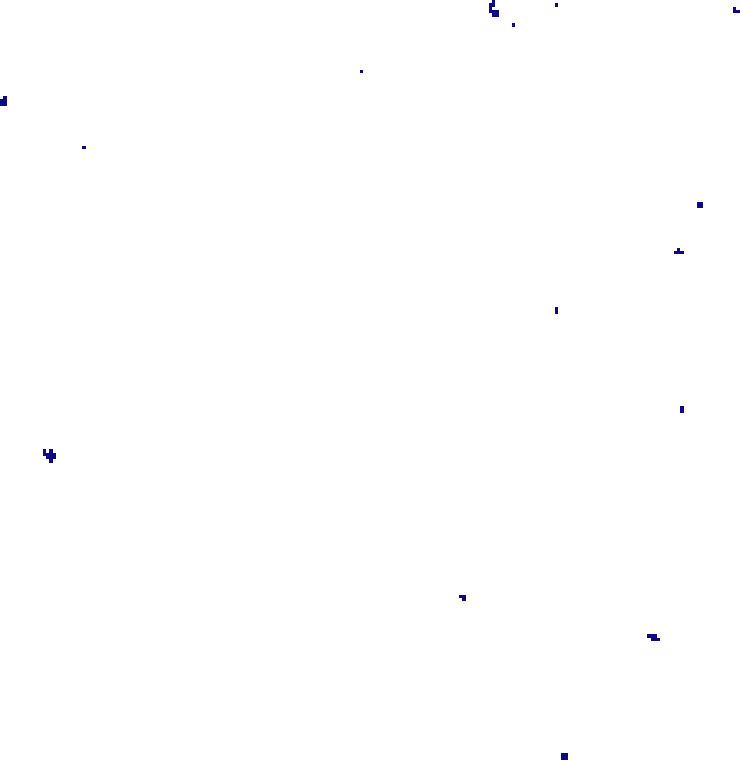
\includegraphics[interpolate=true,width=1.410000in,height=1.446000in]{th_180_450_600-img2.png}}%
\end{pgfscope}%
\begin{pgfscope}%
\pgfpathrectangle{\pgfqpoint{3.741061in}{0.074827in}}{\pgfqpoint{1.590982in}{1.508933in}}%
\pgfusepath{clip}%
\pgfsetbuttcap%
\pgfsetmiterjoin%
\pgfsetlinewidth{1.003750pt}%
\definecolor{currentstroke}{rgb}{0.000000,0.501961,0.000000}%
\pgfsetstrokecolor{currentstroke}%
\pgfsetdash{}{0pt}%
\pgfpathmoveto{\pgfqpoint{3.917104in}{0.659539in}}%
\pgfpathcurveto{\pgfqpoint{3.925441in}{0.659539in}}{\pgfqpoint{3.933437in}{0.662851in}}{\pgfqpoint{3.939332in}{0.668746in}}%
\pgfpathcurveto{\pgfqpoint{3.945228in}{0.674642in}}{\pgfqpoint{3.948540in}{0.682638in}}{\pgfqpoint{3.948540in}{0.690975in}}%
\pgfpathcurveto{\pgfqpoint{3.948540in}{0.699312in}}{\pgfqpoint{3.945228in}{0.707309in}}{\pgfqpoint{3.939332in}{0.713204in}}%
\pgfpathcurveto{\pgfqpoint{3.933437in}{0.719099in}}{\pgfqpoint{3.925441in}{0.722411in}}{\pgfqpoint{3.917104in}{0.722411in}}%
\pgfpathcurveto{\pgfqpoint{3.908767in}{0.722411in}}{\pgfqpoint{3.900770in}{0.719099in}}{\pgfqpoint{3.894875in}{0.713204in}}%
\pgfpathcurveto{\pgfqpoint{3.888980in}{0.707309in}}{\pgfqpoint{3.885668in}{0.699312in}}{\pgfqpoint{3.885668in}{0.690975in}}%
\pgfpathcurveto{\pgfqpoint{3.885668in}{0.682638in}}{\pgfqpoint{3.888980in}{0.674642in}}{\pgfqpoint{3.894875in}{0.668746in}}%
\pgfpathcurveto{\pgfqpoint{3.900770in}{0.662851in}}{\pgfqpoint{3.908767in}{0.659539in}}{\pgfqpoint{3.917104in}{0.659539in}}%
\pgfpathlineto{\pgfqpoint{3.917104in}{0.659539in}}%
\pgfpathclose%
\pgfusepath{stroke}%
\end{pgfscope}%
\begin{pgfscope}%
\pgfpathrectangle{\pgfqpoint{3.741061in}{0.074827in}}{\pgfqpoint{1.590982in}{1.508933in}}%
\pgfusepath{clip}%
\pgfsetbuttcap%
\pgfsetmiterjoin%
\pgfsetlinewidth{1.003750pt}%
\definecolor{currentstroke}{rgb}{0.000000,0.501961,0.000000}%
\pgfsetstrokecolor{currentstroke}%
\pgfsetdash{}{0pt}%
\pgfpathmoveto{\pgfqpoint{4.759592in}{1.508314in}}%
\pgfpathcurveto{\pgfqpoint{4.767928in}{1.508314in}}{\pgfqpoint{4.775925in}{1.511626in}}{\pgfqpoint{4.781820in}{1.517522in}}%
\pgfpathcurveto{\pgfqpoint{4.787715in}{1.523417in}}{\pgfqpoint{4.791028in}{1.531413in}}{\pgfqpoint{4.791028in}{1.539750in}}%
\pgfpathcurveto{\pgfqpoint{4.791028in}{1.548087in}}{\pgfqpoint{4.787715in}{1.556084in}}{\pgfqpoint{4.781820in}{1.561979in}}%
\pgfpathcurveto{\pgfqpoint{4.775925in}{1.567874in}}{\pgfqpoint{4.767928in}{1.571186in}}{\pgfqpoint{4.759592in}{1.571186in}}%
\pgfpathcurveto{\pgfqpoint{4.751255in}{1.571186in}}{\pgfqpoint{4.743258in}{1.567874in}}{\pgfqpoint{4.737363in}{1.561979in}}%
\pgfpathcurveto{\pgfqpoint{4.731468in}{1.556084in}}{\pgfqpoint{4.728155in}{1.548087in}}{\pgfqpoint{4.728155in}{1.539750in}}%
\pgfpathcurveto{\pgfqpoint{4.728155in}{1.531413in}}{\pgfqpoint{4.731468in}{1.523417in}}{\pgfqpoint{4.737363in}{1.517522in}}%
\pgfpathcurveto{\pgfqpoint{4.743258in}{1.511626in}}{\pgfqpoint{4.751255in}{1.508314in}}{\pgfqpoint{4.759592in}{1.508314in}}%
\pgfpathlineto{\pgfqpoint{4.759592in}{1.508314in}}%
\pgfpathclose%
\pgfusepath{stroke}%
\end{pgfscope}%
\begin{pgfscope}%
\pgfpathrectangle{\pgfqpoint{3.741061in}{0.074827in}}{\pgfqpoint{1.590982in}{1.508933in}}%
\pgfusepath{clip}%
\pgfsetbuttcap%
\pgfsetmiterjoin%
\pgfsetlinewidth{1.003750pt}%
\definecolor{currentstroke}{rgb}{0.000000,0.501961,0.000000}%
\pgfsetstrokecolor{currentstroke}%
\pgfsetdash{}{0pt}%
\pgfpathmoveto{\pgfqpoint{5.111676in}{1.043060in}}%
\pgfpathcurveto{\pgfqpoint{5.120013in}{1.043060in}}{\pgfqpoint{5.128010in}{1.046372in}}{\pgfqpoint{5.133905in}{1.052267in}}%
\pgfpathcurveto{\pgfqpoint{5.139800in}{1.058162in}}{\pgfqpoint{5.143112in}{1.066159in}}{\pgfqpoint{5.143112in}{1.074496in}}%
\pgfpathcurveto{\pgfqpoint{5.143112in}{1.082833in}}{\pgfqpoint{5.139800in}{1.090829in}}{\pgfqpoint{5.133905in}{1.096724in}}%
\pgfpathcurveto{\pgfqpoint{5.128010in}{1.102620in}}{\pgfqpoint{5.120013in}{1.105932in}}{\pgfqpoint{5.111676in}{1.105932in}}%
\pgfpathcurveto{\pgfqpoint{5.103339in}{1.105932in}}{\pgfqpoint{5.095342in}{1.102620in}}{\pgfqpoint{5.089447in}{1.096724in}}%
\pgfpathcurveto{\pgfqpoint{5.083552in}{1.090829in}}{\pgfqpoint{5.080240in}{1.082833in}}{\pgfqpoint{5.080240in}{1.074496in}}%
\pgfpathcurveto{\pgfqpoint{5.080240in}{1.066159in}}{\pgfqpoint{5.083552in}{1.058162in}}{\pgfqpoint{5.089447in}{1.052267in}}%
\pgfpathcurveto{\pgfqpoint{5.095342in}{1.046372in}}{\pgfqpoint{5.103339in}{1.043060in}}{\pgfqpoint{5.111676in}{1.043060in}}%
\pgfpathlineto{\pgfqpoint{5.111676in}{1.043060in}}%
\pgfpathclose%
\pgfusepath{stroke}%
\end{pgfscope}%
\begin{pgfscope}%
\pgfpathrectangle{\pgfqpoint{3.741061in}{0.074827in}}{\pgfqpoint{1.590982in}{1.508933in}}%
\pgfusepath{clip}%
\pgfsetbuttcap%
\pgfsetmiterjoin%
\pgfsetlinewidth{1.003750pt}%
\definecolor{currentstroke}{rgb}{0.000000,0.501961,0.000000}%
\pgfsetstrokecolor{currentstroke}%
\pgfsetdash{}{0pt}%
\pgfpathmoveto{\pgfqpoint{4.891623in}{0.087402in}}%
\pgfpathcurveto{\pgfqpoint{4.899960in}{0.087402in}}{\pgfqpoint{4.907957in}{0.090714in}}{\pgfqpoint{4.913852in}{0.096609in}}%
\pgfpathcurveto{\pgfqpoint{4.919747in}{0.102504in}}{\pgfqpoint{4.923059in}{0.110501in}}{\pgfqpoint{4.923059in}{0.118838in}}%
\pgfpathcurveto{\pgfqpoint{4.923059in}{0.127175in}}{\pgfqpoint{4.919747in}{0.135171in}}{\pgfqpoint{4.913852in}{0.141067in}}%
\pgfpathcurveto{\pgfqpoint{4.907957in}{0.146962in}}{\pgfqpoint{4.899960in}{0.150274in}}{\pgfqpoint{4.891623in}{0.150274in}}%
\pgfpathcurveto{\pgfqpoint{4.883286in}{0.150274in}}{\pgfqpoint{4.875290in}{0.146962in}}{\pgfqpoint{4.869395in}{0.141067in}}%
\pgfpathcurveto{\pgfqpoint{4.863499in}{0.135171in}}{\pgfqpoint{4.860187in}{0.127175in}}{\pgfqpoint{4.860187in}{0.118838in}}%
\pgfpathcurveto{\pgfqpoint{4.860187in}{0.110501in}}{\pgfqpoint{4.863499in}{0.102504in}}{\pgfqpoint{4.869395in}{0.096609in}}%
\pgfpathcurveto{\pgfqpoint{4.875290in}{0.090714in}}{\pgfqpoint{4.883286in}{0.087402in}}{\pgfqpoint{4.891623in}{0.087402in}}%
\pgfpathlineto{\pgfqpoint{4.891623in}{0.087402in}}%
\pgfpathclose%
\pgfusepath{stroke}%
\end{pgfscope}%
\begin{pgfscope}%
\pgfpathrectangle{\pgfqpoint{3.741061in}{0.074827in}}{\pgfqpoint{1.590982in}{1.508933in}}%
\pgfusepath{clip}%
\pgfsetbuttcap%
\pgfsetmiterjoin%
\pgfsetlinewidth{1.003750pt}%
\definecolor{currentstroke}{rgb}{0.000000,0.501961,0.000000}%
\pgfsetstrokecolor{currentstroke}%
\pgfsetdash{}{0pt}%
\pgfpathmoveto{\pgfqpoint{4.879049in}{0.936177in}}%
\pgfpathcurveto{\pgfqpoint{4.887386in}{0.936177in}}{\pgfqpoint{4.895382in}{0.939489in}}{\pgfqpoint{4.901277in}{0.945384in}}%
\pgfpathcurveto{\pgfqpoint{4.907173in}{0.951279in}}{\pgfqpoint{4.910485in}{0.959276in}}{\pgfqpoint{4.910485in}{0.967613in}}%
\pgfpathcurveto{\pgfqpoint{4.910485in}{0.975950in}}{\pgfqpoint{4.907173in}{0.983947in}}{\pgfqpoint{4.901277in}{0.989842in}}%
\pgfpathcurveto{\pgfqpoint{4.895382in}{0.995737in}}{\pgfqpoint{4.887386in}{0.999049in}}{\pgfqpoint{4.879049in}{0.999049in}}%
\pgfpathcurveto{\pgfqpoint{4.870712in}{0.999049in}}{\pgfqpoint{4.862715in}{0.995737in}}{\pgfqpoint{4.856820in}{0.989842in}}%
\pgfpathcurveto{\pgfqpoint{4.850925in}{0.983947in}}{\pgfqpoint{4.847613in}{0.975950in}}{\pgfqpoint{4.847613in}{0.967613in}}%
\pgfpathcurveto{\pgfqpoint{4.847613in}{0.959276in}}{\pgfqpoint{4.850925in}{0.951279in}}{\pgfqpoint{4.856820in}{0.945384in}}%
\pgfpathcurveto{\pgfqpoint{4.862715in}{0.939489in}}{\pgfqpoint{4.870712in}{0.936177in}}{\pgfqpoint{4.879049in}{0.936177in}}%
\pgfpathlineto{\pgfqpoint{4.879049in}{0.936177in}}%
\pgfpathclose%
\pgfusepath{stroke}%
\end{pgfscope}%
\begin{pgfscope}%
\pgfpathrectangle{\pgfqpoint{3.741061in}{0.074827in}}{\pgfqpoint{1.590982in}{1.508933in}}%
\pgfusepath{clip}%
\pgfsetbuttcap%
\pgfsetmiterjoin%
\pgfsetlinewidth{1.003750pt}%
\definecolor{currentstroke}{rgb}{0.000000,0.501961,0.000000}%
\pgfsetstrokecolor{currentstroke}%
\pgfsetdash{}{0pt}%
\pgfpathmoveto{\pgfqpoint{5.124250in}{0.753847in}}%
\pgfpathcurveto{\pgfqpoint{5.132587in}{0.753847in}}{\pgfqpoint{5.140584in}{0.757160in}}{\pgfqpoint{5.146479in}{0.763055in}}%
\pgfpathcurveto{\pgfqpoint{5.152374in}{0.768950in}}{\pgfqpoint{5.155687in}{0.776947in}}{\pgfqpoint{5.155687in}{0.785284in}}%
\pgfpathcurveto{\pgfqpoint{5.155687in}{0.793620in}}{\pgfqpoint{5.152374in}{0.801617in}}{\pgfqpoint{5.146479in}{0.807512in}}%
\pgfpathcurveto{\pgfqpoint{5.140584in}{0.813407in}}{\pgfqpoint{5.132587in}{0.816720in}}{\pgfqpoint{5.124250in}{0.816720in}}%
\pgfpathcurveto{\pgfqpoint{5.115913in}{0.816720in}}{\pgfqpoint{5.107917in}{0.813407in}}{\pgfqpoint{5.102022in}{0.807512in}}%
\pgfpathcurveto{\pgfqpoint{5.096127in}{0.801617in}}{\pgfqpoint{5.092814in}{0.793620in}}{\pgfqpoint{5.092814in}{0.785284in}}%
\pgfpathcurveto{\pgfqpoint{5.092814in}{0.776947in}}{\pgfqpoint{5.096127in}{0.768950in}}{\pgfqpoint{5.102022in}{0.763055in}}%
\pgfpathcurveto{\pgfqpoint{5.107917in}{0.757160in}}{\pgfqpoint{5.115913in}{0.753847in}}{\pgfqpoint{5.124250in}{0.753847in}}%
\pgfpathlineto{\pgfqpoint{5.124250in}{0.753847in}}%
\pgfpathclose%
\pgfusepath{stroke}%
\end{pgfscope}%
\begin{pgfscope}%
\pgfpathrectangle{\pgfqpoint{3.741061in}{0.074827in}}{\pgfqpoint{1.590982in}{1.508933in}}%
\pgfusepath{clip}%
\pgfsetbuttcap%
\pgfsetmiterjoin%
\pgfsetlinewidth{1.003750pt}%
\definecolor{currentstroke}{rgb}{0.000000,0.501961,0.000000}%
\pgfsetstrokecolor{currentstroke}%
\pgfsetdash{}{0pt}%
\pgfpathmoveto{\pgfqpoint{5.061378in}{0.313742in}}%
\pgfpathcurveto{\pgfqpoint{5.069715in}{0.313742in}}{\pgfqpoint{5.077712in}{0.317054in}}{\pgfqpoint{5.083607in}{0.322949in}}%
\pgfpathcurveto{\pgfqpoint{5.089502in}{0.328844in}}{\pgfqpoint{5.092814in}{0.336841in}}{\pgfqpoint{5.092814in}{0.345178in}}%
\pgfpathcurveto{\pgfqpoint{5.092814in}{0.353515in}}{\pgfqpoint{5.089502in}{0.361512in}}{\pgfqpoint{5.083607in}{0.367407in}}%
\pgfpathcurveto{\pgfqpoint{5.077712in}{0.373302in}}{\pgfqpoint{5.069715in}{0.376614in}}{\pgfqpoint{5.061378in}{0.376614in}}%
\pgfpathcurveto{\pgfqpoint{5.053041in}{0.376614in}}{\pgfqpoint{5.045045in}{0.373302in}}{\pgfqpoint{5.039150in}{0.367407in}}%
\pgfpathcurveto{\pgfqpoint{5.033254in}{0.361512in}}{\pgfqpoint{5.029942in}{0.353515in}}{\pgfqpoint{5.029942in}{0.345178in}}%
\pgfpathcurveto{\pgfqpoint{5.029942in}{0.336841in}}{\pgfqpoint{5.033254in}{0.328844in}}{\pgfqpoint{5.039150in}{0.322949in}}%
\pgfpathcurveto{\pgfqpoint{5.045045in}{0.317054in}}{\pgfqpoint{5.053041in}{0.313742in}}{\pgfqpoint{5.061378in}{0.313742in}}%
\pgfpathlineto{\pgfqpoint{5.061378in}{0.313742in}}%
\pgfpathclose%
\pgfusepath{stroke}%
\end{pgfscope}%
\begin{pgfscope}%
\pgfpathrectangle{\pgfqpoint{3.741061in}{0.074827in}}{\pgfqpoint{1.590982in}{1.508933in}}%
\pgfusepath{clip}%
\pgfsetbuttcap%
\pgfsetmiterjoin%
\pgfsetlinewidth{1.003750pt}%
\definecolor{currentstroke}{rgb}{0.000000,0.501961,0.000000}%
\pgfsetstrokecolor{currentstroke}%
\pgfsetdash{}{0pt}%
\pgfpathmoveto{\pgfqpoint{3.822795in}{1.338559in}}%
\pgfpathcurveto{\pgfqpoint{3.831132in}{1.338559in}}{\pgfqpoint{3.839129in}{1.341871in}}{\pgfqpoint{3.845024in}{1.347767in}}%
\pgfpathcurveto{\pgfqpoint{3.850919in}{1.353662in}}{\pgfqpoint{3.854231in}{1.361658in}}{\pgfqpoint{3.854231in}{1.369995in}}%
\pgfpathcurveto{\pgfqpoint{3.854231in}{1.378332in}}{\pgfqpoint{3.850919in}{1.386329in}}{\pgfqpoint{3.845024in}{1.392224in}}%
\pgfpathcurveto{\pgfqpoint{3.839129in}{1.398119in}}{\pgfqpoint{3.831132in}{1.401431in}}{\pgfqpoint{3.822795in}{1.401431in}}%
\pgfpathcurveto{\pgfqpoint{3.814458in}{1.401431in}}{\pgfqpoint{3.806462in}{1.398119in}}{\pgfqpoint{3.800567in}{1.392224in}}%
\pgfpathcurveto{\pgfqpoint{3.794672in}{1.386329in}}{\pgfqpoint{3.791359in}{1.378332in}}{\pgfqpoint{3.791359in}{1.369995in}}%
\pgfpathcurveto{\pgfqpoint{3.791359in}{1.361658in}}{\pgfqpoint{3.794672in}{1.353662in}}{\pgfqpoint{3.800567in}{1.347767in}}%
\pgfpathcurveto{\pgfqpoint{3.806462in}{1.341871in}}{\pgfqpoint{3.814458in}{1.338559in}}{\pgfqpoint{3.822795in}{1.338559in}}%
\pgfpathlineto{\pgfqpoint{3.822795in}{1.338559in}}%
\pgfpathclose%
\pgfusepath{stroke}%
\end{pgfscope}%
\begin{pgfscope}%
\pgfpathrectangle{\pgfqpoint{3.741061in}{0.074827in}}{\pgfqpoint{1.590982in}{1.508933in}}%
\pgfusepath{clip}%
\pgfsetbuttcap%
\pgfsetmiterjoin%
\pgfsetlinewidth{1.003750pt}%
\definecolor{currentstroke}{rgb}{0.000000,0.501961,0.000000}%
\pgfsetstrokecolor{currentstroke}%
\pgfsetdash{}{0pt}%
\pgfpathmoveto{\pgfqpoint{4.696719in}{0.389188in}}%
\pgfpathcurveto{\pgfqpoint{4.705056in}{0.389188in}}{\pgfqpoint{4.713053in}{0.392501in}}{\pgfqpoint{4.718948in}{0.398396in}}%
\pgfpathcurveto{\pgfqpoint{4.724843in}{0.404291in}}{\pgfqpoint{4.728155in}{0.412288in}}{\pgfqpoint{4.728155in}{0.420625in}}%
\pgfpathcurveto{\pgfqpoint{4.728155in}{0.428962in}}{\pgfqpoint{4.724843in}{0.436958in}}{\pgfqpoint{4.718948in}{0.442853in}}%
\pgfpathcurveto{\pgfqpoint{4.713053in}{0.448748in}}{\pgfqpoint{4.705056in}{0.452061in}}{\pgfqpoint{4.696719in}{0.452061in}}%
\pgfpathcurveto{\pgfqpoint{4.688382in}{0.452061in}}{\pgfqpoint{4.680386in}{0.448748in}}{\pgfqpoint{4.674491in}{0.442853in}}%
\pgfpathcurveto{\pgfqpoint{4.668596in}{0.436958in}}{\pgfqpoint{4.665283in}{0.428962in}}{\pgfqpoint{4.665283in}{0.420625in}}%
\pgfpathcurveto{\pgfqpoint{4.665283in}{0.412288in}}{\pgfqpoint{4.668596in}{0.404291in}}{\pgfqpoint{4.674491in}{0.398396in}}%
\pgfpathcurveto{\pgfqpoint{4.680386in}{0.392501in}}{\pgfqpoint{4.688382in}{0.389188in}}{\pgfqpoint{4.696719in}{0.389188in}}%
\pgfpathlineto{\pgfqpoint{4.696719in}{0.389188in}}%
\pgfpathclose%
\pgfusepath{stroke}%
\end{pgfscope}%
\begin{pgfscope}%
\pgfpathrectangle{\pgfqpoint{3.741061in}{0.074827in}}{\pgfqpoint{1.590982in}{1.508933in}}%
\pgfusepath{clip}%
\pgfsetbuttcap%
\pgfsetmiterjoin%
\pgfsetlinewidth{1.003750pt}%
\definecolor{currentstroke}{rgb}{0.000000,0.501961,0.000000}%
\pgfsetstrokecolor{currentstroke}%
\pgfsetdash{}{0pt}%
\pgfpathmoveto{\pgfqpoint{5.224846in}{1.502027in}}%
\pgfpathcurveto{\pgfqpoint{5.233183in}{1.502027in}}{\pgfqpoint{5.241180in}{1.505339in}}{\pgfqpoint{5.247075in}{1.511234in}}%
\pgfpathcurveto{\pgfqpoint{5.252970in}{1.517129in}}{\pgfqpoint{5.256282in}{1.525126in}}{\pgfqpoint{5.256282in}{1.533463in}}%
\pgfpathcurveto{\pgfqpoint{5.256282in}{1.541800in}}{\pgfqpoint{5.252970in}{1.549797in}}{\pgfqpoint{5.247075in}{1.555692in}}%
\pgfpathcurveto{\pgfqpoint{5.241180in}{1.561587in}}{\pgfqpoint{5.233183in}{1.564899in}}{\pgfqpoint{5.224846in}{1.564899in}}%
\pgfpathcurveto{\pgfqpoint{5.216509in}{1.564899in}}{\pgfqpoint{5.208512in}{1.561587in}}{\pgfqpoint{5.202617in}{1.555692in}}%
\pgfpathcurveto{\pgfqpoint{5.196722in}{1.549797in}}{\pgfqpoint{5.193410in}{1.541800in}}{\pgfqpoint{5.193410in}{1.533463in}}%
\pgfpathcurveto{\pgfqpoint{5.193410in}{1.525126in}}{\pgfqpoint{5.196722in}{1.517129in}}{\pgfqpoint{5.202617in}{1.511234in}}%
\pgfpathcurveto{\pgfqpoint{5.208512in}{1.505339in}}{\pgfqpoint{5.216509in}{1.502027in}}{\pgfqpoint{5.224846in}{1.502027in}}%
\pgfpathlineto{\pgfqpoint{5.224846in}{1.502027in}}%
\pgfpathclose%
\pgfusepath{stroke}%
\end{pgfscope}%
\begin{pgfscope}%
\pgfpathrectangle{\pgfqpoint{3.741061in}{0.074827in}}{\pgfqpoint{1.590982in}{1.508933in}}%
\pgfusepath{clip}%
\pgfsetbuttcap%
\pgfsetmiterjoin%
\pgfsetlinewidth{1.003750pt}%
\definecolor{currentstroke}{rgb}{0.000000,0.501961,0.000000}%
\pgfsetstrokecolor{currentstroke}%
\pgfsetdash{}{0pt}%
\pgfpathmoveto{\pgfqpoint{5.155687in}{1.137368in}}%
\pgfpathcurveto{\pgfqpoint{5.164024in}{1.137368in}}{\pgfqpoint{5.172020in}{1.140680in}}{\pgfqpoint{5.177915in}{1.146575in}}%
\pgfpathcurveto{\pgfqpoint{5.183810in}{1.152471in}}{\pgfqpoint{5.187123in}{1.160467in}}{\pgfqpoint{5.187123in}{1.168804in}}%
\pgfpathcurveto{\pgfqpoint{5.187123in}{1.177141in}}{\pgfqpoint{5.183810in}{1.185138in}}{\pgfqpoint{5.177915in}{1.191033in}}%
\pgfpathcurveto{\pgfqpoint{5.172020in}{1.196928in}}{\pgfqpoint{5.164024in}{1.200240in}}{\pgfqpoint{5.155687in}{1.200240in}}%
\pgfpathcurveto{\pgfqpoint{5.147350in}{1.200240in}}{\pgfqpoint{5.139353in}{1.196928in}}{\pgfqpoint{5.133458in}{1.191033in}}%
\pgfpathcurveto{\pgfqpoint{5.127563in}{1.185138in}}{\pgfqpoint{5.124250in}{1.177141in}}{\pgfqpoint{5.124250in}{1.168804in}}%
\pgfpathcurveto{\pgfqpoint{5.124250in}{1.160467in}}{\pgfqpoint{5.127563in}{1.152471in}}{\pgfqpoint{5.133458in}{1.146575in}}%
\pgfpathcurveto{\pgfqpoint{5.139353in}{1.140680in}}{\pgfqpoint{5.147350in}{1.137368in}}{\pgfqpoint{5.155687in}{1.137368in}}%
\pgfpathlineto{\pgfqpoint{5.155687in}{1.137368in}}%
\pgfpathclose%
\pgfusepath{stroke}%
\end{pgfscope}%
\begin{pgfscope}%
\pgfsetrectcap%
\pgfsetmiterjoin%
\pgfsetlinewidth{0.803000pt}%
\definecolor{currentstroke}{rgb}{0.000000,0.000000,0.000000}%
\pgfsetstrokecolor{currentstroke}%
\pgfsetdash{}{0pt}%
\pgfpathmoveto{\pgfqpoint{3.741061in}{0.074827in}}%
\pgfpathlineto{\pgfqpoint{3.741061in}{1.583761in}}%
\pgfusepath{stroke}%
\end{pgfscope}%
\begin{pgfscope}%
\pgfsetrectcap%
\pgfsetmiterjoin%
\pgfsetlinewidth{0.803000pt}%
\definecolor{currentstroke}{rgb}{0.000000,0.000000,0.000000}%
\pgfsetstrokecolor{currentstroke}%
\pgfsetdash{}{0pt}%
\pgfpathmoveto{\pgfqpoint{5.332043in}{0.074827in}}%
\pgfpathlineto{\pgfqpoint{5.332043in}{1.583761in}}%
\pgfusepath{stroke}%
\end{pgfscope}%
\begin{pgfscope}%
\pgfsetrectcap%
\pgfsetmiterjoin%
\pgfsetlinewidth{0.803000pt}%
\definecolor{currentstroke}{rgb}{0.000000,0.000000,0.000000}%
\pgfsetstrokecolor{currentstroke}%
\pgfsetdash{}{0pt}%
\pgfpathmoveto{\pgfqpoint{3.741061in}{0.074827in}}%
\pgfpathlineto{\pgfqpoint{5.332043in}{0.074827in}}%
\pgfusepath{stroke}%
\end{pgfscope}%
\begin{pgfscope}%
\pgfsetrectcap%
\pgfsetmiterjoin%
\pgfsetlinewidth{0.803000pt}%
\definecolor{currentstroke}{rgb}{0.000000,0.000000,0.000000}%
\pgfsetstrokecolor{currentstroke}%
\pgfsetdash{}{0pt}%
\pgfpathmoveto{\pgfqpoint{3.741061in}{1.583761in}}%
\pgfpathlineto{\pgfqpoint{5.332043in}{1.583761in}}%
\pgfusepath{stroke}%
\end{pgfscope}%
\begin{pgfscope}%
\definecolor{textcolor}{rgb}{0.000000,0.000000,0.000000}%
\pgfsetstrokecolor{textcolor}%
\pgfsetfillcolor{textcolor}%
\pgftext[x=3.581963in,y=1.734654in,left,base]{\color{textcolor}\rmfamily\fontsize{10.000000}{12.000000}\selectfont (c)}%
\end{pgfscope}%
\begin{pgfscope}%
\pgfsetbuttcap%
\pgfsetmiterjoin%
\definecolor{currentfill}{rgb}{1.000000,1.000000,1.000000}%
\pgfsetfillcolor{currentfill}%
\pgfsetlinewidth{0.000000pt}%
\definecolor{currentstroke}{rgb}{0.000000,0.000000,0.000000}%
\pgfsetstrokecolor{currentstroke}%
\pgfsetstrokeopacity{0.000000}%
\pgfsetdash{}{0pt}%
\pgfpathmoveto{\pgfqpoint{5.532043in}{0.074827in}}%
\pgfpathlineto{\pgfqpoint{5.643412in}{0.074827in}}%
\pgfpathlineto{\pgfqpoint{5.643412in}{1.583761in}}%
\pgfpathlineto{\pgfqpoint{5.532043in}{1.583761in}}%
\pgfpathlineto{\pgfqpoint{5.532043in}{0.074827in}}%
\pgfpathclose%
\pgfusepath{fill}%
\end{pgfscope}%
\begin{pgfscope}%
\pgfpathrectangle{\pgfqpoint{5.532043in}{0.074827in}}{\pgfqpoint{0.111369in}{1.508933in}}%
\pgfusepath{clip}%
\pgfsetbuttcap%
\pgfsetmiterjoin%
\definecolor{currentfill}{rgb}{1.000000,1.000000,1.000000}%
\pgfsetfillcolor{currentfill}%
\pgfsetlinewidth{0.010037pt}%
\definecolor{currentstroke}{rgb}{1.000000,1.000000,1.000000}%
\pgfsetstrokecolor{currentstroke}%
\pgfsetdash{}{0pt}%
\pgfusepath{stroke,fill}%
\end{pgfscope}%
\begin{pgfscope}%
\pgfsys@transformshift{5.532000in}{0.074795in}%
\pgftext[left,bottom]{
\includegraphics[interpolate=true,width=0.112000in,height=1.510000in]{th_180_450_600-img3.png}}%
\end{pgfscope}%
\begin{pgfscope}%
\pgfsetbuttcap%
\pgfsetroundjoin%
\definecolor{currentfill}{rgb}{0.000000,0.000000,0.000000}%
\pgfsetfillcolor{currentfill}%
\pgfsetlinewidth{0.803000pt}%
\definecolor{currentstroke}{rgb}{0.000000,0.000000,0.000000}%
\pgfsetstrokecolor{currentstroke}%
\pgfsetdash{}{0pt}%
\pgfsys@defobject{currentmarker}{\pgfqpoint{0.000000in}{0.000000in}}{\pgfqpoint{0.048611in}{0.000000in}}{%
\pgfpathmoveto{\pgfqpoint{0.000000in}{0.000000in}}%
\pgfpathlineto{\pgfqpoint{0.048611in}{0.000000in}}%
\pgfusepath{stroke,fill}%
}%
\begin{pgfscope}%
\pgfsys@transformshift{5.643412in}{0.074827in}%
\pgfsys@useobject{currentmarker}{}%
\end{pgfscope}%
\end{pgfscope}%
\begin{pgfscope}%
\definecolor{textcolor}{rgb}{0.000000,0.000000,0.000000}%
\pgfsetstrokecolor{textcolor}%
\pgfsetfillcolor{textcolor}%
\pgftext[x=5.740634in, y=0.027000in, left, base]{\color{textcolor}\rmfamily\fontsize{10.000000}{12.000000}\selectfont 1}%
\end{pgfscope}%
\begin{pgfscope}%
\pgfsetbuttcap%
\pgfsetroundjoin%
\definecolor{currentfill}{rgb}{0.000000,0.000000,0.000000}%
\pgfsetfillcolor{currentfill}%
\pgfsetlinewidth{0.803000pt}%
\definecolor{currentstroke}{rgb}{0.000000,0.000000,0.000000}%
\pgfsetstrokecolor{currentstroke}%
\pgfsetdash{}{0pt}%
\pgfsys@defobject{currentmarker}{\pgfqpoint{0.000000in}{0.000000in}}{\pgfqpoint{0.048611in}{0.000000in}}{%
\pgfpathmoveto{\pgfqpoint{0.000000in}{0.000000in}}%
\pgfpathlineto{\pgfqpoint{0.048611in}{0.000000in}}%
\pgfusepath{stroke,fill}%
}%
\begin{pgfscope}%
\pgfsys@transformshift{5.643412in}{0.577805in}%
\pgfsys@useobject{currentmarker}{}%
\end{pgfscope}%
\end{pgfscope}%
\begin{pgfscope}%
\definecolor{textcolor}{rgb}{0.000000,0.000000,0.000000}%
\pgfsetstrokecolor{textcolor}%
\pgfsetfillcolor{textcolor}%
\pgftext[x=5.740634in, y=0.529977in, left, base]{\color{textcolor}\rmfamily\fontsize{10.000000}{12.000000}\selectfont 10}%
\end{pgfscope}%
\begin{pgfscope}%
\pgfsetbuttcap%
\pgfsetroundjoin%
\definecolor{currentfill}{rgb}{0.000000,0.000000,0.000000}%
\pgfsetfillcolor{currentfill}%
\pgfsetlinewidth{0.803000pt}%
\definecolor{currentstroke}{rgb}{0.000000,0.000000,0.000000}%
\pgfsetstrokecolor{currentstroke}%
\pgfsetdash{}{0pt}%
\pgfsys@defobject{currentmarker}{\pgfqpoint{0.000000in}{0.000000in}}{\pgfqpoint{0.048611in}{0.000000in}}{%
\pgfpathmoveto{\pgfqpoint{0.000000in}{0.000000in}}%
\pgfpathlineto{\pgfqpoint{0.048611in}{0.000000in}}%
\pgfusepath{stroke,fill}%
}%
\begin{pgfscope}%
\pgfsys@transformshift{5.643412in}{1.080783in}%
\pgfsys@useobject{currentmarker}{}%
\end{pgfscope}%
\end{pgfscope}%
\begin{pgfscope}%
\definecolor{textcolor}{rgb}{0.000000,0.000000,0.000000}%
\pgfsetstrokecolor{textcolor}%
\pgfsetfillcolor{textcolor}%
\pgftext[x=5.740634in, y=1.032955in, left, base]{\color{textcolor}\rmfamily\fontsize{10.000000}{12.000000}\selectfont 100}%
\end{pgfscope}%
\begin{pgfscope}%
\pgfsetbuttcap%
\pgfsetroundjoin%
\definecolor{currentfill}{rgb}{0.000000,0.000000,0.000000}%
\pgfsetfillcolor{currentfill}%
\pgfsetlinewidth{0.803000pt}%
\definecolor{currentstroke}{rgb}{0.000000,0.000000,0.000000}%
\pgfsetstrokecolor{currentstroke}%
\pgfsetdash{}{0pt}%
\pgfsys@defobject{currentmarker}{\pgfqpoint{0.000000in}{0.000000in}}{\pgfqpoint{0.048611in}{0.000000in}}{%
\pgfpathmoveto{\pgfqpoint{0.000000in}{0.000000in}}%
\pgfpathlineto{\pgfqpoint{0.048611in}{0.000000in}}%
\pgfusepath{stroke,fill}%
}%
\begin{pgfscope}%
\pgfsys@transformshift{5.643412in}{1.583761in}%
\pgfsys@useobject{currentmarker}{}%
\end{pgfscope}%
\end{pgfscope}%
\begin{pgfscope}%
\definecolor{textcolor}{rgb}{0.000000,0.000000,0.000000}%
\pgfsetstrokecolor{textcolor}%
\pgfsetfillcolor{textcolor}%
\pgftext[x=5.740634in, y=1.535933in, left, base]{\color{textcolor}\rmfamily\fontsize{10.000000}{12.000000}\selectfont 1000}%
\end{pgfscope}%
\begin{pgfscope}%
\pgfsetbuttcap%
\pgfsetroundjoin%
\definecolor{currentfill}{rgb}{0.000000,0.000000,0.000000}%
\pgfsetfillcolor{currentfill}%
\pgfsetlinewidth{0.602250pt}%
\definecolor{currentstroke}{rgb}{0.000000,0.000000,0.000000}%
\pgfsetstrokecolor{currentstroke}%
\pgfsetdash{}{0pt}%
\pgfsys@defobject{currentmarker}{\pgfqpoint{0.000000in}{0.000000in}}{\pgfqpoint{0.027778in}{0.000000in}}{%
\pgfpathmoveto{\pgfqpoint{0.000000in}{0.000000in}}%
\pgfpathlineto{\pgfqpoint{0.027778in}{0.000000in}}%
\pgfusepath{stroke,fill}%
}%
\begin{pgfscope}%
\pgfsys@transformshift{5.643412in}{0.226239in}%
\pgfsys@useobject{currentmarker}{}%
\end{pgfscope}%
\end{pgfscope}%
\begin{pgfscope}%
\pgfsetbuttcap%
\pgfsetroundjoin%
\definecolor{currentfill}{rgb}{0.000000,0.000000,0.000000}%
\pgfsetfillcolor{currentfill}%
\pgfsetlinewidth{0.602250pt}%
\definecolor{currentstroke}{rgb}{0.000000,0.000000,0.000000}%
\pgfsetstrokecolor{currentstroke}%
\pgfsetdash{}{0pt}%
\pgfsys@defobject{currentmarker}{\pgfqpoint{0.000000in}{0.000000in}}{\pgfqpoint{0.027778in}{0.000000in}}{%
\pgfpathmoveto{\pgfqpoint{0.000000in}{0.000000in}}%
\pgfpathlineto{\pgfqpoint{0.027778in}{0.000000in}}%
\pgfusepath{stroke,fill}%
}%
\begin{pgfscope}%
\pgfsys@transformshift{5.643412in}{0.314809in}%
\pgfsys@useobject{currentmarker}{}%
\end{pgfscope}%
\end{pgfscope}%
\begin{pgfscope}%
\pgfsetbuttcap%
\pgfsetroundjoin%
\definecolor{currentfill}{rgb}{0.000000,0.000000,0.000000}%
\pgfsetfillcolor{currentfill}%
\pgfsetlinewidth{0.602250pt}%
\definecolor{currentstroke}{rgb}{0.000000,0.000000,0.000000}%
\pgfsetstrokecolor{currentstroke}%
\pgfsetdash{}{0pt}%
\pgfsys@defobject{currentmarker}{\pgfqpoint{0.000000in}{0.000000in}}{\pgfqpoint{0.027778in}{0.000000in}}{%
\pgfpathmoveto{\pgfqpoint{0.000000in}{0.000000in}}%
\pgfpathlineto{\pgfqpoint{0.027778in}{0.000000in}}%
\pgfusepath{stroke,fill}%
}%
\begin{pgfscope}%
\pgfsys@transformshift{5.643412in}{0.377650in}%
\pgfsys@useobject{currentmarker}{}%
\end{pgfscope}%
\end{pgfscope}%
\begin{pgfscope}%
\pgfsetbuttcap%
\pgfsetroundjoin%
\definecolor{currentfill}{rgb}{0.000000,0.000000,0.000000}%
\pgfsetfillcolor{currentfill}%
\pgfsetlinewidth{0.602250pt}%
\definecolor{currentstroke}{rgb}{0.000000,0.000000,0.000000}%
\pgfsetstrokecolor{currentstroke}%
\pgfsetdash{}{0pt}%
\pgfsys@defobject{currentmarker}{\pgfqpoint{0.000000in}{0.000000in}}{\pgfqpoint{0.027778in}{0.000000in}}{%
\pgfpathmoveto{\pgfqpoint{0.000000in}{0.000000in}}%
\pgfpathlineto{\pgfqpoint{0.027778in}{0.000000in}}%
\pgfusepath{stroke,fill}%
}%
\begin{pgfscope}%
\pgfsys@transformshift{5.643412in}{0.426394in}%
\pgfsys@useobject{currentmarker}{}%
\end{pgfscope}%
\end{pgfscope}%
\begin{pgfscope}%
\pgfsetbuttcap%
\pgfsetroundjoin%
\definecolor{currentfill}{rgb}{0.000000,0.000000,0.000000}%
\pgfsetfillcolor{currentfill}%
\pgfsetlinewidth{0.602250pt}%
\definecolor{currentstroke}{rgb}{0.000000,0.000000,0.000000}%
\pgfsetstrokecolor{currentstroke}%
\pgfsetdash{}{0pt}%
\pgfsys@defobject{currentmarker}{\pgfqpoint{0.000000in}{0.000000in}}{\pgfqpoint{0.027778in}{0.000000in}}{%
\pgfpathmoveto{\pgfqpoint{0.000000in}{0.000000in}}%
\pgfpathlineto{\pgfqpoint{0.027778in}{0.000000in}}%
\pgfusepath{stroke,fill}%
}%
\begin{pgfscope}%
\pgfsys@transformshift{5.643412in}{0.466220in}%
\pgfsys@useobject{currentmarker}{}%
\end{pgfscope}%
\end{pgfscope}%
\begin{pgfscope}%
\pgfsetbuttcap%
\pgfsetroundjoin%
\definecolor{currentfill}{rgb}{0.000000,0.000000,0.000000}%
\pgfsetfillcolor{currentfill}%
\pgfsetlinewidth{0.602250pt}%
\definecolor{currentstroke}{rgb}{0.000000,0.000000,0.000000}%
\pgfsetstrokecolor{currentstroke}%
\pgfsetdash{}{0pt}%
\pgfsys@defobject{currentmarker}{\pgfqpoint{0.000000in}{0.000000in}}{\pgfqpoint{0.027778in}{0.000000in}}{%
\pgfpathmoveto{\pgfqpoint{0.000000in}{0.000000in}}%
\pgfpathlineto{\pgfqpoint{0.027778in}{0.000000in}}%
\pgfusepath{stroke,fill}%
}%
\begin{pgfscope}%
\pgfsys@transformshift{5.643412in}{0.499893in}%
\pgfsys@useobject{currentmarker}{}%
\end{pgfscope}%
\end{pgfscope}%
\begin{pgfscope}%
\pgfsetbuttcap%
\pgfsetroundjoin%
\definecolor{currentfill}{rgb}{0.000000,0.000000,0.000000}%
\pgfsetfillcolor{currentfill}%
\pgfsetlinewidth{0.602250pt}%
\definecolor{currentstroke}{rgb}{0.000000,0.000000,0.000000}%
\pgfsetstrokecolor{currentstroke}%
\pgfsetdash{}{0pt}%
\pgfsys@defobject{currentmarker}{\pgfqpoint{0.000000in}{0.000000in}}{\pgfqpoint{0.027778in}{0.000000in}}{%
\pgfpathmoveto{\pgfqpoint{0.000000in}{0.000000in}}%
\pgfpathlineto{\pgfqpoint{0.027778in}{0.000000in}}%
\pgfusepath{stroke,fill}%
}%
\begin{pgfscope}%
\pgfsys@transformshift{5.643412in}{0.529062in}%
\pgfsys@useobject{currentmarker}{}%
\end{pgfscope}%
\end{pgfscope}%
\begin{pgfscope}%
\pgfsetbuttcap%
\pgfsetroundjoin%
\definecolor{currentfill}{rgb}{0.000000,0.000000,0.000000}%
\pgfsetfillcolor{currentfill}%
\pgfsetlinewidth{0.602250pt}%
\definecolor{currentstroke}{rgb}{0.000000,0.000000,0.000000}%
\pgfsetstrokecolor{currentstroke}%
\pgfsetdash{}{0pt}%
\pgfsys@defobject{currentmarker}{\pgfqpoint{0.000000in}{0.000000in}}{\pgfqpoint{0.027778in}{0.000000in}}{%
\pgfpathmoveto{\pgfqpoint{0.000000in}{0.000000in}}%
\pgfpathlineto{\pgfqpoint{0.027778in}{0.000000in}}%
\pgfusepath{stroke,fill}%
}%
\begin{pgfscope}%
\pgfsys@transformshift{5.643412in}{0.554790in}%
\pgfsys@useobject{currentmarker}{}%
\end{pgfscope}%
\end{pgfscope}%
\begin{pgfscope}%
\pgfsetbuttcap%
\pgfsetroundjoin%
\definecolor{currentfill}{rgb}{0.000000,0.000000,0.000000}%
\pgfsetfillcolor{currentfill}%
\pgfsetlinewidth{0.602250pt}%
\definecolor{currentstroke}{rgb}{0.000000,0.000000,0.000000}%
\pgfsetstrokecolor{currentstroke}%
\pgfsetdash{}{0pt}%
\pgfsys@defobject{currentmarker}{\pgfqpoint{0.000000in}{0.000000in}}{\pgfqpoint{0.027778in}{0.000000in}}{%
\pgfpathmoveto{\pgfqpoint{0.000000in}{0.000000in}}%
\pgfpathlineto{\pgfqpoint{0.027778in}{0.000000in}}%
\pgfusepath{stroke,fill}%
}%
\begin{pgfscope}%
\pgfsys@transformshift{5.643412in}{0.729217in}%
\pgfsys@useobject{currentmarker}{}%
\end{pgfscope}%
\end{pgfscope}%
\begin{pgfscope}%
\pgfsetbuttcap%
\pgfsetroundjoin%
\definecolor{currentfill}{rgb}{0.000000,0.000000,0.000000}%
\pgfsetfillcolor{currentfill}%
\pgfsetlinewidth{0.602250pt}%
\definecolor{currentstroke}{rgb}{0.000000,0.000000,0.000000}%
\pgfsetstrokecolor{currentstroke}%
\pgfsetdash{}{0pt}%
\pgfsys@defobject{currentmarker}{\pgfqpoint{0.000000in}{0.000000in}}{\pgfqpoint{0.027778in}{0.000000in}}{%
\pgfpathmoveto{\pgfqpoint{0.000000in}{0.000000in}}%
\pgfpathlineto{\pgfqpoint{0.027778in}{0.000000in}}%
\pgfusepath{stroke,fill}%
}%
\begin{pgfscope}%
\pgfsys@transformshift{5.643412in}{0.817787in}%
\pgfsys@useobject{currentmarker}{}%
\end{pgfscope}%
\end{pgfscope}%
\begin{pgfscope}%
\pgfsetbuttcap%
\pgfsetroundjoin%
\definecolor{currentfill}{rgb}{0.000000,0.000000,0.000000}%
\pgfsetfillcolor{currentfill}%
\pgfsetlinewidth{0.602250pt}%
\definecolor{currentstroke}{rgb}{0.000000,0.000000,0.000000}%
\pgfsetstrokecolor{currentstroke}%
\pgfsetdash{}{0pt}%
\pgfsys@defobject{currentmarker}{\pgfqpoint{0.000000in}{0.000000in}}{\pgfqpoint{0.027778in}{0.000000in}}{%
\pgfpathmoveto{\pgfqpoint{0.000000in}{0.000000in}}%
\pgfpathlineto{\pgfqpoint{0.027778in}{0.000000in}}%
\pgfusepath{stroke,fill}%
}%
\begin{pgfscope}%
\pgfsys@transformshift{5.643412in}{0.880628in}%
\pgfsys@useobject{currentmarker}{}%
\end{pgfscope}%
\end{pgfscope}%
\begin{pgfscope}%
\pgfsetbuttcap%
\pgfsetroundjoin%
\definecolor{currentfill}{rgb}{0.000000,0.000000,0.000000}%
\pgfsetfillcolor{currentfill}%
\pgfsetlinewidth{0.602250pt}%
\definecolor{currentstroke}{rgb}{0.000000,0.000000,0.000000}%
\pgfsetstrokecolor{currentstroke}%
\pgfsetdash{}{0pt}%
\pgfsys@defobject{currentmarker}{\pgfqpoint{0.000000in}{0.000000in}}{\pgfqpoint{0.027778in}{0.000000in}}{%
\pgfpathmoveto{\pgfqpoint{0.000000in}{0.000000in}}%
\pgfpathlineto{\pgfqpoint{0.027778in}{0.000000in}}%
\pgfusepath{stroke,fill}%
}%
\begin{pgfscope}%
\pgfsys@transformshift{5.643412in}{0.929372in}%
\pgfsys@useobject{currentmarker}{}%
\end{pgfscope}%
\end{pgfscope}%
\begin{pgfscope}%
\pgfsetbuttcap%
\pgfsetroundjoin%
\definecolor{currentfill}{rgb}{0.000000,0.000000,0.000000}%
\pgfsetfillcolor{currentfill}%
\pgfsetlinewidth{0.602250pt}%
\definecolor{currentstroke}{rgb}{0.000000,0.000000,0.000000}%
\pgfsetstrokecolor{currentstroke}%
\pgfsetdash{}{0pt}%
\pgfsys@defobject{currentmarker}{\pgfqpoint{0.000000in}{0.000000in}}{\pgfqpoint{0.027778in}{0.000000in}}{%
\pgfpathmoveto{\pgfqpoint{0.000000in}{0.000000in}}%
\pgfpathlineto{\pgfqpoint{0.027778in}{0.000000in}}%
\pgfusepath{stroke,fill}%
}%
\begin{pgfscope}%
\pgfsys@transformshift{5.643412in}{0.969198in}%
\pgfsys@useobject{currentmarker}{}%
\end{pgfscope}%
\end{pgfscope}%
\begin{pgfscope}%
\pgfsetbuttcap%
\pgfsetroundjoin%
\definecolor{currentfill}{rgb}{0.000000,0.000000,0.000000}%
\pgfsetfillcolor{currentfill}%
\pgfsetlinewidth{0.602250pt}%
\definecolor{currentstroke}{rgb}{0.000000,0.000000,0.000000}%
\pgfsetstrokecolor{currentstroke}%
\pgfsetdash{}{0pt}%
\pgfsys@defobject{currentmarker}{\pgfqpoint{0.000000in}{0.000000in}}{\pgfqpoint{0.027778in}{0.000000in}}{%
\pgfpathmoveto{\pgfqpoint{0.000000in}{0.000000in}}%
\pgfpathlineto{\pgfqpoint{0.027778in}{0.000000in}}%
\pgfusepath{stroke,fill}%
}%
\begin{pgfscope}%
\pgfsys@transformshift{5.643412in}{1.002871in}%
\pgfsys@useobject{currentmarker}{}%
\end{pgfscope}%
\end{pgfscope}%
\begin{pgfscope}%
\pgfsetbuttcap%
\pgfsetroundjoin%
\definecolor{currentfill}{rgb}{0.000000,0.000000,0.000000}%
\pgfsetfillcolor{currentfill}%
\pgfsetlinewidth{0.602250pt}%
\definecolor{currentstroke}{rgb}{0.000000,0.000000,0.000000}%
\pgfsetstrokecolor{currentstroke}%
\pgfsetdash{}{0pt}%
\pgfsys@defobject{currentmarker}{\pgfqpoint{0.000000in}{0.000000in}}{\pgfqpoint{0.027778in}{0.000000in}}{%
\pgfpathmoveto{\pgfqpoint{0.000000in}{0.000000in}}%
\pgfpathlineto{\pgfqpoint{0.027778in}{0.000000in}}%
\pgfusepath{stroke,fill}%
}%
\begin{pgfscope}%
\pgfsys@transformshift{5.643412in}{1.032039in}%
\pgfsys@useobject{currentmarker}{}%
\end{pgfscope}%
\end{pgfscope}%
\begin{pgfscope}%
\pgfsetbuttcap%
\pgfsetroundjoin%
\definecolor{currentfill}{rgb}{0.000000,0.000000,0.000000}%
\pgfsetfillcolor{currentfill}%
\pgfsetlinewidth{0.602250pt}%
\definecolor{currentstroke}{rgb}{0.000000,0.000000,0.000000}%
\pgfsetstrokecolor{currentstroke}%
\pgfsetdash{}{0pt}%
\pgfsys@defobject{currentmarker}{\pgfqpoint{0.000000in}{0.000000in}}{\pgfqpoint{0.027778in}{0.000000in}}{%
\pgfpathmoveto{\pgfqpoint{0.000000in}{0.000000in}}%
\pgfpathlineto{\pgfqpoint{0.027778in}{0.000000in}}%
\pgfusepath{stroke,fill}%
}%
\begin{pgfscope}%
\pgfsys@transformshift{5.643412in}{1.057768in}%
\pgfsys@useobject{currentmarker}{}%
\end{pgfscope}%
\end{pgfscope}%
\begin{pgfscope}%
\pgfsetbuttcap%
\pgfsetroundjoin%
\definecolor{currentfill}{rgb}{0.000000,0.000000,0.000000}%
\pgfsetfillcolor{currentfill}%
\pgfsetlinewidth{0.602250pt}%
\definecolor{currentstroke}{rgb}{0.000000,0.000000,0.000000}%
\pgfsetstrokecolor{currentstroke}%
\pgfsetdash{}{0pt}%
\pgfsys@defobject{currentmarker}{\pgfqpoint{0.000000in}{0.000000in}}{\pgfqpoint{0.027778in}{0.000000in}}{%
\pgfpathmoveto{\pgfqpoint{0.000000in}{0.000000in}}%
\pgfpathlineto{\pgfqpoint{0.027778in}{0.000000in}}%
\pgfusepath{stroke,fill}%
}%
\begin{pgfscope}%
\pgfsys@transformshift{5.643412in}{1.232194in}%
\pgfsys@useobject{currentmarker}{}%
\end{pgfscope}%
\end{pgfscope}%
\begin{pgfscope}%
\pgfsetbuttcap%
\pgfsetroundjoin%
\definecolor{currentfill}{rgb}{0.000000,0.000000,0.000000}%
\pgfsetfillcolor{currentfill}%
\pgfsetlinewidth{0.602250pt}%
\definecolor{currentstroke}{rgb}{0.000000,0.000000,0.000000}%
\pgfsetstrokecolor{currentstroke}%
\pgfsetdash{}{0pt}%
\pgfsys@defobject{currentmarker}{\pgfqpoint{0.000000in}{0.000000in}}{\pgfqpoint{0.027778in}{0.000000in}}{%
\pgfpathmoveto{\pgfqpoint{0.000000in}{0.000000in}}%
\pgfpathlineto{\pgfqpoint{0.027778in}{0.000000in}}%
\pgfusepath{stroke,fill}%
}%
\begin{pgfscope}%
\pgfsys@transformshift{5.643412in}{1.320764in}%
\pgfsys@useobject{currentmarker}{}%
\end{pgfscope}%
\end{pgfscope}%
\begin{pgfscope}%
\pgfsetbuttcap%
\pgfsetroundjoin%
\definecolor{currentfill}{rgb}{0.000000,0.000000,0.000000}%
\pgfsetfillcolor{currentfill}%
\pgfsetlinewidth{0.602250pt}%
\definecolor{currentstroke}{rgb}{0.000000,0.000000,0.000000}%
\pgfsetstrokecolor{currentstroke}%
\pgfsetdash{}{0pt}%
\pgfsys@defobject{currentmarker}{\pgfqpoint{0.000000in}{0.000000in}}{\pgfqpoint{0.027778in}{0.000000in}}{%
\pgfpathmoveto{\pgfqpoint{0.000000in}{0.000000in}}%
\pgfpathlineto{\pgfqpoint{0.027778in}{0.000000in}}%
\pgfusepath{stroke,fill}%
}%
\begin{pgfscope}%
\pgfsys@transformshift{5.643412in}{1.383606in}%
\pgfsys@useobject{currentmarker}{}%
\end{pgfscope}%
\end{pgfscope}%
\begin{pgfscope}%
\pgfsetbuttcap%
\pgfsetroundjoin%
\definecolor{currentfill}{rgb}{0.000000,0.000000,0.000000}%
\pgfsetfillcolor{currentfill}%
\pgfsetlinewidth{0.602250pt}%
\definecolor{currentstroke}{rgb}{0.000000,0.000000,0.000000}%
\pgfsetstrokecolor{currentstroke}%
\pgfsetdash{}{0pt}%
\pgfsys@defobject{currentmarker}{\pgfqpoint{0.000000in}{0.000000in}}{\pgfqpoint{0.027778in}{0.000000in}}{%
\pgfpathmoveto{\pgfqpoint{0.000000in}{0.000000in}}%
\pgfpathlineto{\pgfqpoint{0.027778in}{0.000000in}}%
\pgfusepath{stroke,fill}%
}%
\begin{pgfscope}%
\pgfsys@transformshift{5.643412in}{1.432349in}%
\pgfsys@useobject{currentmarker}{}%
\end{pgfscope}%
\end{pgfscope}%
\begin{pgfscope}%
\pgfsetbuttcap%
\pgfsetroundjoin%
\definecolor{currentfill}{rgb}{0.000000,0.000000,0.000000}%
\pgfsetfillcolor{currentfill}%
\pgfsetlinewidth{0.602250pt}%
\definecolor{currentstroke}{rgb}{0.000000,0.000000,0.000000}%
\pgfsetstrokecolor{currentstroke}%
\pgfsetdash{}{0pt}%
\pgfsys@defobject{currentmarker}{\pgfqpoint{0.000000in}{0.000000in}}{\pgfqpoint{0.027778in}{0.000000in}}{%
\pgfpathmoveto{\pgfqpoint{0.000000in}{0.000000in}}%
\pgfpathlineto{\pgfqpoint{0.027778in}{0.000000in}}%
\pgfusepath{stroke,fill}%
}%
\begin{pgfscope}%
\pgfsys@transformshift{5.643412in}{1.472176in}%
\pgfsys@useobject{currentmarker}{}%
\end{pgfscope}%
\end{pgfscope}%
\begin{pgfscope}%
\pgfsetbuttcap%
\pgfsetroundjoin%
\definecolor{currentfill}{rgb}{0.000000,0.000000,0.000000}%
\pgfsetfillcolor{currentfill}%
\pgfsetlinewidth{0.602250pt}%
\definecolor{currentstroke}{rgb}{0.000000,0.000000,0.000000}%
\pgfsetstrokecolor{currentstroke}%
\pgfsetdash{}{0pt}%
\pgfsys@defobject{currentmarker}{\pgfqpoint{0.000000in}{0.000000in}}{\pgfqpoint{0.027778in}{0.000000in}}{%
\pgfpathmoveto{\pgfqpoint{0.000000in}{0.000000in}}%
\pgfpathlineto{\pgfqpoint{0.027778in}{0.000000in}}%
\pgfusepath{stroke,fill}%
}%
\begin{pgfscope}%
\pgfsys@transformshift{5.643412in}{1.505849in}%
\pgfsys@useobject{currentmarker}{}%
\end{pgfscope}%
\end{pgfscope}%
\begin{pgfscope}%
\pgfsetbuttcap%
\pgfsetroundjoin%
\definecolor{currentfill}{rgb}{0.000000,0.000000,0.000000}%
\pgfsetfillcolor{currentfill}%
\pgfsetlinewidth{0.602250pt}%
\definecolor{currentstroke}{rgb}{0.000000,0.000000,0.000000}%
\pgfsetstrokecolor{currentstroke}%
\pgfsetdash{}{0pt}%
\pgfsys@defobject{currentmarker}{\pgfqpoint{0.000000in}{0.000000in}}{\pgfqpoint{0.027778in}{0.000000in}}{%
\pgfpathmoveto{\pgfqpoint{0.000000in}{0.000000in}}%
\pgfpathlineto{\pgfqpoint{0.027778in}{0.000000in}}%
\pgfusepath{stroke,fill}%
}%
\begin{pgfscope}%
\pgfsys@transformshift{5.643412in}{1.535017in}%
\pgfsys@useobject{currentmarker}{}%
\end{pgfscope}%
\end{pgfscope}%
\begin{pgfscope}%
\pgfsetbuttcap%
\pgfsetroundjoin%
\definecolor{currentfill}{rgb}{0.000000,0.000000,0.000000}%
\pgfsetfillcolor{currentfill}%
\pgfsetlinewidth{0.602250pt}%
\definecolor{currentstroke}{rgb}{0.000000,0.000000,0.000000}%
\pgfsetstrokecolor{currentstroke}%
\pgfsetdash{}{0pt}%
\pgfsys@defobject{currentmarker}{\pgfqpoint{0.000000in}{0.000000in}}{\pgfqpoint{0.027778in}{0.000000in}}{%
\pgfpathmoveto{\pgfqpoint{0.000000in}{0.000000in}}%
\pgfpathlineto{\pgfqpoint{0.027778in}{0.000000in}}%
\pgfusepath{stroke,fill}%
}%
\begin{pgfscope}%
\pgfsys@transformshift{5.643412in}{1.560746in}%
\pgfsys@useobject{currentmarker}{}%
\end{pgfscope}%
\end{pgfscope}%
\begin{pgfscope}%
\definecolor{textcolor}{rgb}{0.000000,0.000000,0.000000}%
\pgfsetstrokecolor{textcolor}%
\pgfsetfillcolor{textcolor}%
\pgftext[x=6.073900in,y=0.829294in,,top,rotate=90.000000]{\color{textcolor}\rmfamily\fontsize{10.000000}{12.000000}\selectfont Photonen}%
\end{pgfscope}%
\begin{pgfscope}%
\pgfsetrectcap%
\pgfsetmiterjoin%
\pgfsetlinewidth{0.803000pt}%
\definecolor{currentstroke}{rgb}{0.000000,0.000000,0.000000}%
\pgfsetstrokecolor{currentstroke}%
\pgfsetdash{}{0pt}%
\pgfpathmoveto{\pgfqpoint{5.532043in}{0.074827in}}%
\pgfpathlineto{\pgfqpoint{5.587728in}{0.074827in}}%
\pgfpathlineto{\pgfqpoint{5.643412in}{0.074827in}}%
\pgfpathlineto{\pgfqpoint{5.643412in}{1.583761in}}%
\pgfpathlineto{\pgfqpoint{5.587728in}{1.583761in}}%
\pgfpathlineto{\pgfqpoint{5.532043in}{1.583761in}}%
\pgfpathlineto{\pgfqpoint{5.532043in}{0.074827in}}%
\pgfpathclose%
\pgfusepath{stroke}%
\end{pgfscope}%
\end{pgfpicture}%
\makeatother%
\endgroup%

    \caption{Anzahl von den detektierten Photonen mithilfe des Schwellenwert-Algorithmuses mit dem Schwellenwert (a) \SI{180}{\adu}, (b) \SI{450}{\adu} und (c) \SI{600}{\adu}. Aufsummiert werden \num{50000} Aufnahmen. Die detektierten Photonen, die mit allen Schwellenwerten auftauchen, werden mit grün eingekreist. }
    \label{fig:th_180_450_600}
\end{figure}



\noindent
Um den magnetischen Charakter dieses Effekts nachzuweisen, wurde eine Kontrollmessung an einer niedrigeren Photonenenergie, die weit von der Resonanzenergie $h\nu_{\text{Gd, M5}}$ liegt, durchgeführt. Die Kontrollmessung soll an einer kleineren Energie daher stattfinden, weil die Beträge von Streukoeffizienten im Zwischenbereich von Resonanzenergien $h\nu_{\text{Gd, M5}}$ und $h\nu_{\text{Gd, M4}}$ nicht komplett verschwinden und fürs Beobachten des Streuringes ausreichend bleiben können.

\section{Ermittlung des tatsächlichen Photonenflusses}
\label{text:butterfly_counting}

